\documentclass[twoside]{book}

% Packages required by doxygen
\usepackage{fixltx2e}
\usepackage{calc}
\usepackage{doxygen}
\usepackage[export]{adjustbox} % also loads graphicx
\usepackage{graphicx}
\usepackage[utf8]{inputenc}
\usepackage{makeidx}
\usepackage{multicol}
\usepackage{multirow}
\PassOptionsToPackage{warn}{textcomp}
\usepackage{textcomp}
\usepackage[nointegrals]{wasysym}
\usepackage[table]{xcolor}

% Font selection
\usepackage[T1]{fontenc}
\usepackage[scaled=.90]{helvet}
\usepackage{courier}
\usepackage{amssymb}
\usepackage{sectsty}
\renewcommand{\familydefault}{\sfdefault}
\allsectionsfont{%
  \fontseries{bc}\selectfont%
  \color{darkgray}%
}
\renewcommand{\DoxyLabelFont}{%
  \fontseries{bc}\selectfont%
  \color{darkgray}%
}
\newcommand{\+}{\discretionary{\mbox{\scriptsize$\hookleftarrow$}}{}{}}

% Page & text layout
\usepackage{geometry}
\geometry{%
  a4paper,%
  top=2.5cm,%
  bottom=2.5cm,%
  left=2.5cm,%
  right=2.5cm%
}
\tolerance=750
\hfuzz=15pt
\hbadness=750
\setlength{\emergencystretch}{15pt}
\setlength{\parindent}{0cm}
\setlength{\parskip}{0.2cm}
\makeatletter
\renewcommand{\paragraph}{%
  \@startsection{paragraph}{4}{0ex}{-1.0ex}{1.0ex}{%
    \normalfont\normalsize\bfseries\SS@parafont%
  }%
}
\renewcommand{\subparagraph}{%
  \@startsection{subparagraph}{5}{0ex}{-1.0ex}{1.0ex}{%
    \normalfont\normalsize\bfseries\SS@subparafont%
  }%
}
\makeatother

% Headers & footers
\usepackage{fancyhdr}
\pagestyle{fancyplain}
\fancyhead[LE]{\fancyplain{}{\bfseries\thepage}}
\fancyhead[CE]{\fancyplain{}{}}
\fancyhead[RE]{\fancyplain{}{\bfseries\leftmark}}
\fancyhead[LO]{\fancyplain{}{\bfseries\rightmark}}
\fancyhead[CO]{\fancyplain{}{}}
\fancyhead[RO]{\fancyplain{}{\bfseries\thepage}}
\fancyfoot[LE]{\fancyplain{}{}}
\fancyfoot[CE]{\fancyplain{}{}}
\fancyfoot[RE]{\fancyplain{}{\bfseries\scriptsize Generated on Sat Jan 17 2015 12\+:28\+:57 for Faster by Doxygen }}
\fancyfoot[LO]{\fancyplain{}{\bfseries\scriptsize Generated on Sat Jan 17 2015 12\+:28\+:57 for Faster by Doxygen }}
\fancyfoot[CO]{\fancyplain{}{}}
\fancyfoot[RO]{\fancyplain{}{}}
\renewcommand{\footrulewidth}{0.4pt}
\renewcommand{\chaptermark}[1]{%
  \markboth{#1}{}%
}
\renewcommand{\sectionmark}[1]{%
  \markright{\thesection\ #1}%
}

% Indices & bibliography
\usepackage{natbib}
\usepackage[titles]{tocloft}
\setcounter{tocdepth}{3}
\setcounter{secnumdepth}{5}
\makeindex

% Hyperlinks (required, but should be loaded last)
\usepackage{ifpdf}
\ifpdf
  \usepackage[pdftex,pagebackref=true]{hyperref}
\else
  \usepackage[ps2pdf,pagebackref=true]{hyperref}
\fi
\hypersetup{%
  colorlinks=true,%
  linkcolor=blue,%
  citecolor=blue,%
  unicode%
}

% Custom commands
\newcommand{\clearemptydoublepage}{%
  \newpage{\pagestyle{empty}\cleardoublepage}%
}


%===== C O N T E N T S =====

\begin{document}

% Titlepage & ToC
\hypersetup{pageanchor=false,
             bookmarks=true,
             bookmarksnumbered=true,
             pdfencoding=unicode
            }
\pagenumbering{roman}
\begin{titlepage}
\vspace*{7cm}
\begin{center}%
{\Large Faster \\[1ex]\large 0.\+0.\+4\+Alpha }\\
\vspace*{1cm}
{\large Generated by Doxygen 1.8.9.1}\\
\vspace*{0.5cm}
{\small Sat Jan 17 2015 12:28:57}\\
\end{center}
\end{titlepage}
\clearemptydoublepage
\tableofcontents
\clearemptydoublepage
\pagenumbering{arabic}
\hypersetup{pageanchor=true}

%--- Begin generated contents ---
\chapter{Hierarchical Index}
\section{Class Hierarchy}
This inheritance list is sorted roughly, but not completely, alphabetically\+:\begin{DoxyCompactList}
\item \contentsline{section}{faster\+:\+:fast\+Comm}{\pageref{classfaster_1_1fastComm}}{}
\item \contentsline{section}{faster\+:\+:fast\+Comm\+Buffer}{\pageref{classfaster_1_1fastCommBuffer}}{}
\item \contentsline{section}{faster\+:\+:fast\+Context}{\pageref{classfaster_1_1fastContext}}{}
\item \contentsline{section}{faster\+:\+:fast\+Scheduler}{\pageref{classfaster_1_1fastScheduler}}{}
\item \contentsline{section}{faster\+:\+:fast\+Settings}{\pageref{classfaster_1_1fastSettings}}{}
\item \contentsline{section}{faster\+:\+:fast\+Task}{\pageref{classfaster_1_1fastTask}}{}
\item \contentsline{section}{faster\+:\+:fdd\+Base}{\pageref{classfaster_1_1fddBase}}{}
\begin{DoxyCompactList}
\item \contentsline{section}{faster\+:\+:fdd\+Core$<$ T $>$}{\pageref{classfaster_1_1fddCore}}{}
\begin{DoxyCompactList}
\item \contentsline{section}{faster\+:\+:fdd$<$ T $>$}{\pageref{classfaster_1_1fdd}}{}
\item \contentsline{section}{faster\+:\+:fdd$<$ T $\ast$ $>$}{\pageref{classfaster_1_1fdd_3_01T_01_5_01_4}}{}
\end{DoxyCompactList}
\item \contentsline{section}{faster\+:\+:grouped\+Fdd$<$ K $>$}{\pageref{classfaster_1_1groupedFdd}}{}
\item \contentsline{section}{faster\+:\+:i\+Fdd\+Core$<$ K, T $>$}{\pageref{classfaster_1_1iFddCore}}{}
\begin{DoxyCompactList}
\item \contentsline{section}{faster\+:\+:indexed\+Fdd$<$ K, T $>$}{\pageref{classfaster_1_1indexedFdd}}{}
\end{DoxyCompactList}
\item \contentsline{section}{faster\+:\+:i\+Fdd\+Core$<$ K, T $\ast$$>$}{\pageref{classfaster_1_1iFddCore}}{}
\begin{DoxyCompactList}
\item \contentsline{section}{faster\+:\+:indexed\+Fdd$<$ K, T $\ast$ $>$}{\pageref{classfaster_1_1indexedFdd_3_01K_00_01T_01_5_01_4}}{}
\end{DoxyCompactList}
\end{DoxyCompactList}
\item \contentsline{section}{faster\+:\+:fdd\+Storage\+Base}{\pageref{classfaster_1_1fddStorageBase}}{}
\begin{DoxyCompactList}
\item \contentsline{section}{faster\+:\+:fdd\+Storage\+Core$<$ T $>$}{\pageref{classfaster_1_1fddStorageCore}}{}
\begin{DoxyCompactList}
\item \contentsline{section}{faster\+:\+:fdd\+Storage$<$ T $>$}{\pageref{classfaster_1_1fddStorage}}{}
\item \contentsline{section}{faster\+:\+:fdd\+Storage$<$ T $\ast$$>$}{\pageref{classfaster_1_1fddStorage}}{}
\end{DoxyCompactList}
\item \contentsline{section}{faster\+:\+:indexed\+Fdd\+Storage\+Core$<$ K, T $>$}{\pageref{classfaster_1_1indexedFddStorageCore}}{}
\begin{DoxyCompactList}
\item \contentsline{section}{faster\+:\+:indexed\+Fdd\+Storage$<$ K, T $>$}{\pageref{classfaster_1_1indexedFddStorage}}{}
\end{DoxyCompactList}
\item \contentsline{section}{faster\+:\+:fdd\+Storage\+Core$<$ T $\ast$$>$}{\pageref{classfaster_1_1fddStorageCore}}{}
\begin{DoxyCompactList}
\item \contentsline{section}{faster\+:\+:fdd\+Storage$<$ T $\ast$ $>$}{\pageref{classfaster_1_1fddStorage_3_01T_01_5_01_4}}{}
\end{DoxyCompactList}
\item \contentsline{section}{faster\+:\+:indexed\+Fdd\+Storage\+Core$<$ K, T $\ast$ $>$}{\pageref{classfaster_1_1indexedFddStorageCore}}{}
\begin{DoxyCompactList}
\item \contentsline{section}{faster\+:\+:indexed\+Fdd\+Storage$<$ K, T $\ast$$>$}{\pageref{classfaster_1_1indexedFddStorage}}{}
\end{DoxyCompactList}
\item \contentsline{section}{faster\+:\+:indexed\+Fdd\+Storage\+Core$<$ K, T $\ast$$>$}{\pageref{classfaster_1_1indexedFddStorageCore}}{}
\begin{DoxyCompactList}
\item \contentsline{section}{faster\+:\+:indexed\+Fdd\+Storage$<$ K, T $\ast$ $>$}{\pageref{classfaster_1_1indexedFddStorage_3_01K_00_01T_01_5_01_4}}{}
\end{DoxyCompactList}
\end{DoxyCompactList}
\item \contentsline{section}{faster\+:\+:hasher$<$ K $>$}{\pageref{classfaster_1_1hasher}}{}
\item \contentsline{section}{faster\+:\+:hasher$<$ double $>$}{\pageref{classfaster_1_1hasher_3_01double_01_4}}{}
\item \contentsline{section}{faster\+:\+:hasher$<$ float $>$}{\pageref{classfaster_1_1hasher_3_01float_01_4}}{}
\item \contentsline{section}{faster\+:\+:hasher$<$ std\+:\+:string $>$}{\pageref{classfaster_1_1hasher_3_01std_1_1string_01_4}}{}
\item \contentsline{section}{faster\+:\+:hdfs\+Engine}{\pageref{classfaster_1_1hdfsEngine}}{}
\item \contentsline{section}{faster\+:\+:hdfs\+File}{\pageref{classfaster_1_1hdfsFile}}{}
\item \contentsline{section}{faster\+:\+:procstat}{\pageref{classfaster_1_1procstat}}{}
\item Test\begin{DoxyCompactList}
\item \contentsline{section}{test\+Fast\+Com\+Buffer$<$ N\+U\+M\+I\+T\+E\+MS $>$}{\pageref{classtestFastComBuffer}}{}
\item \contentsline{section}{Test\+F\+DD$<$ T, N\+U\+M\+I\+T\+E\+MS $>$}{\pageref{classTestFDD}}{}
\item \contentsline{section}{test\+Fdd\+Storage\+Functions$<$ T $>$}{\pageref{classtestFddStorageFunctions}}{}
\item \contentsline{section}{test\+Fdd\+Storage\+Functions$<$ T $>$}{\pageref{classtestFddStorageFunctions}}{}
\item \contentsline{section}{test\+H\+D\+F\+S\+File}{\pageref{classtestHDFSFile}}{}
\end{DoxyCompactList}
\item \contentsline{section}{faster\+:\+:worker}{\pageref{classfaster_1_1worker}}{}
\item \contentsline{section}{faster\+:\+:worker\+Fdd\+Base}{\pageref{classfaster_1_1workerFddBase}}{}
\begin{DoxyCompactList}
\item \contentsline{section}{faster\+:\+:worker\+Fdd$<$ T $>$}{\pageref{classfaster_1_1workerFdd}}{}
\item \contentsline{section}{faster\+:\+:worker\+Fdd\+Core$<$ T $>$}{\pageref{classfaster_1_1workerFddCore}}{}
\begin{DoxyCompactList}
\item \contentsline{section}{faster\+:\+:\+\_\+worker\+Fdd$<$ T $>$}{\pageref{classfaster_1_1__workerFdd}}{}
\end{DoxyCompactList}
\item \contentsline{section}{faster\+:\+:worker\+Fdd\+Group$<$ K $>$}{\pageref{classfaster_1_1workerFddGroup}}{}
\item \contentsline{section}{faster\+:\+:worker\+I\+Fdd\+Core$<$ K, T $>$}{\pageref{classfaster_1_1workerIFddCore}}{}
\begin{DoxyCompactList}
\item \contentsline{section}{faster\+:\+:\+\_\+worker\+I\+Fdd$<$ K, T $>$}{\pageref{classfaster_1_1__workerIFdd}}{}
\end{DoxyCompactList}
\item \contentsline{section}{faster\+:\+:worker\+Fdd\+Core$<$ T $\ast$$>$}{\pageref{classfaster_1_1workerFddCore}}{}
\begin{DoxyCompactList}
\item \contentsline{section}{faster\+:\+:\+\_\+worker\+Fdd$<$ T $\ast$ $>$}{\pageref{classfaster_1_1__workerFdd_3_01T_01_5_01_4}}{}
\end{DoxyCompactList}
\item \contentsline{section}{faster\+:\+:worker\+I\+Fdd\+Core$<$ K, T $\ast$$>$}{\pageref{classfaster_1_1workerIFddCore}}{}
\begin{DoxyCompactList}
\item \contentsline{section}{faster\+:\+:\+\_\+worker\+I\+Fdd$<$ K, T $\ast$ $>$}{\pageref{classfaster_1_1__workerIFdd_3_01K_00_01T_01_5_01_4}}{}
\end{DoxyCompactList}
\end{DoxyCompactList}
\item \contentsline{section}{faster\+:\+:worker\+I\+Fdd$<$ K, T $>$}{\pageref{classfaster_1_1workerIFdd}}{}
\end{DoxyCompactList}

\chapter{Class Index}
\section{Class List}
Here are the classes, structs, unions and interfaces with brief descriptions\+:\begin{DoxyCompactList}
\item\contentsline{section}{\hyperlink{classfaster_1_1__workerFdd}{faster\+::\+\_\+worker\+Fdd$<$ T $>$} }{\pageref{classfaster_1_1__workerFdd}}{}
\item\contentsline{section}{\hyperlink{classfaster_1_1__workerFdd_3_01T_01_5_01_4}{faster\+::\+\_\+worker\+Fdd$<$ T $\ast$ $>$} }{\pageref{classfaster_1_1__workerFdd_3_01T_01_5_01_4}}{}
\item\contentsline{section}{\hyperlink{classfaster_1_1__workerIFdd}{faster\+::\+\_\+worker\+I\+Fdd$<$ K, T $>$} }{\pageref{classfaster_1_1__workerIFdd}}{}
\item\contentsline{section}{\hyperlink{classfaster_1_1__workerIFdd_3_01K_00_01T_01_5_01_4}{faster\+::\+\_\+worker\+I\+Fdd$<$ K, T $\ast$ $>$} }{\pageref{classfaster_1_1__workerIFdd_3_01K_00_01T_01_5_01_4}}{}
\item\contentsline{section}{\hyperlink{classfaster_1_1fastComm}{faster\+::fast\+Comm} }{\pageref{classfaster_1_1fastComm}}{}
\item\contentsline{section}{\hyperlink{classfaster_1_1fastCommBuffer}{faster\+::fast\+Comm\+Buffer} }{\pageref{classfaster_1_1fastCommBuffer}}{}
\item\contentsline{section}{\hyperlink{classfaster_1_1fastContext}{faster\+::fast\+Context} \\*Framework context class }{\pageref{classfaster_1_1fastContext}}{}
\item\contentsline{section}{\hyperlink{classfaster_1_1fastScheduler}{faster\+::fast\+Scheduler} }{\pageref{classfaster_1_1fastScheduler}}{}
\item\contentsline{section}{\hyperlink{classfaster_1_1fastSettings}{faster\+::fast\+Settings} \\*Context Configuration Class }{\pageref{classfaster_1_1fastSettings}}{}
\item\contentsline{section}{\hyperlink{classfaster_1_1fastTask}{faster\+::fast\+Task} }{\pageref{classfaster_1_1fastTask}}{}
\item\contentsline{section}{\hyperlink{classfaster_1_1fdd}{faster\+::fdd$<$ T $>$} \\*Fast Distributted Dataset(\+F\+D\+D) is like a cluster distributted Array. This class is the user side implementation }{\pageref{classfaster_1_1fdd}}{}
\item\contentsline{section}{\hyperlink{classfaster_1_1fdd_3_01T_01_5_01_4}{faster\+::fdd$<$ T $\ast$ $>$} }{\pageref{classfaster_1_1fdd_3_01T_01_5_01_4}}{}
\item\contentsline{section}{\hyperlink{classfaster_1_1fddBase}{faster\+::fdd\+Base} }{\pageref{classfaster_1_1fddBase}}{}
\item\contentsline{section}{\hyperlink{classfaster_1_1fddCore}{faster\+::fdd\+Core$<$ T $>$} \\*Core class that implements simple operations }{\pageref{classfaster_1_1fddCore}}{}
\item\contentsline{section}{\hyperlink{classfaster_1_1fddStorage}{faster\+::fdd\+Storage$<$ T $>$} }{\pageref{classfaster_1_1fddStorage}}{}
\item\contentsline{section}{\hyperlink{classfaster_1_1fddStorage_3_01T_01_5_01_4}{faster\+::fdd\+Storage$<$ T $\ast$ $>$} }{\pageref{classfaster_1_1fddStorage_3_01T_01_5_01_4}}{}
\item\contentsline{section}{\hyperlink{classfaster_1_1fddStorageBase}{faster\+::fdd\+Storage\+Base} }{\pageref{classfaster_1_1fddStorageBase}}{}
\item\contentsline{section}{\hyperlink{classfaster_1_1fddStorageCore}{faster\+::fdd\+Storage\+Core$<$ T $>$} }{\pageref{classfaster_1_1fddStorageCore}}{}
\item\contentsline{section}{\hyperlink{classfaster_1_1groupedFdd}{faster\+::grouped\+Fdd$<$ K $>$} }{\pageref{classfaster_1_1groupedFdd}}{}
\item\contentsline{section}{\hyperlink{classfaster_1_1hasher}{faster\+::hasher$<$ K $>$} }{\pageref{classfaster_1_1hasher}}{}
\item\contentsline{section}{\hyperlink{classfaster_1_1hasher_3_01double_01_4}{faster\+::hasher$<$ double $>$} }{\pageref{classfaster_1_1hasher_3_01double_01_4}}{}
\item\contentsline{section}{\hyperlink{classfaster_1_1hasher_3_01float_01_4}{faster\+::hasher$<$ float $>$} }{\pageref{classfaster_1_1hasher_3_01float_01_4}}{}
\item\contentsline{section}{\hyperlink{classfaster_1_1hasher_3_01std_1_1string_01_4}{faster\+::hasher$<$ std\+::string $>$} }{\pageref{classfaster_1_1hasher_3_01std_1_1string_01_4}}{}
\item\contentsline{section}{\hyperlink{classfaster_1_1hdfsEngine}{faster\+::hdfs\+Engine} }{\pageref{classfaster_1_1hdfsEngine}}{}
\item\contentsline{section}{\hyperlink{classfaster_1_1hdfsFile}{faster\+::hdfs\+File} }{\pageref{classfaster_1_1hdfsFile}}{}
\item\contentsline{section}{\hyperlink{classfaster_1_1iFddCore}{faster\+::i\+Fdd\+Core$<$ K, T $>$} }{\pageref{classfaster_1_1iFddCore}}{}
\item\contentsline{section}{\hyperlink{classfaster_1_1indexedFdd}{faster\+::indexed\+Fdd$<$ K, T $>$} }{\pageref{classfaster_1_1indexedFdd}}{}
\item\contentsline{section}{\hyperlink{classfaster_1_1indexedFdd_3_01K_00_01T_01_5_01_4}{faster\+::indexed\+Fdd$<$ K, T $\ast$ $>$} }{\pageref{classfaster_1_1indexedFdd_3_01K_00_01T_01_5_01_4}}{}
\item\contentsline{section}{\hyperlink{classfaster_1_1indexedFddStorage}{faster\+::indexed\+Fdd\+Storage$<$ K, T $>$} }{\pageref{classfaster_1_1indexedFddStorage}}{}
\item\contentsline{section}{\hyperlink{classfaster_1_1indexedFddStorage_3_01K_00_01T_01_5_01_4}{faster\+::indexed\+Fdd\+Storage$<$ K, T $\ast$ $>$} }{\pageref{classfaster_1_1indexedFddStorage_3_01K_00_01T_01_5_01_4}}{}
\item\contentsline{section}{\hyperlink{classfaster_1_1indexedFddStorageCore}{faster\+::indexed\+Fdd\+Storage\+Core$<$ K, T $>$} }{\pageref{classfaster_1_1indexedFddStorageCore}}{}
\item\contentsline{section}{\hyperlink{classfaster_1_1procstat}{faster\+::procstat} }{\pageref{classfaster_1_1procstat}}{}
\item\contentsline{section}{\hyperlink{classtestFastComBuffer}{test\+Fast\+Com\+Buffer$<$ N\+U\+M\+I\+T\+E\+M\+S $>$} }{\pageref{classtestFastComBuffer}}{}
\item\contentsline{section}{\hyperlink{classTestFDD}{Test\+F\+D\+D$<$ T, N\+U\+M\+I\+T\+E\+M\+S $>$} }{\pageref{classTestFDD}}{}
\item\contentsline{section}{\hyperlink{classtestFddStorageFunctions}{test\+Fdd\+Storage\+Functions$<$ T $>$} }{\pageref{classtestFddStorageFunctions}}{}
\item\contentsline{section}{\hyperlink{classtestHDFSFile}{test\+H\+D\+F\+S\+File} }{\pageref{classtestHDFSFile}}{}
\item\contentsline{section}{\hyperlink{classfaster_1_1worker}{faster\+::worker} }{\pageref{classfaster_1_1worker}}{}
\item\contentsline{section}{\hyperlink{classfaster_1_1workerFdd}{faster\+::worker\+Fdd$<$ T $>$} }{\pageref{classfaster_1_1workerFdd}}{}
\item\contentsline{section}{\hyperlink{classfaster_1_1workerFddBase}{faster\+::worker\+Fdd\+Base} }{\pageref{classfaster_1_1workerFddBase}}{}
\item\contentsline{section}{\hyperlink{classfaster_1_1workerFddCore}{faster\+::worker\+Fdd\+Core$<$ T $>$} }{\pageref{classfaster_1_1workerFddCore}}{}
\item\contentsline{section}{\hyperlink{classfaster_1_1workerFddGroup}{faster\+::worker\+Fdd\+Group$<$ K $>$} }{\pageref{classfaster_1_1workerFddGroup}}{}
\item\contentsline{section}{\hyperlink{classfaster_1_1workerIFdd}{faster\+::worker\+I\+Fdd$<$ K, T $>$} }{\pageref{classfaster_1_1workerIFdd}}{}
\item\contentsline{section}{\hyperlink{classfaster_1_1workerIFddCore}{faster\+::worker\+I\+Fdd\+Core$<$ K, T $>$} }{\pageref{classfaster_1_1workerIFddCore}}{}
\end{DoxyCompactList}

\chapter{Class Documentation}
\hypertarget{classfaster_1_1__workerFdd}{}\section{faster\+:\+:\+\_\+worker\+Fdd$<$ T $>$ Class Template Reference}
\label{classfaster_1_1__workerFdd}\index{faster\+::\+\_\+worker\+Fdd$<$ T $>$@{faster\+::\+\_\+worker\+Fdd$<$ T $>$}}
Inheritance diagram for faster\+:\+:\+\_\+worker\+Fdd$<$ T $>$\+:\begin{figure}[H]
\begin{center}
\leavevmode
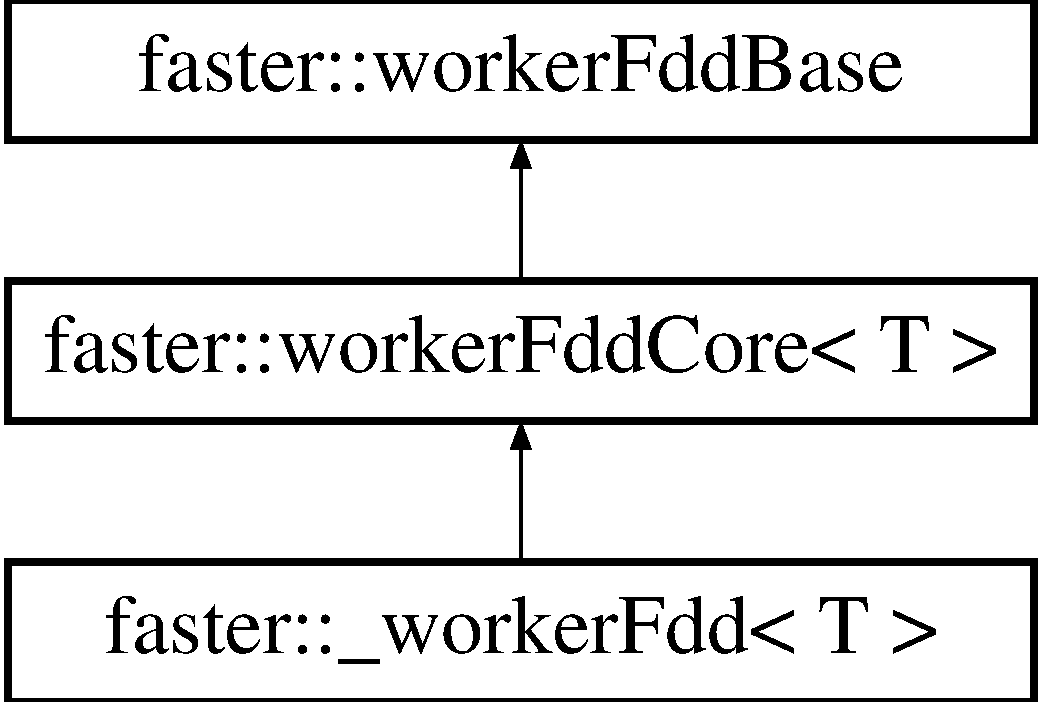
\includegraphics[height=3.000000cm]{classfaster_1_1__workerFdd}
\end{center}
\end{figure}
\subsection*{Public Member Functions}
\begin{DoxyCompactItemize}
\item 
\hypertarget{classfaster_1_1__workerFdd_a9f105bf8697f4f5332ccfb0fa7df8237}{}\label{classfaster_1_1__workerFdd_a9f105bf8697f4f5332ccfb0fa7df8237} 
{\bfseries \+\_\+worker\+Fdd} (unsigned int ident, \hyperlink{namespacefaster_aa8898687bc64536b60a3d5f365060cd6}{fdd\+Type} t)
\item 
\hypertarget{classfaster_1_1__workerFdd_ac8d6d1240857a56c57f5d85b6a4b67f5}{}\label{classfaster_1_1__workerFdd_ac8d6d1240857a56c57f5d85b6a4b67f5} 
{\bfseries \+\_\+worker\+Fdd} (unsigned int ident, \hyperlink{namespacefaster_aa8898687bc64536b60a3d5f365060cd6}{fdd\+Type} t, size\+\_\+t size)
\item 
\hypertarget{classfaster_1_1__workerFdd_a7031d0b585393f6e5a6ecc5e675a98ff}{}\label{classfaster_1_1__workerFdd_a7031d0b585393f6e5a6ecc5e675a98ff} 
void {\bfseries set\+Data} (T $\ast$data, size\+\_\+t size)
\item 
\hypertarget{classfaster_1_1__workerFdd_a18e7f4165cbd37d37f5759040b107cce}{}\label{classfaster_1_1__workerFdd_a18e7f4165cbd37d37f5759040b107cce} 
void {\bfseries set\+Data} (void $\ast$d U\+N\+U\+S\+ED, size\+\_\+t size U\+N\+U\+S\+ED)
\item 
\hypertarget{classfaster_1_1__workerFdd_ae2a8d9f60a3a0591f23dd5918451cecf}{}\label{classfaster_1_1__workerFdd_ae2a8d9f60a3a0591f23dd5918451cecf} 
void {\bfseries set\+Data} (void $\ast$d U\+N\+U\+S\+ED, size\+\_\+t $\ast$line\+Sizes U\+N\+U\+S\+ED, size\+\_\+t size U\+N\+U\+S\+ED)
\item 
\hypertarget{classfaster_1_1__workerFdd_a26f3dbf1187402ecd029a3ff1bf5f849}{}\label{classfaster_1_1__workerFdd_a26f3dbf1187402ecd029a3ff1bf5f849} 
void {\bfseries set\+Data} (void $\ast$k U\+N\+U\+S\+ED, void $\ast$d U\+N\+U\+S\+ED, size\+\_\+t $\ast$line\+Sizes U\+N\+U\+S\+ED, size\+\_\+t size U\+N\+U\+S\+ED)
\item 
\hypertarget{classfaster_1_1__workerFdd_a2439827c0e48411f92437a088f55b30f}{}\label{classfaster_1_1__workerFdd_a2439827c0e48411f92437a088f55b30f} 
void {\bfseries set\+Data\+Raw} (void $\ast$data, size\+\_\+t size) override
\item 
\hypertarget{classfaster_1_1__workerFdd_a236aaba89ce634bce445cfc8e00b0af1}{}\label{classfaster_1_1__workerFdd_a236aaba89ce634bce445cfc8e00b0af1} 
void {\bfseries set\+Data\+Raw} (void $\ast$data U\+N\+U\+S\+ED, size\+\_\+t $\ast$list\+Sizes U\+N\+U\+S\+ED, size\+\_\+t size U\+N\+U\+S\+ED) override
\item 
\hypertarget{classfaster_1_1__workerFdd_ad8d2388bc738798cb842f05abe3a232f}{}\label{classfaster_1_1__workerFdd_ad8d2388bc738798cb842f05abe3a232f} 
size\+\_\+t $\ast$ {\bfseries get\+Line\+Sizes} ()
\item 
\hypertarget{classfaster_1_1__workerFdd_a34cd7025c01c615d8da5b2994c3cd4fb}{}\label{classfaster_1_1__workerFdd_a34cd7025c01c615d8da5b2994c3cd4fb} 
void {\bfseries insert} (void $\ast$k, void $\ast$in, size\+\_\+t s)
\item 
\hypertarget{classfaster_1_1__workerFdd_a7c870a264f47310d61d4dc388d7fb588}{}\label{classfaster_1_1__workerFdd_a7c870a264f47310d61d4dc388d7fb588} 
void {\bfseries insertl} (void $\ast$in)
\item 
\hypertarget{classfaster_1_1__workerFdd_a16d0b3a72dee9067c78e6de5c00344d5}{}\label{classfaster_1_1__workerFdd_a16d0b3a72dee9067c78e6de5c00344d5} 
void {\bfseries insert} (T \&in)
\item 
\hypertarget{classfaster_1_1__workerFdd_aa4e0cbecfd3b70916364afb85ebbb042}{}\label{classfaster_1_1__workerFdd_aa4e0cbecfd3b70916364afb85ebbb042} 
void {\bfseries insert} (T $\ast$in U\+N\+U\+S\+ED, size\+\_\+t s U\+N\+U\+S\+ED)
\item 
\hypertarget{classfaster_1_1__workerFdd_af8d23cf110e95bd4a57ed8911e462fcd}{}\label{classfaster_1_1__workerFdd_af8d23cf110e95bd4a57ed8911e462fcd} 
void {\bfseries insert} (std\+::deque$<$ T $>$ \&in)
\item 
\hypertarget{classfaster_1_1__workerFdd_a5294bdf9244698046005cd985fc32047}{}\label{classfaster_1_1__workerFdd_a5294bdf9244698046005cd985fc32047} 
void {\bfseries insert} (std\+::deque$<$ std\+::pair$<$ T $\ast$, size\+\_\+t $>$$>$ \&in U\+N\+U\+S\+ED)
\item 
\hypertarget{classfaster_1_1__workerFdd_a77120c8d7ec05e6683acc699dfa86743}{}\label{classfaster_1_1__workerFdd_a77120c8d7ec05e6683acc699dfa86743} 
void {\bfseries apply} (void $\ast$func, \hyperlink{namespacefaster_a64379512d12d41c6e58f176939abfd80}{fdd\+Op\+Type} op, \hyperlink{classfaster_1_1workerFddBase}{worker\+Fdd\+Base} $\ast$dest, \hyperlink{classfaster_1_1fastCommBuffer}{fast\+Comm\+Buffer} \&buffer)
\item 
\hypertarget{classfaster_1_1__workerFdd_a5571e749cf6d7c1ce83e1a2d242d0240}{}\label{classfaster_1_1__workerFdd_a5571e749cf6d7c1ce83e1a2d242d0240} 
void {\bfseries collect} (\hyperlink{classfaster_1_1fastComm}{fast\+Comm} $\ast$comm) override
\item 
\hypertarget{classfaster_1_1__workerFdd_af988c35b5529ae5536e8acdcc9175a4d}{}\label{classfaster_1_1__workerFdd_af988c35b5529ae5536e8acdcc9175a4d} 
{\footnotesize template$<$typename U $>$ }\\void {\bfseries map} (\hyperlink{classfaster_1_1workerFddBase}{worker\+Fdd\+Base} $\ast$dest, map\+P\+FunctionP$<$ T, U $>$ map\+Func)
\item 
\hypertarget{classfaster_1_1__workerFdd_aec9174d171f08ebdb473b9c2f8c15a37}{}\label{classfaster_1_1__workerFdd_aec9174d171f08ebdb473b9c2f8c15a37} 
{\footnotesize template$<$typename U $>$ }\\void {\bfseries map} (\hyperlink{classfaster_1_1workerFddBase}{worker\+Fdd\+Base} $\ast$dest, Pmap\+P\+FunctionP$<$ T, U $>$ map\+Func)
\item 
\hypertarget{classfaster_1_1__workerFdd_a769b5239b6a8bfa0ec50e5bbd4577ef1}{}\label{classfaster_1_1__workerFdd_a769b5239b6a8bfa0ec50e5bbd4577ef1} 
{\footnotesize template$<$typename L , typename U $>$ }\\void {\bfseries map} (\hyperlink{classfaster_1_1workerFddBase}{worker\+Fdd\+Base} $\ast$dest, Imap\+P\+FunctionP$<$ T, L, U $>$ map\+Func)
\item 
\hypertarget{classfaster_1_1__workerFdd_ab448efbf81740e064306dd0a598a82f9}{}\label{classfaster_1_1__workerFdd_ab448efbf81740e064306dd0a598a82f9} 
{\footnotesize template$<$typename L , typename U $>$ }\\void {\bfseries map} (\hyperlink{classfaster_1_1workerFddBase}{worker\+Fdd\+Base} $\ast$dest, I\+Pmap\+P\+FunctionP$<$ T, L, U $>$ map\+Func)
\item 
\hypertarget{classfaster_1_1__workerFdd_a112f39ff204793ed31d9db8f08669bfd}{}\label{classfaster_1_1__workerFdd_a112f39ff204793ed31d9db8f08669bfd} 
{\footnotesize template$<$typename U $>$ }\\void {\bfseries bulk\+Map} (\hyperlink{classfaster_1_1workerFddBase}{worker\+Fdd\+Base} $\ast$dest, bulk\+Map\+P\+FunctionP$<$ T, U $>$ bulk\+Map\+Func)
\item 
\hypertarget{classfaster_1_1__workerFdd_adcbf8236e45778164fa89a99f471af97}{}\label{classfaster_1_1__workerFdd_adcbf8236e45778164fa89a99f471af97} 
{\footnotesize template$<$typename U $>$ }\\void {\bfseries bulk\+Map} (\hyperlink{classfaster_1_1workerFddBase}{worker\+Fdd\+Base} $\ast$dest, Pbulk\+Map\+P\+FunctionP$<$ T, U $>$ bulk\+Map\+Func)
\item 
\hypertarget{classfaster_1_1__workerFdd_aa97df61674d94be20272c3dcb02eb297}{}\label{classfaster_1_1__workerFdd_aa97df61674d94be20272c3dcb02eb297} 
{\footnotesize template$<$typename L , typename U $>$ }\\void {\bfseries bulk\+Map} (\hyperlink{classfaster_1_1workerFddBase}{worker\+Fdd\+Base} $\ast$dest, Ibulk\+Map\+P\+FunctionP$<$ T, L, U $>$ bulk\+Map\+Func)
\item 
\hypertarget{classfaster_1_1__workerFdd_a52ae456a7934f59f2ae1e174411eeda2}{}\label{classfaster_1_1__workerFdd_a52ae456a7934f59f2ae1e174411eeda2} 
{\footnotesize template$<$typename L , typename U $>$ }\\void {\bfseries bulk\+Map} (\hyperlink{classfaster_1_1workerFddBase}{worker\+Fdd\+Base} $\ast$dest, I\+Pbulk\+Map\+P\+FunctionP$<$ T, L, U $>$ bulk\+Map\+Func)
\item 
\hypertarget{classfaster_1_1__workerFdd_a82e09ab6af244695821c5ac58069baf3}{}\label{classfaster_1_1__workerFdd_a82e09ab6af244695821c5ac58069baf3} 
{\footnotesize template$<$typename U $>$ }\\void {\bfseries flat\+Map} (\hyperlink{classfaster_1_1workerFddBase}{worker\+Fdd\+Base} $\ast$dest, flat\+Map\+P\+FunctionP$<$ T, U $>$ flat\+Map\+Func)
\item 
\hypertarget{classfaster_1_1__workerFdd_a6730755a899115bbb8ffb39c349148de}{}\label{classfaster_1_1__workerFdd_a6730755a899115bbb8ffb39c349148de} 
{\footnotesize template$<$typename U $>$ }\\void {\bfseries flat\+Map} (\hyperlink{classfaster_1_1workerFddBase}{worker\+Fdd\+Base} $\ast$dest, Pflat\+Map\+P\+FunctionP$<$ T, U $>$ flat\+Map\+Func)
\item 
\hypertarget{classfaster_1_1__workerFdd_ac3949737c498f3405e710b6ba27f637d}{}\label{classfaster_1_1__workerFdd_ac3949737c498f3405e710b6ba27f637d} 
{\footnotesize template$<$typename L , typename U $>$ }\\void {\bfseries flat\+Map} (\hyperlink{classfaster_1_1workerFddBase}{worker\+Fdd\+Base} $\ast$dest, Iflat\+Map\+P\+FunctionP$<$ T, L, U $>$ flat\+Map\+Func)
\item 
\hypertarget{classfaster_1_1__workerFdd_a432dc7be45d8e85eeed57df0e62b7016}{}\label{classfaster_1_1__workerFdd_a432dc7be45d8e85eeed57df0e62b7016} 
{\footnotesize template$<$typename L , typename U $>$ }\\void {\bfseries flat\+Map} (\hyperlink{classfaster_1_1workerFddBase}{worker\+Fdd\+Base} $\ast$dest, I\+Pflat\+Map\+P\+FunctionP$<$ T, L, U $>$ flat\+Map\+Func)
\item 
\hypertarget{classfaster_1_1__workerFdd_a986e1a834767a0e7484ff6ef938d00fe}{}\label{classfaster_1_1__workerFdd_a986e1a834767a0e7484ff6ef938d00fe} 
{\footnotesize template$<$typename U $>$ }\\void {\bfseries bulk\+Flat\+Map} (\hyperlink{classfaster_1_1workerFddBase}{worker\+Fdd\+Base} $\ast$dest, bulk\+Flat\+Map\+P\+FunctionP$<$ T, U $>$ bulk\+Flat\+Map\+Func)
\item 
\hypertarget{classfaster_1_1__workerFdd_a373a14d5b681adee6bd1cbd3d596a881}{}\label{classfaster_1_1__workerFdd_a373a14d5b681adee6bd1cbd3d596a881} 
{\footnotesize template$<$typename U $>$ }\\void {\bfseries bulk\+Flat\+Map} (\hyperlink{classfaster_1_1workerFddBase}{worker\+Fdd\+Base} $\ast$dest, Pbulk\+Flat\+Map\+P\+FunctionP$<$ T, U $>$ bulk\+Flat\+Map\+Func)
\item 
\hypertarget{classfaster_1_1__workerFdd_a95e2522e743e7f1c3c9977355739b19b}{}\label{classfaster_1_1__workerFdd_a95e2522e743e7f1c3c9977355739b19b} 
{\footnotesize template$<$typename L , typename U $>$ }\\void {\bfseries bulk\+Flat\+Map} (\hyperlink{classfaster_1_1workerFddBase}{worker\+Fdd\+Base} $\ast$dest, Ibulk\+Flat\+Map\+P\+FunctionP$<$ T, L, U $>$ bulk\+Flat\+Map\+Func)
\item 
\hypertarget{classfaster_1_1__workerFdd_aae7a3c9c93468112b071b2441a34b725}{}\label{classfaster_1_1__workerFdd_aae7a3c9c93468112b071b2441a34b725} 
{\footnotesize template$<$typename L , typename U $>$ }\\void {\bfseries bulk\+Flat\+Map} (\hyperlink{classfaster_1_1workerFddBase}{worker\+Fdd\+Base} $\ast$dest, I\+Pbulk\+Flat\+Map\+P\+FunctionP$<$ T, L, U $>$ bulk\+Flat\+Map\+Func)
\end{DoxyCompactItemize}
\subsection*{Additional Inherited Members}


The documentation for this class was generated from the following files\+:\begin{DoxyCompactItemize}
\item 
/home/mtcs/pesquisa/faster/faster.\+git/src/include/\+\_\+worker\+Fdd.\+h\item 
/home/mtcs/pesquisa/faster/faster.\+git/src/libfaster/\+\_\+worker\+Fdd.\+cpp\item 
/home/mtcs/pesquisa/faster/faster.\+git/src/libfaster/worker\+P\+Fdd.\+cpp\end{DoxyCompactItemize}

\hypertarget{classfaster_1_1__workerFdd_3_01T_01_5_01_4}{}\section{faster\+:\+:\+\_\+worker\+Fdd$<$ T $\ast$ $>$ Class Template Reference}
\label{classfaster_1_1__workerFdd_3_01T_01_5_01_4}\index{faster\+::\+\_\+worker\+Fdd$<$ T $\ast$ $>$@{faster\+::\+\_\+worker\+Fdd$<$ T $\ast$ $>$}}
Inheritance diagram for faster\+:\+:\+\_\+worker\+Fdd$<$ T $\ast$ $>$\+:\begin{figure}[H]
\begin{center}
\leavevmode
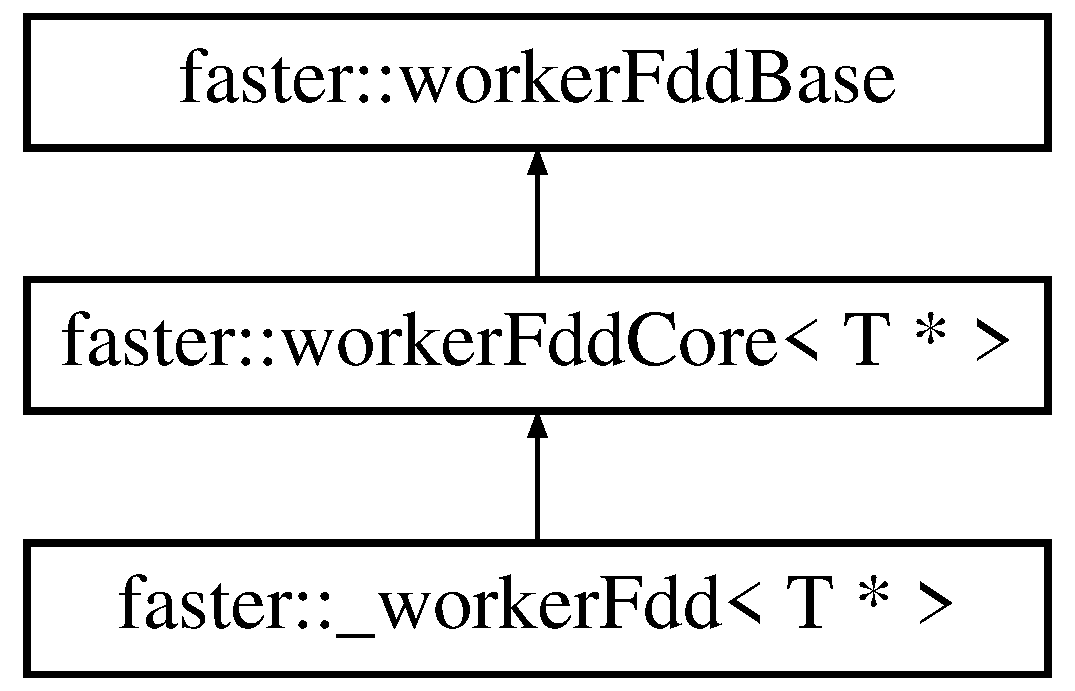
\includegraphics[height=3.000000cm]{classfaster_1_1__workerFdd_3_01T_01_5_01_4}
\end{center}
\end{figure}


\subsection{Description}
\subsubsection*{template$<$class T$>$\newline
class faster\+::\+\_\+worker\+Fdd$<$ T $\ast$ $>$}



Definition at line 186 of file \+\_\+worker\+Fdd.\+h.

\subsection*{Public Member Functions}
\begin{DoxyCompactItemize}
\item 
\hypertarget{classfaster_1_1__workerFdd_3_01T_01_5_01_4_a47e31872160658985595a45cb4a546a7}{}\label{classfaster_1_1__workerFdd_3_01T_01_5_01_4_a47e31872160658985595a45cb4a546a7} 
{\bfseries \+\_\+worker\+Fdd} (unsigned int ident, \hyperlink{namespacefaster_aa8898687bc64536b60a3d5f365060cd6}{fdd\+Type} t)
\item 
\hypertarget{classfaster_1_1__workerFdd_3_01T_01_5_01_4_a9bdf0205db584c51f2160d158629b979}{}\label{classfaster_1_1__workerFdd_3_01T_01_5_01_4_a9bdf0205db584c51f2160d158629b979} 
{\bfseries \+\_\+worker\+Fdd} (unsigned int ident, \hyperlink{namespacefaster_aa8898687bc64536b60a3d5f365060cd6}{fdd\+Type} t, size\+\_\+t size)
\item 
\hypertarget{classfaster_1_1__workerFdd_3_01T_01_5_01_4_a6c828c7980659ae657bae25e4bbbf7b0}{}\label{classfaster_1_1__workerFdd_3_01T_01_5_01_4_a6c828c7980659ae657bae25e4bbbf7b0} 
void {\bfseries set\+Data} (T $\ast$$\ast$data, size\+\_\+t $\ast$line\+Sizes, size\+\_\+t size)
\item 
\hypertarget{classfaster_1_1__workerFdd_3_01T_01_5_01_4_ad6c9ec2e14d529ef574ed3031749baf1}{}\label{classfaster_1_1__workerFdd_3_01T_01_5_01_4_ad6c9ec2e14d529ef574ed3031749baf1} 
void {\bfseries set\+Data} (void $\ast$d U\+N\+U\+S\+ED, size\+\_\+t size U\+N\+U\+S\+ED)
\item 
\hypertarget{classfaster_1_1__workerFdd_3_01T_01_5_01_4_ab0b7a6bb56047036f6bf2a30f509303f}{}\label{classfaster_1_1__workerFdd_3_01T_01_5_01_4_ab0b7a6bb56047036f6bf2a30f509303f} 
void {\bfseries set\+Data} (void $\ast$data U\+N\+U\+S\+ED, size\+\_\+t $\ast$line\+Sizes U\+N\+U\+S\+ED, size\+\_\+t size U\+N\+U\+S\+ED)
\item 
\hypertarget{classfaster_1_1__workerFdd_3_01T_01_5_01_4_a697ae8111ed8aaad17c1d739894e449f}{}\label{classfaster_1_1__workerFdd_3_01T_01_5_01_4_a697ae8111ed8aaad17c1d739894e449f} 
void {\bfseries set\+Data} (void $\ast$k U\+N\+U\+S\+ED, void $\ast$d U\+N\+U\+S\+ED, size\+\_\+t $\ast$line\+Sizes U\+N\+U\+S\+ED, size\+\_\+t size U\+N\+U\+S\+ED)
\item 
\hypertarget{classfaster_1_1__workerFdd_3_01T_01_5_01_4_a4718bba9d9bf44a30c74bd38b426a9cd}{}\label{classfaster_1_1__workerFdd_3_01T_01_5_01_4_a4718bba9d9bf44a30c74bd38b426a9cd} 
void {\bfseries set\+Data\+Raw} (void $\ast$data U\+N\+U\+S\+ED, size\+\_\+t size U\+N\+U\+S\+ED) override
\item 
\hypertarget{classfaster_1_1__workerFdd_3_01T_01_5_01_4_a4246404cbe09e51acf1f78af85e2ef13}{}\label{classfaster_1_1__workerFdd_3_01T_01_5_01_4_a4246404cbe09e51acf1f78af85e2ef13} 
void {\bfseries set\+Data\+Raw} (void $\ast$data, size\+\_\+t $\ast$line\+Sizes, size\+\_\+t size) override
\item 
\hypertarget{classfaster_1_1__workerFdd_3_01T_01_5_01_4_a18ba8f65a2811cb956b547ecb2982417}{}\label{classfaster_1_1__workerFdd_3_01T_01_5_01_4_a18ba8f65a2811cb956b547ecb2982417} 
size\+\_\+t $\ast$ {\bfseries get\+Line\+Sizes} ()
\item 
\hypertarget{classfaster_1_1__workerFdd_3_01T_01_5_01_4_ad0b49f344ef0a582f1cf01973832b570}{}\label{classfaster_1_1__workerFdd_3_01T_01_5_01_4_ad0b49f344ef0a582f1cf01973832b570} 
void {\bfseries insert} (void $\ast$k, void $\ast$in, size\+\_\+t s)
\item 
\hypertarget{classfaster_1_1__workerFdd_3_01T_01_5_01_4_aaa99e6a10c37391910d4aba2342ee618}{}\label{classfaster_1_1__workerFdd_3_01T_01_5_01_4_aaa99e6a10c37391910d4aba2342ee618} 
void {\bfseries insertl} (void $\ast$in)
\item 
\hypertarget{classfaster_1_1__workerFdd_3_01T_01_5_01_4_a43bf6522a9d2017c184e64f8be51698b}{}\label{classfaster_1_1__workerFdd_3_01T_01_5_01_4_a43bf6522a9d2017c184e64f8be51698b} 
void {\bfseries insert} (T \&in)
\item 
\hypertarget{classfaster_1_1__workerFdd_3_01T_01_5_01_4_ad3dabe7a5a99426a605e567cec8fe9d9}{}\label{classfaster_1_1__workerFdd_3_01T_01_5_01_4_ad3dabe7a5a99426a605e567cec8fe9d9} 
void {\bfseries insert} (T $\ast$\&in, size\+\_\+t s)
\item 
\hypertarget{classfaster_1_1__workerFdd_3_01T_01_5_01_4_a29976297df6221272c98ed2b83545775}{}\label{classfaster_1_1__workerFdd_3_01T_01_5_01_4_a29976297df6221272c98ed2b83545775} 
void {\bfseries insert} (std\+::deque$<$ T $>$ \&in)
\item 
\hypertarget{classfaster_1_1__workerFdd_3_01T_01_5_01_4_aa3fde5f3b38bb5e905f8d668526a0ede}{}\label{classfaster_1_1__workerFdd_3_01T_01_5_01_4_aa3fde5f3b38bb5e905f8d668526a0ede} 
void {\bfseries insert} (std\+::deque$<$ std\+::pair$<$ T $\ast$, size\+\_\+t $>$ $>$ \&in)
\item 
\hypertarget{classfaster_1_1__workerFdd_3_01T_01_5_01_4_a249018ae1fe5990f9b081c8519fccf13}{}\label{classfaster_1_1__workerFdd_3_01T_01_5_01_4_a249018ae1fe5990f9b081c8519fccf13} 
void {\bfseries apply} (void $\ast$func, \hyperlink{namespacefaster_a64379512d12d41c6e58f176939abfd80}{fdd\+Op\+Type} op, \hyperlink{classfaster_1_1workerFddBase}{worker\+Fdd\+Base} $\ast$dest, \hyperlink{classfaster_1_1fastCommBuffer}{fast\+Comm\+Buffer} \&buffer)
\item 
\hypertarget{classfaster_1_1__workerFdd_3_01T_01_5_01_4_a3548e79c7a505468d842a6bb49e392f3}{}\label{classfaster_1_1__workerFdd_3_01T_01_5_01_4_a3548e79c7a505468d842a6bb49e392f3} 
void {\bfseries collect} (\hyperlink{classfaster_1_1fastComm}{fast\+Comm} $\ast$comm) override
\end{DoxyCompactItemize}
\subsection*{Additional Inherited Members}


The documentation for this class was generated from the following file\+:\begin{DoxyCompactItemize}
\item 
/home/mtcs/pesquisa/faster/faster.\+git/src/include/\+\_\+worker\+Fdd.\+h\end{DoxyCompactItemize}

\hypertarget{classfaster_1_1__workerIFdd}{}\section{faster\+:\+:\+\_\+worker\+I\+Fdd$<$ K, T $>$ Class Template Reference}
\label{classfaster_1_1__workerIFdd}\index{faster\+::\+\_\+worker\+I\+Fdd$<$ K, T $>$@{faster\+::\+\_\+worker\+I\+Fdd$<$ K, T $>$}}
Inheritance diagram for faster\+:\+:\+\_\+worker\+I\+Fdd$<$ K, T $>$\+:\begin{figure}[H]
\begin{center}
\leavevmode
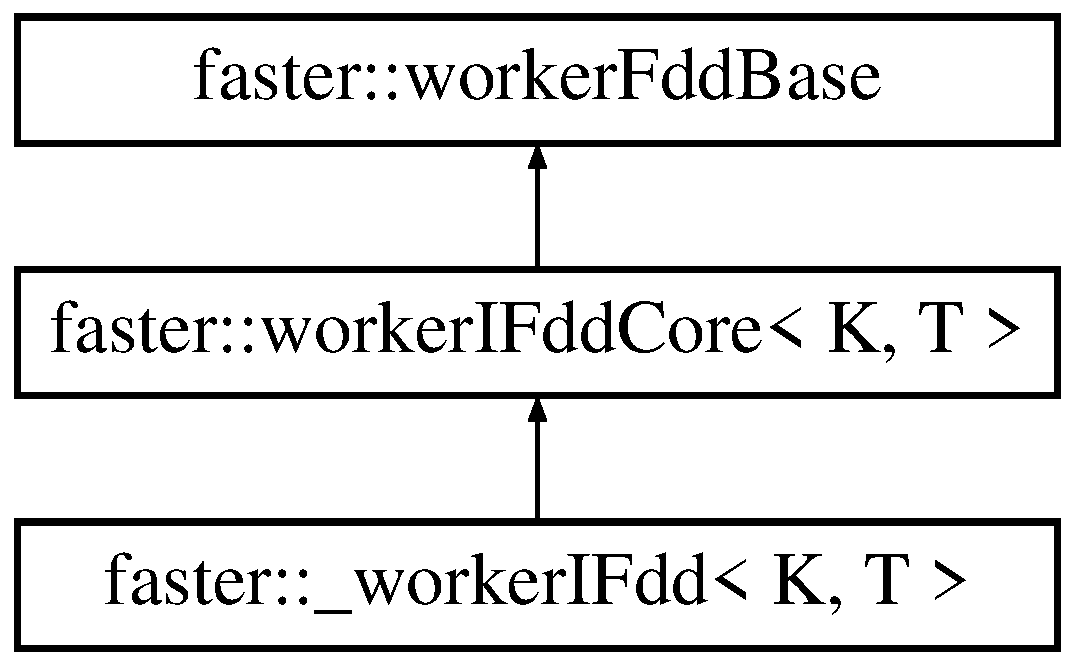
\includegraphics[height=3.000000cm]{classfaster_1_1__workerIFdd}
\end{center}
\end{figure}
\subsection*{Public Member Functions}
\begin{DoxyCompactItemize}
\item 
\hypertarget{classfaster_1_1__workerIFdd_a08037ef118ef3e86a3b1926f4d11d443}{}\label{classfaster_1_1__workerIFdd_a08037ef118ef3e86a3b1926f4d11d443} 
{\bfseries \+\_\+worker\+I\+Fdd} (unsigned int ident, \hyperlink{namespacefaster_aa8898687bc64536b60a3d5f365060cd6}{fdd\+Type} kt, \hyperlink{namespacefaster_aa8898687bc64536b60a3d5f365060cd6}{fdd\+Type} t)
\item 
\hypertarget{classfaster_1_1__workerIFdd_a310dd5f9799da46d3fecf15c917a5b46}{}\label{classfaster_1_1__workerIFdd_a310dd5f9799da46d3fecf15c917a5b46} 
{\bfseries \+\_\+worker\+I\+Fdd} (unsigned int ident, \hyperlink{namespacefaster_aa8898687bc64536b60a3d5f365060cd6}{fdd\+Type} kt, \hyperlink{namespacefaster_aa8898687bc64536b60a3d5f365060cd6}{fdd\+Type} t, size\+\_\+t size)
\item 
\hypertarget{classfaster_1_1__workerIFdd_a7c25eaec0cb983ca8d3891886f4d2e3e}{}\label{classfaster_1_1__workerIFdd_a7c25eaec0cb983ca8d3891886f4d2e3e} 
void {\bfseries set\+Data} (K $\ast$keys, T $\ast$data, size\+\_\+t size)
\item 
\hypertarget{classfaster_1_1__workerIFdd_a72512bdb22ef328a7eaa98af26c637c9}{}\label{classfaster_1_1__workerIFdd_a72512bdb22ef328a7eaa98af26c637c9} 
void {\bfseries set\+Data} (void $\ast$keys, void $\ast$data, size\+\_\+t size)
\item 
\hypertarget{classfaster_1_1__workerIFdd_a612ec6f32a16bb384b353f06063573c0}{}\label{classfaster_1_1__workerIFdd_a612ec6f32a16bb384b353f06063573c0} 
void {\bfseries set\+Data} (void $\ast$keys, void $\ast$data, size\+\_\+t $\ast$line\+Sizes U\+N\+U\+S\+ED, size\+\_\+t size)
\item 
\hypertarget{classfaster_1_1__workerIFdd_afe2037df84a871a1d1971295460de648}{}\label{classfaster_1_1__workerIFdd_afe2037df84a871a1d1971295460de648} 
void {\bfseries set\+Data\+Raw} (void $\ast$keys, void $\ast$data, size\+\_\+t size) override
\item 
\hypertarget{classfaster_1_1__workerIFdd_ae8acb90658c5051a34a71bc03e43bf1e}{}\label{classfaster_1_1__workerIFdd_ae8acb90658c5051a34a71bc03e43bf1e} 
void {\bfseries set\+Data\+Raw} (void $\ast$keys U\+N\+U\+S\+ED, void $\ast$data U\+N\+U\+S\+ED, size\+\_\+t $\ast$line\+Sizes U\+N\+U\+S\+ED, size\+\_\+t size U\+N\+U\+S\+ED) override
\item 
\hypertarget{classfaster_1_1__workerIFdd_a9c0862beb4226e84a7b8f82f8841feac}{}\label{classfaster_1_1__workerIFdd_a9c0862beb4226e84a7b8f82f8841feac} 
size\+\_\+t $\ast$ {\bfseries get\+Line\+Sizes} ()
\item 
\hypertarget{classfaster_1_1__workerIFdd_aa806f1fef09dbeaaca74b09821e60935}{}\label{classfaster_1_1__workerIFdd_aa806f1fef09dbeaaca74b09821e60935} 
void {\bfseries insert} (void $\ast$k, void $\ast$in, size\+\_\+t s)
\item 
\hypertarget{classfaster_1_1__workerIFdd_a0c1716a3b4fb62fa1c4c9ffe95761ef4}{}\label{classfaster_1_1__workerIFdd_a0c1716a3b4fb62fa1c4c9ffe95761ef4} 
void {\bfseries insertl} (void $\ast$in)
\item 
\hypertarget{classfaster_1_1__workerIFdd_ac248aade1f81e85a4f8a48ba8b6fb9b7}{}\label{classfaster_1_1__workerIFdd_ac248aade1f81e85a4f8a48ba8b6fb9b7} 
void {\bfseries insert} (K \&key, T \&in)
\item 
\hypertarget{classfaster_1_1__workerIFdd_a02d3affac82eaf9e1fe524e5cbcd44d1}{}\label{classfaster_1_1__workerIFdd_a02d3affac82eaf9e1fe524e5cbcd44d1} 
void {\bfseries insert} (std\+::deque$<$ std\+::pair$<$ K, T $>$ $>$ \&in)
\item 
\hypertarget{classfaster_1_1__workerIFdd_aa9bd2045e6a85cd39f868ad50fbcb5c4}{}\label{classfaster_1_1__workerIFdd_aa9bd2045e6a85cd39f868ad50fbcb5c4} 
void {\bfseries apply} (void $\ast$func, \hyperlink{namespacefaster_a64379512d12d41c6e58f176939abfd80}{fdd\+Op\+Type} op, \hyperlink{classfaster_1_1workerFddBase}{worker\+Fdd\+Base} $\ast$dest, \hyperlink{classfaster_1_1fastCommBuffer}{fast\+Comm\+Buffer} \&buffer)
\item 
\hypertarget{classfaster_1_1__workerIFdd_a256bac01a1de34d3debeca359783f9f6}{}\label{classfaster_1_1__workerIFdd_a256bac01a1de34d3debeca359783f9f6} 
void {\bfseries collect} (\hyperlink{classfaster_1_1fastComm}{fast\+Comm} $\ast$comm) override
\item 
\hypertarget{classfaster_1_1__workerIFdd_a4038e3b76165af8c5b7e867336ec1bce}{}\label{classfaster_1_1__workerIFdd_a4038e3b76165af8c5b7e867336ec1bce} 
{\footnotesize template$<$typename L , typename U $>$ }\\void {\bfseries map} (\hyperlink{classfaster_1_1workerFddBase}{worker\+Fdd\+Base} $\ast$dest, Imap\+I\+P\+FunctionP$<$ K, T, L, U $>$ map\+Func)
\item 
\hypertarget{classfaster_1_1__workerIFdd_a183e0438a65c27ba0b5182679f87afb9}{}\label{classfaster_1_1__workerIFdd_a183e0438a65c27ba0b5182679f87afb9} 
{\footnotesize template$<$typename L , typename U $>$ }\\void {\bfseries map} (\hyperlink{classfaster_1_1workerFddBase}{worker\+Fdd\+Base} $\ast$dest, I\+Pmap\+I\+P\+FunctionP$<$ K, T, L, U $>$ map\+Func)
\item 
\hypertarget{classfaster_1_1__workerIFdd_a1370b613f6bcd5113be986d45a5a7f6a}{}\label{classfaster_1_1__workerIFdd_a1370b613f6bcd5113be986d45a5a7f6a} 
{\footnotesize template$<$typename U $>$ }\\void {\bfseries map} (\hyperlink{classfaster_1_1workerFddBase}{worker\+Fdd\+Base} $\ast$dest, map\+I\+P\+FunctionP$<$ K, T, U $>$ map\+Func)
\item 
\hypertarget{classfaster_1_1__workerIFdd_aacd4131321c22e4cb621a0378590c218}{}\label{classfaster_1_1__workerIFdd_aacd4131321c22e4cb621a0378590c218} 
{\footnotesize template$<$typename U $>$ }\\void {\bfseries map} (\hyperlink{classfaster_1_1workerFddBase}{worker\+Fdd\+Base} $\ast$dest, Pmap\+I\+P\+FunctionP$<$ K, T, U $>$ map\+Func)
\item 
\hypertarget{classfaster_1_1__workerIFdd_af615ca291ae54700159a46bafb170217}{}\label{classfaster_1_1__workerIFdd_af615ca291ae54700159a46bafb170217} 
{\footnotesize template$<$typename L , typename U $>$ }\\void {\bfseries bulk\+Map} (\hyperlink{classfaster_1_1workerFddBase}{worker\+Fdd\+Base} $\ast$dest, Ibulk\+Map\+I\+P\+FunctionP$<$ K, T, L, U $>$ bulk\+Map\+Func)
\item 
\hypertarget{classfaster_1_1__workerIFdd_ad273de2e3d16220c260d57a56ac66b8c}{}\label{classfaster_1_1__workerIFdd_ad273de2e3d16220c260d57a56ac66b8c} 
{\footnotesize template$<$typename L , typename U $>$ }\\void {\bfseries bulk\+Map} (\hyperlink{classfaster_1_1workerFddBase}{worker\+Fdd\+Base} $\ast$dest, I\+Pbulk\+Map\+I\+P\+FunctionP$<$ K, T, L, U $>$ bulk\+Map\+Func)
\item 
\hypertarget{classfaster_1_1__workerIFdd_af5248951f3ceb15dbb64eeeb51d21582}{}\label{classfaster_1_1__workerIFdd_af5248951f3ceb15dbb64eeeb51d21582} 
{\footnotesize template$<$typename U $>$ }\\void {\bfseries bulk\+Map} (\hyperlink{classfaster_1_1workerFddBase}{worker\+Fdd\+Base} $\ast$dest, bulk\+Map\+I\+P\+FunctionP$<$ K, T, U $>$ bulk\+Map\+Func)
\item 
\hypertarget{classfaster_1_1__workerIFdd_ac9f95a47678e286a47dfb3b554d6d700}{}\label{classfaster_1_1__workerIFdd_ac9f95a47678e286a47dfb3b554d6d700} 
{\footnotesize template$<$typename U $>$ }\\void {\bfseries bulk\+Map} (\hyperlink{classfaster_1_1workerFddBase}{worker\+Fdd\+Base} $\ast$dest, Pbulk\+Map\+I\+P\+FunctionP$<$ K, T, U $>$ bulk\+Map\+Func)
\item 
\hypertarget{classfaster_1_1__workerIFdd_aa17b7485c48adda5f291fd05993401be}{}\label{classfaster_1_1__workerIFdd_aa17b7485c48adda5f291fd05993401be} 
{\footnotesize template$<$typename L , typename U $>$ }\\void {\bfseries flat\+Map} (\hyperlink{classfaster_1_1workerFddBase}{worker\+Fdd\+Base} $\ast$dest, Iflat\+Map\+I\+P\+FunctionP$<$ K, T, L, U $>$ flat\+Map\+Func)
\item 
\hypertarget{classfaster_1_1__workerIFdd_a01712706bef8983d5715d5008b8f3bc7}{}\label{classfaster_1_1__workerIFdd_a01712706bef8983d5715d5008b8f3bc7} 
{\footnotesize template$<$typename L , typename U $>$ }\\void {\bfseries flat\+Map} (\hyperlink{classfaster_1_1workerFddBase}{worker\+Fdd\+Base} $\ast$dest, I\+Pflat\+Map\+I\+P\+FunctionP$<$ K, T, L, U $>$ flat\+Map\+Func)
\item 
\hypertarget{classfaster_1_1__workerIFdd_addd948777947f39bb4676e3516b797fb}{}\label{classfaster_1_1__workerIFdd_addd948777947f39bb4676e3516b797fb} 
{\footnotesize template$<$typename U $>$ }\\void {\bfseries flat\+Map} (\hyperlink{classfaster_1_1workerFddBase}{worker\+Fdd\+Base} $\ast$dest, flat\+Map\+I\+P\+FunctionP$<$ K, T, U $>$ flat\+Map\+Func)
\item 
\hypertarget{classfaster_1_1__workerIFdd_ac3f559fafc3463630d8febb26f626796}{}\label{classfaster_1_1__workerIFdd_ac3f559fafc3463630d8febb26f626796} 
{\footnotesize template$<$typename U $>$ }\\void {\bfseries flat\+Map} (\hyperlink{classfaster_1_1workerFddBase}{worker\+Fdd\+Base} $\ast$dest, Pflat\+Map\+I\+P\+FunctionP$<$ K, T, U $>$ flat\+Map\+Func)
\item 
\hypertarget{classfaster_1_1__workerIFdd_a5953db5f9f01e5e6d746e79eeb70b44e}{}\label{classfaster_1_1__workerIFdd_a5953db5f9f01e5e6d746e79eeb70b44e} 
{\footnotesize template$<$typename L , typename U $>$ }\\void {\bfseries bulk\+Flat\+Map} (\hyperlink{classfaster_1_1workerFddBase}{worker\+Fdd\+Base} $\ast$dest, Ibulk\+Flat\+Map\+I\+P\+FunctionP$<$ K, T, L, U $>$ bulk\+Flat\+Map\+Func)
\item 
\hypertarget{classfaster_1_1__workerIFdd_af8a719a7aed1b3a7334add9f1068445e}{}\label{classfaster_1_1__workerIFdd_af8a719a7aed1b3a7334add9f1068445e} 
{\footnotesize template$<$typename L , typename U $>$ }\\void {\bfseries bulk\+Flat\+Map} (\hyperlink{classfaster_1_1workerFddBase}{worker\+Fdd\+Base} $\ast$dest, I\+Pbulk\+Flat\+Map\+I\+P\+FunctionP$<$ K, T, L, U $>$ bulk\+Flat\+Map\+Func)
\item 
\hypertarget{classfaster_1_1__workerIFdd_ab69516c39651ef1caa7200027fa70a32}{}\label{classfaster_1_1__workerIFdd_ab69516c39651ef1caa7200027fa70a32} 
{\footnotesize template$<$typename U $>$ }\\void {\bfseries bulk\+Flat\+Map} (\hyperlink{classfaster_1_1workerFddBase}{worker\+Fdd\+Base} $\ast$dest, bulk\+Flat\+Map\+I\+P\+FunctionP$<$ K, T, U $>$ bulk\+Flat\+Map\+Func)
\item 
\hypertarget{classfaster_1_1__workerIFdd_a7daca5d9561429cf47fc31b8d1256e7f}{}\label{classfaster_1_1__workerIFdd_a7daca5d9561429cf47fc31b8d1256e7f} 
{\footnotesize template$<$typename U $>$ }\\void {\bfseries bulk\+Flat\+Map} (\hyperlink{classfaster_1_1workerFddBase}{worker\+Fdd\+Base} $\ast$dest, Pbulk\+Flat\+Map\+I\+P\+FunctionP$<$ K, T, U $>$ bulk\+Flat\+Map\+Func)
\end{DoxyCompactItemize}
\subsection*{Additional Inherited Members}


The documentation for this class was generated from the following files\+:\begin{DoxyCompactItemize}
\item 
/home/mtcs/pesquisa/faster/faster.\+git/src/include/\+\_\+worker\+I\+Fdd.\+h\item 
/home/mtcs/pesquisa/faster/faster.\+git/src/libfaster/worker\+I\+Fdd.\+cpp\item 
/home/mtcs/pesquisa/faster/faster.\+git/src/libfaster/worker\+I\+Fdd\+Dependent.\+cpp\item 
/home/mtcs/pesquisa/faster/faster.\+git/src/libfaster/worker\+I\+P\+Fdd.\+cpp\item 
/home/mtcs/pesquisa/faster/faster.\+git/src/libfaster/worker\+I\+P\+Fdd\+Dependent.\+cpp\end{DoxyCompactItemize}

\hypertarget{classfaster_1_1__workerIFdd_3_01K_00_01T_01_5_01_4}{}\section{faster\+:\+:\+\_\+worker\+I\+Fdd$<$ K, T $\ast$ $>$ Class Template Reference}
\label{classfaster_1_1__workerIFdd_3_01K_00_01T_01_5_01_4}\index{faster\+::\+\_\+worker\+I\+Fdd$<$ K, T $\ast$ $>$@{faster\+::\+\_\+worker\+I\+Fdd$<$ K, T $\ast$ $>$}}
Inheritance diagram for faster\+:\+:\+\_\+worker\+I\+Fdd$<$ K, T $\ast$ $>$\+:\begin{figure}[H]
\begin{center}
\leavevmode
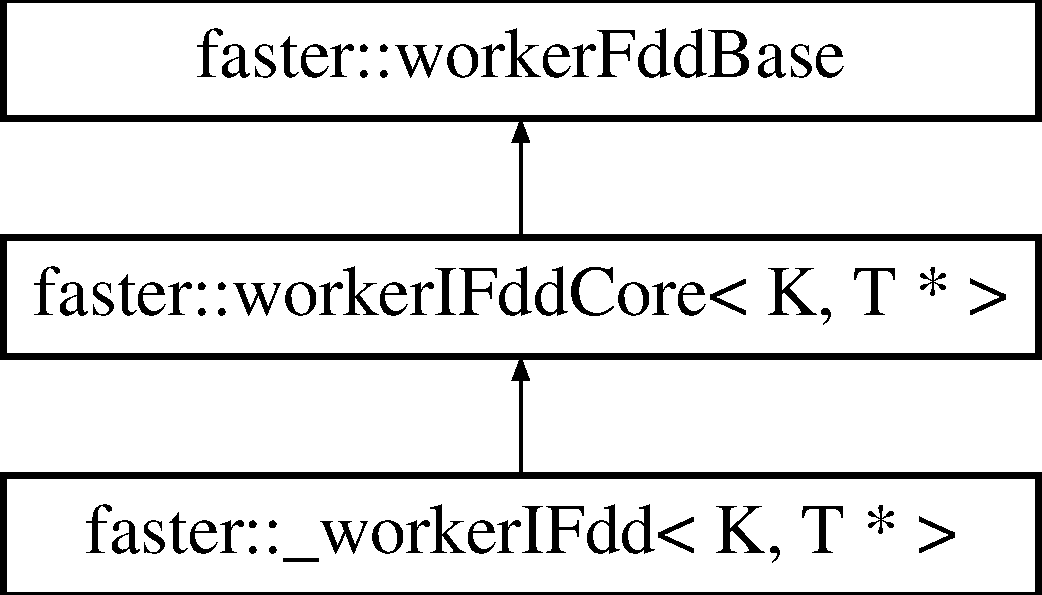
\includegraphics[height=3.000000cm]{classfaster_1_1__workerIFdd_3_01K_00_01T_01_5_01_4}
\end{center}
\end{figure}


\subsection{Description}
\subsubsection*{template$<$class K, class T$>$\newline
class faster\+::\+\_\+worker\+I\+Fdd$<$ K, T $\ast$ $>$}



Definition at line 258 of file \+\_\+worker\+I\+Fdd.\+h.

\subsection*{Public Member Functions}
\begin{DoxyCompactItemize}
\item 
\hypertarget{classfaster_1_1__workerIFdd_3_01K_00_01T_01_5_01_4_a9f0be9976988a83b3339d8387ff8e2e1}{}\label{classfaster_1_1__workerIFdd_3_01K_00_01T_01_5_01_4_a9f0be9976988a83b3339d8387ff8e2e1} 
{\bfseries \+\_\+worker\+I\+Fdd} (unsigned int ident, \hyperlink{namespacefaster_aa8898687bc64536b60a3d5f365060cd6}{fdd\+Type} kt, \hyperlink{namespacefaster_aa8898687bc64536b60a3d5f365060cd6}{fdd\+Type} t)
\item 
\hypertarget{classfaster_1_1__workerIFdd_3_01K_00_01T_01_5_01_4_a98d1388d2afd0339d5c04a985e6eb8d1}{}\label{classfaster_1_1__workerIFdd_3_01K_00_01T_01_5_01_4_a98d1388d2afd0339d5c04a985e6eb8d1} 
{\bfseries \+\_\+worker\+I\+Fdd} (unsigned int ident, \hyperlink{namespacefaster_aa8898687bc64536b60a3d5f365060cd6}{fdd\+Type} kt, \hyperlink{namespacefaster_aa8898687bc64536b60a3d5f365060cd6}{fdd\+Type} t, size\+\_\+t size)
\item 
\hypertarget{classfaster_1_1__workerIFdd_3_01K_00_01T_01_5_01_4_ab87f4b8c53a15b94190cbcbba67e8c8b}{}\label{classfaster_1_1__workerIFdd_3_01K_00_01T_01_5_01_4_ab87f4b8c53a15b94190cbcbba67e8c8b} 
void {\bfseries set\+Data} (K $\ast$keys, T $\ast$$\ast$data, size\+\_\+t $\ast$line\+Sizes, size\+\_\+t size)
\item 
\hypertarget{classfaster_1_1__workerIFdd_3_01K_00_01T_01_5_01_4_a08aa87e7f72eec843f350725d62b76ee}{}\label{classfaster_1_1__workerIFdd_3_01K_00_01T_01_5_01_4_a08aa87e7f72eec843f350725d62b76ee} 
void {\bfseries set\+Data} (void $\ast$keys U\+N\+U\+S\+ED, void $\ast$data U\+N\+U\+S\+ED, size\+\_\+t size U\+N\+U\+S\+ED)
\item 
\hypertarget{classfaster_1_1__workerIFdd_3_01K_00_01T_01_5_01_4_a2a73efd212717ed23a1e406635d80f5d}{}\label{classfaster_1_1__workerIFdd_3_01K_00_01T_01_5_01_4_a2a73efd212717ed23a1e406635d80f5d} 
void {\bfseries set\+Data} (void $\ast$keys, void $\ast$data, size\+\_\+t $\ast$line\+Sizes, size\+\_\+t size)
\item 
\hypertarget{classfaster_1_1__workerIFdd_3_01K_00_01T_01_5_01_4_ab46600ab2aa1630da2edf94fa0501182}{}\label{classfaster_1_1__workerIFdd_3_01K_00_01T_01_5_01_4_ab46600ab2aa1630da2edf94fa0501182} 
void {\bfseries set\+Data\+Raw} (void $\ast$keys U\+N\+U\+S\+ED, void $\ast$data U\+N\+U\+S\+ED, size\+\_\+t size U\+N\+U\+S\+ED) override
\item 
\hypertarget{classfaster_1_1__workerIFdd_3_01K_00_01T_01_5_01_4_a57c605c3fa28525e1d9e7298f51c9eba}{}\label{classfaster_1_1__workerIFdd_3_01K_00_01T_01_5_01_4_a57c605c3fa28525e1d9e7298f51c9eba} 
void {\bfseries set\+Data\+Raw} (void $\ast$keys, void $\ast$data, size\+\_\+t $\ast$line\+Sizes, size\+\_\+t size) override
\item 
\hypertarget{classfaster_1_1__workerIFdd_3_01K_00_01T_01_5_01_4_a4ace039e4e5c6a058699d5447f4cf7be}{}\label{classfaster_1_1__workerIFdd_3_01K_00_01T_01_5_01_4_a4ace039e4e5c6a058699d5447f4cf7be} 
size\+\_\+t $\ast$ {\bfseries get\+Line\+Sizes} ()
\item 
\hypertarget{classfaster_1_1__workerIFdd_3_01K_00_01T_01_5_01_4_a3db09bd9059972c58ca4c80c6e91f708}{}\label{classfaster_1_1__workerIFdd_3_01K_00_01T_01_5_01_4_a3db09bd9059972c58ca4c80c6e91f708} 
void {\bfseries insert} (void $\ast$k, void $\ast$in, size\+\_\+t s)
\item 
\hypertarget{classfaster_1_1__workerIFdd_3_01K_00_01T_01_5_01_4_abc6e05cdc657b13d1be0f982bb10fc39}{}\label{classfaster_1_1__workerIFdd_3_01K_00_01T_01_5_01_4_abc6e05cdc657b13d1be0f982bb10fc39} 
void {\bfseries insertl} (void $\ast$in)
\item 
\hypertarget{classfaster_1_1__workerIFdd_3_01K_00_01T_01_5_01_4_a35dcc846531b81fc275c27543431c4f4}{}\label{classfaster_1_1__workerIFdd_3_01K_00_01T_01_5_01_4_a35dcc846531b81fc275c27543431c4f4} 
void {\bfseries insert} (K \&key, T $\ast$\&in, size\+\_\+t s)
\item 
\hypertarget{classfaster_1_1__workerIFdd_3_01K_00_01T_01_5_01_4_a080a81ca5fe2ccb6b334cf7f79687592}{}\label{classfaster_1_1__workerIFdd_3_01K_00_01T_01_5_01_4_a080a81ca5fe2ccb6b334cf7f79687592} 
void {\bfseries insert} (std\+::deque$<$ std\+::tuple$<$ K, T $\ast$, size\+\_\+t $>$ $>$ \&in)
\item 
\hypertarget{classfaster_1_1__workerIFdd_3_01K_00_01T_01_5_01_4_ad7a6eec794f2e76aea09cfc13549f4fa}{}\label{classfaster_1_1__workerIFdd_3_01K_00_01T_01_5_01_4_ad7a6eec794f2e76aea09cfc13549f4fa} 
void {\bfseries apply} (void $\ast$func, \hyperlink{namespacefaster_a64379512d12d41c6e58f176939abfd80}{fdd\+Op\+Type} op, \hyperlink{classfaster_1_1workerFddBase}{worker\+Fdd\+Base} $\ast$dest, \hyperlink{classfaster_1_1fastCommBuffer}{fast\+Comm\+Buffer} \&buffer)
\item 
\hypertarget{classfaster_1_1__workerIFdd_3_01K_00_01T_01_5_01_4_a08a086dbb306041e85d9191312a9dd8a}{}\label{classfaster_1_1__workerIFdd_3_01K_00_01T_01_5_01_4_a08a086dbb306041e85d9191312a9dd8a} 
void {\bfseries collect} (\hyperlink{classfaster_1_1fastComm}{fast\+Comm} $\ast$comm) override
\end{DoxyCompactItemize}
\subsection*{Additional Inherited Members}


The documentation for this class was generated from the following file\+:\begin{DoxyCompactItemize}
\item 
/home/mtcs/pesquisa/faster/faster.\+git/src/include/\+\_\+worker\+I\+Fdd.\+h\end{DoxyCompactItemize}

\hypertarget{classfaster_1_1fastComm}{}\section{faster\+:\+:fast\+Comm Class Reference}
\label{classfaster_1_1fastComm}\index{faster\+::fast\+Comm@{faster\+::fast\+Comm}}
\subsection*{Public Member Functions}
\begin{DoxyCompactItemize}
\item 
\hypertarget{classfaster_1_1fastComm_a0713b3e344c95ccf898738729762c7d2}{}{\bfseries fast\+Comm} (int \&argc, char $\ast$$\ast$\&argv)\label{classfaster_1_1fastComm_a0713b3e344c95ccf898738729762c7d2}

\item 
\hypertarget{classfaster_1_1fastComm_abc2ab1663dab2076556a165b2b709400}{}int {\bfseries get\+Proc\+Id} ()\label{classfaster_1_1fastComm_abc2ab1663dab2076556a165b2b709400}

\item 
\hypertarget{classfaster_1_1fastComm_adb5362e1b299df2bc3753dea326f603d}{}int {\bfseries get\+Num\+Procs} ()\label{classfaster_1_1fastComm_adb5362e1b299df2bc3753dea326f603d}

\item 
\hypertarget{classfaster_1_1fastComm_a8f53072a54ba41fa2854dd829312f1c9}{}\hyperlink{classfaster_1_1fastCommBuffer}{fast\+Comm\+Buffer} \& {\bfseries get\+Result\+Buffer} ()\label{classfaster_1_1fastComm_a8f53072a54ba41fa2854dd829312f1c9}

\item 
\hypertarget{classfaster_1_1fastComm_acd4b18c158437d46b8bfa5e6b1077d29}{}\hyperlink{classfaster_1_1fastCommBuffer}{fast\+Comm\+Buffer} $\ast$ {\bfseries get\+Send\+Buffers} ()\label{classfaster_1_1fastComm_acd4b18c158437d46b8bfa5e6b1077d29}

\item 
\hypertarget{classfaster_1_1fastComm_afab41f8b143b49d41150707b1665f33a}{}bool {\bfseries is\+Driver} ()\label{classfaster_1_1fastComm_afab41f8b143b49d41150707b1665f33a}

\item 
\hypertarget{classfaster_1_1fastComm_ae4989c905340be092381e00f2166d9bc}{}void {\bfseries probe\+Msgs} (int \&tag, int \&src)\label{classfaster_1_1fastComm_ae4989c905340be092381e00f2166d9bc}

\item 
\hypertarget{classfaster_1_1fastComm_a5a539bee13feec7bcb48d2aca3811bff}{}void {\bfseries wait\+For\+Req} (int num\+Reqs)\label{classfaster_1_1fastComm_a5a539bee13feec7bcb48d2aca3811bff}

\item 
\hypertarget{classfaster_1_1fastComm_aac7379b26c334d31e856c2e2b8ce2595}{}void {\bfseries join\+All} ()\label{classfaster_1_1fastComm_aac7379b26c334d31e856c2e2b8ce2595}

\item 
\hypertarget{classfaster_1_1fastComm_ac47594d479e9c0bce774644a32c23869}{}void {\bfseries join\+Slaves} ()\label{classfaster_1_1fastComm_ac47594d479e9c0bce774644a32c23869}

\item 
\hypertarget{classfaster_1_1fastComm_a44921f3579aef32a44b2885036cac5d4}{}{\footnotesize template$<$typename T $>$ }\\size\+\_\+t {\bfseries get\+Size} (T $\ast$data U\+N\+U\+S\+E\+D, size\+\_\+t $\ast$ds U\+N\+U\+S\+E\+D, size\+\_\+t s)\label{classfaster_1_1fastComm_a44921f3579aef32a44b2885036cac5d4}

\item 
\hypertarget{classfaster_1_1fastComm_ac71b4eb43829701d26467fb989a23a83}{}{\footnotesize template$<$typename T $>$ }\\size\+\_\+t {\bfseries get\+Size} (std\+::vector$<$ T $>$ $\ast$data, size\+\_\+t $\ast$ds U\+N\+U\+S\+E\+D, size\+\_\+t s)\label{classfaster_1_1fastComm_ac71b4eb43829701d26467fb989a23a83}

\item 
\hypertarget{classfaster_1_1fastComm_acd70265fc24a6ae9c7f9bced7a26c00c}{}{\footnotesize template$<$typename T $>$ }\\size\+\_\+t {\bfseries get\+Size} (T $\ast$$\ast$data U\+N\+U\+S\+E\+D, size\+\_\+t $\ast$ds, size\+\_\+t s)\label{classfaster_1_1fastComm_acd70265fc24a6ae9c7f9bced7a26c00c}

\item 
\hypertarget{classfaster_1_1fastComm_a9244e6467e1882c63669457da4514de9}{}size\+\_\+t {\bfseries get\+Size} (std\+::string $\ast$data, size\+\_\+t $\ast$ds U\+N\+U\+S\+E\+D, size\+\_\+t s)\label{classfaster_1_1fastComm_a9244e6467e1882c63669457da4514de9}

\item 
\hypertarget{classfaster_1_1fastComm_a5d58904aab5cc5517df322ab075d64a6}{}void {\bfseries send\+Task} (\hyperlink{classfaster_1_1fastTask}{fast\+Task} \&task)\label{classfaster_1_1fastComm_a5d58904aab5cc5517df322ab075d64a6}

\item 
\hypertarget{classfaster_1_1fastComm_a21bec386fa7d88f3c74345f63d76112a}{}void {\bfseries recv\+Task} (\hyperlink{classfaster_1_1fastTask}{fast\+Task} \&task)\label{classfaster_1_1fastComm_a21bec386fa7d88f3c74345f63d76112a}

\item 
\hypertarget{classfaster_1_1fastComm_afa35823e5ba267525e6cccbf0732c4b5}{}void {\bfseries send\+Task\+Result} ()\label{classfaster_1_1fastComm_afa35823e5ba267525e6cccbf0732c4b5}

\item 
\hypertarget{classfaster_1_1fastComm_a41016be2a3623487039d4c40b9762a7c}{}void $\ast$ {\bfseries recv\+Task\+Result} (unsigned long int \&tid, unsigned long int \&sid, size\+\_\+t \&size, size\+\_\+t \&time, \hyperlink{classfaster_1_1procstat}{procstat} \&stat)\label{classfaster_1_1fastComm_a41016be2a3623487039d4c40b9762a7c}

\item 
\hypertarget{classfaster_1_1fastComm_aedf068e090c89b62cf23bb060ed98bd8}{}void {\bfseries send\+Create\+F\+D\+D} (unsigned long int id, fdd\+Type type, size\+\_\+t size, int dest)\label{classfaster_1_1fastComm_aedf068e090c89b62cf23bb060ed98bd8}

\item 
\hypertarget{classfaster_1_1fastComm_a6335e73103253b835208bbb3b15a318a}{}void {\bfseries recv\+Create\+F\+D\+D} (unsigned long int \&id, fdd\+Type \&type, size\+\_\+t \&size)\label{classfaster_1_1fastComm_a6335e73103253b835208bbb3b15a318a}

\item 
\hypertarget{classfaster_1_1fastComm_a1b714530bd2e7c2e0c6a65480bdf5dcf}{}void {\bfseries send\+Create\+I\+F\+D\+D} (unsigned long int id, fdd\+Type k\+Type, fdd\+Type t\+Type, size\+\_\+t size, int dest)\label{classfaster_1_1fastComm_a1b714530bd2e7c2e0c6a65480bdf5dcf}

\item 
\hypertarget{classfaster_1_1fastComm_a81974b476357e1d465268d58b14de068}{}void {\bfseries recv\+Create\+I\+F\+D\+D} (unsigned long int \&id, fdd\+Type \&k\+Type, fdd\+Type \&t\+Type, size\+\_\+t \&size)\label{classfaster_1_1fastComm_a81974b476357e1d465268d58b14de068}

\item 
\hypertarget{classfaster_1_1fastComm_a66d4d60b7222f81167428594a26d1138}{}void {\bfseries send\+Create\+F\+D\+D\+Group} (unsigned long int id, fdd\+Type key\+Type, std\+::vector$<$ unsigned long int $>$ \&members)\label{classfaster_1_1fastComm_a66d4d60b7222f81167428594a26d1138}

\item 
\hypertarget{classfaster_1_1fastComm_a7c04292c7b224a00fbe414e6d22d4bf4}{}void {\bfseries recv\+Create\+F\+D\+D\+Group} (unsigned long int \&id, fdd\+Type \&key\+Type, std\+::vector$<$ unsigned long int $>$ \&members)\label{classfaster_1_1fastComm_a7c04292c7b224a00fbe414e6d22d4bf4}

\item 
\hypertarget{classfaster_1_1fastComm_a7e1ca7788c4310cb84640812fa50a012}{}void {\bfseries send\+Discard\+F\+D\+D} (unsigned long int id)\label{classfaster_1_1fastComm_a7e1ca7788c4310cb84640812fa50a012}

\item 
\hypertarget{classfaster_1_1fastComm_aaa0a11dcde70a8dcf39b0773c9c15d43}{}void {\bfseries recv\+Discard\+F\+D\+D} (unsigned long int \&id)\label{classfaster_1_1fastComm_aaa0a11dcde70a8dcf39b0773c9c15d43}

\item 
\hypertarget{classfaster_1_1fastComm_acc7534571a62d6df7c4f7a13d69b9e41}{}{\footnotesize template$<$typename T $>$ }\\void {\bfseries send\+F\+D\+D\+Set\+Data} (unsigned long int id, int dest, T $\ast$data, size\+\_\+t size)\label{classfaster_1_1fastComm_acc7534571a62d6df7c4f7a13d69b9e41}

\item 
\hypertarget{classfaster_1_1fastComm_a71e3ddff08c78a0a0e4cfb03f3ebf63c}{}{\footnotesize template$<$typename T $>$ }\\void {\bfseries send\+F\+D\+D\+Set\+Data} (unsigned long int id, int dest, T $\ast$$\ast$data, size\+\_\+t $\ast$line\+Sizes, size\+\_\+t size)\label{classfaster_1_1fastComm_a71e3ddff08c78a0a0e4cfb03f3ebf63c}

\item 
\hypertarget{classfaster_1_1fastComm_aeaf4e75975319f16c3c9544b8ab9309e}{}{\footnotesize template$<$typename K , typename T $>$ }\\void {\bfseries send\+F\+D\+D\+Set\+I\+Data} (unsigned long int id, int dest, K $\ast$keys, T $\ast$data, size\+\_\+t size)\label{classfaster_1_1fastComm_aeaf4e75975319f16c3c9544b8ab9309e}

\item 
\hypertarget{classfaster_1_1fastComm_aa1937f0dfe57c88c95c3c03596df3298}{}{\footnotesize template$<$typename K , typename T $>$ }\\void {\bfseries send\+F\+D\+D\+Set\+I\+Data} (unsigned long int id, int dest, K $\ast$keys, T $\ast$$\ast$data, size\+\_\+t $\ast$line\+Sizes, size\+\_\+t size)\label{classfaster_1_1fastComm_aa1937f0dfe57c88c95c3c03596df3298}

\item 
\hypertarget{classfaster_1_1fastComm_aa370d793025cbed0d74391a8e6dccf46}{}void {\bfseries recv\+F\+D\+D\+Set\+Data} (unsigned long int \&id, void $\ast$\&data, size\+\_\+t \&size)\label{classfaster_1_1fastComm_aa370d793025cbed0d74391a8e6dccf46}

\item 
\hypertarget{classfaster_1_1fastComm_abe5fb47fb54ef8bea608eec1ccbbcae6}{}void {\bfseries recv\+F\+D\+D\+Set\+Data} (unsigned long int \&id, void $\ast$\&data, size\+\_\+t $\ast$\&line\+Sizes, size\+\_\+t \&size)\label{classfaster_1_1fastComm_abe5fb47fb54ef8bea608eec1ccbbcae6}

\item 
\hypertarget{classfaster_1_1fastComm_ae234c6735666e85789aafc82120c0f0f}{}{\footnotesize template$<$typename K , typename T $>$ }\\void {\bfseries recv\+F\+D\+D\+Set\+I\+Data} (unsigned long int \&id, K $\ast$\&keys, T $\ast$\&data, size\+\_\+t \&size)\label{classfaster_1_1fastComm_ae234c6735666e85789aafc82120c0f0f}

\item 
\hypertarget{classfaster_1_1fastComm_a5f9da47ecd49c3456777bec1815c0600}{}{\footnotesize template$<$typename K , typename T $>$ }\\void {\bfseries recv\+F\+D\+D\+Set\+I\+Data} (unsigned long int \&id, K $\ast$\&keys, T $\ast$\&data, size\+\_\+t $\ast$\&line\+Sizes, size\+\_\+t \&size)\label{classfaster_1_1fastComm_a5f9da47ecd49c3456777bec1815c0600}

\item 
\hypertarget{classfaster_1_1fastComm_a0b67f926ff07626bec61c04fe3da36ef}{}{\footnotesize template$<$typename T $>$ }\\void {\bfseries send\+F\+D\+D\+Data} (unsigned long int id, int dest, T $\ast$data, size\+\_\+t size)\label{classfaster_1_1fastComm_a0b67f926ff07626bec61c04fe3da36ef}

\item 
\hypertarget{classfaster_1_1fastComm_aa26227cfe5edb65b68b9e0198ae69e94}{}{\footnotesize template$<$typename K , typename T $>$ }\\void {\bfseries send\+I\+F\+D\+D\+Data} (unsigned long int id, int dest, K $\ast$keys, T $\ast$data, size\+\_\+t size)\label{classfaster_1_1fastComm_aa26227cfe5edb65b68b9e0198ae69e94}

\item 
\hypertarget{classfaster_1_1fastComm_af880244a1924f6647f8c2d40a59853ef}{}void {\bfseries recv\+F\+D\+D\+Data} (unsigned long int \&id, void $\ast$data, size\+\_\+t \&size)\label{classfaster_1_1fastComm_af880244a1924f6647f8c2d40a59853ef}

\item 
\hypertarget{classfaster_1_1fastComm_a34a8ad79fda6a1146df90a13c14b95a3}{}void {\bfseries recv\+I\+F\+D\+D\+Data} (unsigned long int \&id, void $\ast$keys, void $\ast$data, size\+\_\+t \&size)\label{classfaster_1_1fastComm_a34a8ad79fda6a1146df90a13c14b95a3}

\item 
\hypertarget{classfaster_1_1fastComm_a708657fc9279d7a360a5f3102f91b36a}{}{\footnotesize template$<$typename T $>$ }\\void {\bfseries send\+F\+D\+D\+Data\+Collect} (unsigned long int id, T $\ast$data, size\+\_\+t size)\label{classfaster_1_1fastComm_a708657fc9279d7a360a5f3102f91b36a}

\item 
\hypertarget{classfaster_1_1fastComm_acba48eca1ae4a1934dfdd80652c98cf6}{}{\footnotesize template$<$typename T $>$ }\\void {\bfseries send\+F\+D\+D\+Data\+Collect} (unsigned long int id, T $\ast$$\ast$data, size\+\_\+t $\ast$data\+Sizes, size\+\_\+t size)\label{classfaster_1_1fastComm_acba48eca1ae4a1934dfdd80652c98cf6}

\item 
\hypertarget{classfaster_1_1fastComm_ad2e48d9672f566a92d8dcb4222682883}{}{\footnotesize template$<$typename K , typename T $>$ }\\void {\bfseries send\+F\+D\+D\+Data\+Collect} (unsigned long int id, K $\ast$keys, T $\ast$data, size\+\_\+t size)\label{classfaster_1_1fastComm_ad2e48d9672f566a92d8dcb4222682883}

\item 
\hypertarget{classfaster_1_1fastComm_a563c5313ec49a2922ea25dc851e75071}{}{\footnotesize template$<$typename K , typename T $>$ }\\void {\bfseries send\+F\+D\+D\+Data\+Collect} (unsigned long int id, K $\ast$keys, T $\ast$$\ast$data, size\+\_\+t $\ast$data\+Sizes, size\+\_\+t size)\label{classfaster_1_1fastComm_a563c5313ec49a2922ea25dc851e75071}

\item 
\hypertarget{classfaster_1_1fastComm_abbd762b33b892abad86f8f041c4e8b9b}{}{\footnotesize template$<$typename T $>$ }\\void {\bfseries decode\+Collect} (T \&item)\label{classfaster_1_1fastComm_abbd762b33b892abad86f8f041c4e8b9b}

\item 
\hypertarget{classfaster_1_1fastComm_a9ee260039066dc7cd1f89883cf79dd57}{}{\footnotesize template$<$typename T $>$ }\\void {\bfseries decode\+Collect} (std\+::pair$<$ T $\ast$, size\+\_\+t $>$ \&item)\label{classfaster_1_1fastComm_a9ee260039066dc7cd1f89883cf79dd57}

\item 
\hypertarget{classfaster_1_1fastComm_acec19dd57de4e3a802a665712afd671b}{}{\footnotesize template$<$typename K , typename T $>$ }\\void {\bfseries decode\+Collect} (std\+::pair$<$ K, T $>$ \&item)\label{classfaster_1_1fastComm_acec19dd57de4e3a802a665712afd671b}

\item 
\hypertarget{classfaster_1_1fastComm_a3a5241970fed0e747bdbcdd3a78981d5}{}{\footnotesize template$<$typename K , typename T $>$ }\\void {\bfseries decode\+Collect} (std\+::tuple$<$ K, T $\ast$, size\+\_\+t $>$ \&item)\label{classfaster_1_1fastComm_a3a5241970fed0e747bdbcdd3a78981d5}

\item 
\hypertarget{classfaster_1_1fastComm_a99d64fc5917eb51878e48aa0b16e7cf2}{}{\footnotesize template$<$typename T $>$ }\\void {\bfseries recv\+F\+D\+D\+Data\+Collect} (std\+::vector$<$ T $>$ \&ret)\label{classfaster_1_1fastComm_a99d64fc5917eb51878e48aa0b16e7cf2}

\item 
\hypertarget{classfaster_1_1fastComm_a1235a0aea1570313416b46b5f73ca2c0}{}void {\bfseries send\+Read\+F\+D\+D\+File} (unsigned long int id, std\+::string filename, size\+\_\+t size, size\+\_\+t offset, int dest)\label{classfaster_1_1fastComm_a1235a0aea1570313416b46b5f73ca2c0}

\item 
\hypertarget{classfaster_1_1fastComm_aa6a698ffe5a0f0d37e6b3fb7b8c5d3c4}{}void {\bfseries recv\+Read\+F\+D\+D\+File} (unsigned long int \&id, std\+::string \&filename, size\+\_\+t \&size, size\+\_\+t \&offset)\label{classfaster_1_1fastComm_aa6a698ffe5a0f0d37e6b3fb7b8c5d3c4}

\item 
\hypertarget{classfaster_1_1fastComm_a512e3c2324c15ba73df64f4607e0b064}{}void {\bfseries send\+F\+D\+D\+Info} (size\+\_\+t size)\label{classfaster_1_1fastComm_a512e3c2324c15ba73df64f4607e0b064}

\item 
\hypertarget{classfaster_1_1fastComm_aff3221fe657da542999b25ab17b7bc1b}{}void {\bfseries recv\+F\+D\+D\+Info} (size\+\_\+t \&size, int \&src)\label{classfaster_1_1fastComm_aff3221fe657da542999b25ab17b7bc1b}

\item 
\hypertarget{classfaster_1_1fastComm_a3cf9ee0da2560c2c14b4082defd43918}{}void {\bfseries send\+Collect} (unsigned long int id)\label{classfaster_1_1fastComm_a3cf9ee0da2560c2c14b4082defd43918}

\item 
\hypertarget{classfaster_1_1fastComm_abe93aedc98fe9f135befcba281d9255d}{}void {\bfseries recv\+Collect} (unsigned long int \&id)\label{classfaster_1_1fastComm_abe93aedc98fe9f135befcba281d9255d}

\item 
\hypertarget{classfaster_1_1fastComm_ae2e21e08b8a9812d8136d12e171fdbf6}{}void {\bfseries send\+Finish} ()\label{classfaster_1_1fastComm_ae2e21e08b8a9812d8136d12e171fdbf6}

\item 
\hypertarget{classfaster_1_1fastComm_a252c0e9fe5cb45739e4499d096fb0588}{}void {\bfseries recv\+Finish} ()\label{classfaster_1_1fastComm_a252c0e9fe5cb45739e4499d096fb0588}

\item 
\hypertarget{classfaster_1_1fastComm_a8dede6b029fddf4b2196cf5d47dceb7a}{}void {\bfseries bcast\+Buffer} (int src, int i)\label{classfaster_1_1fastComm_a8dede6b029fddf4b2196cf5d47dceb7a}

\item 
\hypertarget{classfaster_1_1fastComm_a90b5d29b062108758932e1eefa22ab64}{}{\footnotesize template$<$typename K $>$ }\\void {\bfseries send\+Key\+Map} (unsigned long tid, std\+::unordered\+\_\+map$<$ K, int $>$ \&key\+Map)\label{classfaster_1_1fastComm_a90b5d29b062108758932e1eefa22ab64}

\item 
\hypertarget{classfaster_1_1fastComm_a4367717fa6627c940d777204a26b0a89}{}{\footnotesize template$<$typename K $>$ }\\void {\bfseries recv\+Key\+Map} (unsigned long tid, std\+::unordered\+\_\+map$<$ K, int $>$ \&key\+Map)\label{classfaster_1_1fastComm_a4367717fa6627c940d777204a26b0a89}

\item 
\hypertarget{classfaster_1_1fastComm_a1794035cdede41cb34034aa85fd510c3}{}{\footnotesize template$<$typename K $>$ }\\void {\bfseries send\+Cogroup\+Data} (unsigned long tid, std\+::unordered\+\_\+map$<$ K, int $>$ \&key\+Map, std\+::vector$<$ bool $>$ \&flags)\label{classfaster_1_1fastComm_a1794035cdede41cb34034aa85fd510c3}

\item 
\hypertarget{classfaster_1_1fastComm_ae7cea23c2c6dc47ac9e115685163d0c9}{}{\footnotesize template$<$typename K $>$ }\\void {\bfseries recv\+Cogroup\+Data} (unsigned long tid, std\+::unordered\+\_\+map$<$ K, int $>$ \&key\+Map, std\+::vector$<$ bool $>$ \&flags)\label{classfaster_1_1fastComm_ae7cea23c2c6dc47ac9e115685163d0c9}

\item 
\hypertarget{classfaster_1_1fastComm_a1c1f95981846c4ef1b5aca1d44ed6fdf}{}void {\bfseries send\+Group\+By\+Key\+Data} (int i)\label{classfaster_1_1fastComm_a1c1f95981846c4ef1b5aca1d44ed6fdf}

\item 
\hypertarget{classfaster_1_1fastComm_a9d67334dcf7d808ab53c7e608f80778f}{}void $\ast$ {\bfseries recv\+Group\+By\+Key\+Data} (int \&size)\label{classfaster_1_1fastComm_a9d67334dcf7d808ab53c7e608f80778f}

\item 
\hypertarget{classfaster_1_1fastComm_a5572027981936643d12277c7e47bf54d}{}{\footnotesize template$<$typename T $>$ }\\void {\bfseries send\+Data\+Ultra\+Plus} (int dest, T $\ast$data, size\+\_\+t $\ast$line\+Sizes U\+N\+U\+S\+E\+D, size\+\_\+t size, int tag, \hyperlink{classfaster_1_1fastCommBuffer}{fast\+Comm\+Buffer} \&b U\+N\+U\+S\+E\+D, M\+P\+I\+\_\+\+Request $\ast$request)\label{classfaster_1_1fastComm_a5572027981936643d12277c7e47bf54d}

\item 
\hypertarget{classfaster_1_1fastComm_a2dce32a93a8a66e22d5e8caf650dd83c}{}{\footnotesize template$<$typename T $>$ }\\void {\bfseries send\+Data\+Ultra\+Plus} (int dest, std\+::vector$<$ T $>$ $\ast$data, size\+\_\+t $\ast$line\+Sizes U\+N\+U\+S\+E\+D, size\+\_\+t size, int tag, \hyperlink{classfaster_1_1fastCommBuffer}{fast\+Comm\+Buffer} \&b U\+N\+U\+S\+E\+D, M\+P\+I\+\_\+\+Request $\ast$request)\label{classfaster_1_1fastComm_a2dce32a93a8a66e22d5e8caf650dd83c}

\end{DoxyCompactItemize}
\subsection*{Friends}
\begin{DoxyCompactItemize}
\item 
\hypertarget{classfaster_1_1fastComm_a8ffe9636e25b4912700710d5fd2b5a2a}{}class {\bfseries fast\+Context}\label{classfaster_1_1fastComm_a8ffe9636e25b4912700710d5fd2b5a2a}

\end{DoxyCompactItemize}


The documentation for this class was generated from the following files\+:\begin{DoxyCompactItemize}
\item 
/home/mtcs/pesquisa/faster/faster.\+git/src/include/fast\+Comm.\+h\item 
/home/mtcs/pesquisa/faster/faster.\+git/src/libfaster/fast\+Comm.\+cpp\end{DoxyCompactItemize}

\hypertarget{classfaster_1_1fastCommBuffer}{}\section{faster\+:\+:fast\+Comm\+Buffer Class Reference}
\label{classfaster_1_1fastCommBuffer}\index{faster\+::fast\+Comm\+Buffer@{faster\+::fast\+Comm\+Buffer}}
\subsection*{Public Member Functions}
\begin{DoxyCompactItemize}
\item 
\hypertarget{classfaster_1_1fastCommBuffer_a60faa2120500844f9d68146589ad1e28}{}{\bfseries fast\+Comm\+Buffer} (size\+\_\+t s)\label{classfaster_1_1fastCommBuffer_a60faa2120500844f9d68146589ad1e28}

\item 
\hypertarget{classfaster_1_1fastCommBuffer_a87c0afe4a7fcfdb7ba5081d2ed1548c9}{}void {\bfseries set\+Buffer} (void $\ast$buffer, size\+\_\+t s)\label{classfaster_1_1fastCommBuffer_a87c0afe4a7fcfdb7ba5081d2ed1548c9}

\item 
\hypertarget{classfaster_1_1fastCommBuffer_a42bb6c351e24f2481ba87253970a8c93}{}void {\bfseries reset} ()\label{classfaster_1_1fastCommBuffer_a42bb6c351e24f2481ba87253970a8c93}

\item 
\hypertarget{classfaster_1_1fastCommBuffer_a1198c2a18c17b5beb445e11233e9bde1}{}char $\ast$ {\bfseries data} ()\label{classfaster_1_1fastCommBuffer_a1198c2a18c17b5beb445e11233e9bde1}

\item 
\hypertarget{classfaster_1_1fastCommBuffer_a9e502793614ad5d6f6b35d26e85a7d76}{}char $\ast$ {\bfseries pos} ()\label{classfaster_1_1fastCommBuffer_a9e502793614ad5d6f6b35d26e85a7d76}

\item 
\hypertarget{classfaster_1_1fastCommBuffer_a5a4223d28d9d9199bacba3342667b93a}{}char $\ast$ {\bfseries pos} (size\+\_\+t pos)\label{classfaster_1_1fastCommBuffer_a5a4223d28d9d9199bacba3342667b93a}

\item 
\hypertarget{classfaster_1_1fastCommBuffer_ad2896c8812e3e482568980847781afe8}{}size\+\_\+t {\bfseries size} ()\label{classfaster_1_1fastCommBuffer_ad2896c8812e3e482568980847781afe8}

\item 
\hypertarget{classfaster_1_1fastCommBuffer_ad0987ec778beba50de88ca2e2bc6ef44}{}size\+\_\+t {\bfseries free} ()\label{classfaster_1_1fastCommBuffer_ad0987ec778beba50de88ca2e2bc6ef44}

\item 
\hypertarget{classfaster_1_1fastCommBuffer_a55e2caa24b50fb9ff6619f3dd01c644a}{}void {\bfseries advance} (size\+\_\+t pos)\label{classfaster_1_1fastCommBuffer_a55e2caa24b50fb9ff6619f3dd01c644a}

\item 
\hypertarget{classfaster_1_1fastCommBuffer_a74eaeefb17821823451fcfc2238c6f95}{}void {\bfseries grow} (size\+\_\+t s)\label{classfaster_1_1fastCommBuffer_a74eaeefb17821823451fcfc2238c6f95}

\item 
\hypertarget{classfaster_1_1fastCommBuffer_a4dd1d988cd575cb815721b9acc3c30c3}{}void {\bfseries print} ()\label{classfaster_1_1fastCommBuffer_a4dd1d988cd575cb815721b9acc3c30c3}

\item 
\hypertarget{classfaster_1_1fastCommBuffer_a3b38d4b6332e864c9f7285961207a8dc}{}{\footnotesize template$<$typename T $>$ }\\void {\bfseries write} (T \&v, size\+\_\+t s)\label{classfaster_1_1fastCommBuffer_a3b38d4b6332e864c9f7285961207a8dc}

\item 
\hypertarget{classfaster_1_1fastCommBuffer_a4dc3d8c99ff08b1314fc36c77905dcbf}{}{\footnotesize template$<$typename T $>$ }\\void {\bfseries write\+Pos} (const T \&v, size\+\_\+t s, size\+\_\+t pos)\label{classfaster_1_1fastCommBuffer_a4dc3d8c99ff08b1314fc36c77905dcbf}

\item 
\hypertarget{classfaster_1_1fastCommBuffer_addda5fa378a3dfbb4ca1b14405b31c67}{}{\footnotesize template$<$typename T $>$ }\\void {\bfseries write\+Pos} (const T \&v, size\+\_\+t pos)\label{classfaster_1_1fastCommBuffer_addda5fa378a3dfbb4ca1b14405b31c67}

\item 
\hypertarget{classfaster_1_1fastCommBuffer_ac47c799234667ff23f5b5ddd699f2ed2}{}{\footnotesize template$<$typename T $>$ }\\void {\bfseries write\+Safe} (T $\ast$v, size\+\_\+t s)\label{classfaster_1_1fastCommBuffer_ac47c799234667ff23f5b5ddd699f2ed2}

\item 
\hypertarget{classfaster_1_1fastCommBuffer_a29d46f8bf3c72be5c52d27af129392c5}{}{\footnotesize template$<$typename T $>$ }\\void {\bfseries write} (T $\ast$v, size\+\_\+t s)\label{classfaster_1_1fastCommBuffer_a29d46f8bf3c72be5c52d27af129392c5}

\item 
\hypertarget{classfaster_1_1fastCommBuffer_ac70b22b40984e536be908ac6b57c06f1}{}{\footnotesize template$<$typename T $>$ }\\void {\bfseries write} (T v)\label{classfaster_1_1fastCommBuffer_ac70b22b40984e536be908ac6b57c06f1}

\item 
\hypertarget{classfaster_1_1fastCommBuffer_a5e472bea93ebc8e55a5c9312ecbd0592}{}void {\bfseries write} (std\+::string i)\label{classfaster_1_1fastCommBuffer_a5e472bea93ebc8e55a5c9312ecbd0592}

\item 
\hypertarget{classfaster_1_1fastCommBuffer_abd183153da65d51c42d69070a09da573}{}{\footnotesize template$<$typename T $>$ }\\void {\bfseries write} (std\+::vector$<$ T $>$ v)\label{classfaster_1_1fastCommBuffer_abd183153da65d51c42d69070a09da573}

\item 
\hypertarget{classfaster_1_1fastCommBuffer_a0a3d8c055a7c060f5a16b03390fc4cf3}{}{\footnotesize template$<$typename K , typename T $>$ }\\void {\bfseries write} (std\+::pair$<$ K, T $>$ p)\label{classfaster_1_1fastCommBuffer_a0a3d8c055a7c060f5a16b03390fc4cf3}

\item 
\hypertarget{classfaster_1_1fastCommBuffer_ae09a68a8815aa1f7a24a5fab133c34ca}{}{\footnotesize template$<$typename K , typename T $>$ }\\void {\bfseries write} (std\+::tuple$<$ K, T, size\+\_\+t $>$ t)\label{classfaster_1_1fastCommBuffer_ae09a68a8815aa1f7a24a5fab133c34ca}

\item 
\hypertarget{classfaster_1_1fastCommBuffer_a96461d57713b8184137257c6e045c0a1}{}void {\bfseries write} (\hyperlink{classfaster_1_1procstat}{procstat} \&s)\label{classfaster_1_1fastCommBuffer_a96461d57713b8184137257c6e045c0a1}

\item 
\hypertarget{classfaster_1_1fastCommBuffer_a58ca907f93b412801d9cc956510a2356}{}void {\bfseries write\+Pos} (\hyperlink{classfaster_1_1procstat}{procstat} \&s, size\+\_\+t pos)\label{classfaster_1_1fastCommBuffer_a58ca907f93b412801d9cc956510a2356}

\item 
\hypertarget{classfaster_1_1fastCommBuffer_af7dc758c4e8a09aa4e7d31396075c72a}{}void {\bfseries read} (\hyperlink{classfaster_1_1procstat}{procstat} \&s)\label{classfaster_1_1fastCommBuffer_af7dc758c4e8a09aa4e7d31396075c72a}

\item 
\hypertarget{classfaster_1_1fastCommBuffer_a32d131a02dd0617af63568d0c1f1d34d}{}void {\bfseries advance} (\hyperlink{classfaster_1_1procstat}{procstat} \&s)\label{classfaster_1_1fastCommBuffer_a32d131a02dd0617af63568d0c1f1d34d}

\item 
\hypertarget{classfaster_1_1fastCommBuffer_add86f6104e056f605ac080438ddf58f4}{}{\footnotesize template$<$typename T $>$ }\\void {\bfseries read} (T \&v, size\+\_\+t s)\label{classfaster_1_1fastCommBuffer_add86f6104e056f605ac080438ddf58f4}

\item 
\hypertarget{classfaster_1_1fastCommBuffer_aad2acb51374cc1fac0bc46ee6810bc50}{}{\footnotesize template$<$typename T $>$ }\\void {\bfseries read} (T $\ast$v, size\+\_\+t s)\label{classfaster_1_1fastCommBuffer_aad2acb51374cc1fac0bc46ee6810bc50}

\item 
\hypertarget{classfaster_1_1fastCommBuffer_a69122ec66b22498052126f359c5bd6f4}{}{\footnotesize template$<$typename T $>$ }\\void {\bfseries read} (T \&v)\label{classfaster_1_1fastCommBuffer_a69122ec66b22498052126f359c5bd6f4}

\item 
\hypertarget{classfaster_1_1fastCommBuffer_a216070c6f8d5070154a50f40b7896add}{}{\footnotesize template$<$typename T $>$ }\\void {\bfseries read\+Vec} (std\+::vector$<$ T $>$ \&v, size\+\_\+t s)\label{classfaster_1_1fastCommBuffer_a216070c6f8d5070154a50f40b7896add}

\item 
\hypertarget{classfaster_1_1fastCommBuffer_a41bb4e65b2fb070761be378ce2b3601a}{}void {\bfseries read\+String} (std\+::string \&v, size\+\_\+t s)\label{classfaster_1_1fastCommBuffer_a41bb4e65b2fb070761be378ce2b3601a}

\item 
\hypertarget{classfaster_1_1fastCommBuffer_a95cf508e01224680a336c5f20e24ae4a}{}{\footnotesize template$<$typename T $>$ }\\void {\bfseries read} (std\+::vector$<$ T $>$ \&v)\label{classfaster_1_1fastCommBuffer_a95cf508e01224680a336c5f20e24ae4a}

\item 
\hypertarget{classfaster_1_1fastCommBuffer_aacf66de0fb075c3a588d86a266c7bb8e}{}void {\bfseries read} (std\+::string \&s)\label{classfaster_1_1fastCommBuffer_aacf66de0fb075c3a588d86a266c7bb8e}

\item 
\hypertarget{classfaster_1_1fastCommBuffer_aa53c0eac8725e8a0ea773bd027b7be32}{}{\footnotesize template$<$typename K , typename T $>$ }\\void {\bfseries read} (std\+::pair$<$ K, T $>$ \&p)\label{classfaster_1_1fastCommBuffer_aa53c0eac8725e8a0ea773bd027b7be32}

\item 
\hypertarget{classfaster_1_1fastCommBuffer_afe0968b6a32dbafdd87639262e21ea0f}{}{\footnotesize template$<$typename K , typename T $>$ }\\void {\bfseries read} (std\+::tuple$<$ K, T, size\+\_\+t $>$ \&t)\label{classfaster_1_1fastCommBuffer_afe0968b6a32dbafdd87639262e21ea0f}

\item 
\hypertarget{classfaster_1_1fastCommBuffer_a0b4e973082ad897d135a5a454a06623f}{}{\footnotesize template$<$typename T $>$ }\\\hyperlink{classfaster_1_1fastCommBuffer}{fast\+Comm\+Buffer} \& {\bfseries operator$<$$<$} (T v)\label{classfaster_1_1fastCommBuffer_a0b4e973082ad897d135a5a454a06623f}

\item 
\hypertarget{classfaster_1_1fastCommBuffer_a957e261de1a95762b9730a0322f5d341}{}{\footnotesize template$<$typename T $>$ }\\\hyperlink{classfaster_1_1fastCommBuffer}{fast\+Comm\+Buffer} \& {\bfseries operator$>$$>$} (T \&v)\label{classfaster_1_1fastCommBuffer_a957e261de1a95762b9730a0322f5d341}

\end{DoxyCompactItemize}


The documentation for this class was generated from the following files\+:\begin{DoxyCompactItemize}
\item 
/home/mtcs/pesquisa/faster/faster.\+git/src/include/fast\+Comm\+Buffer.\+h\item 
/home/mtcs/pesquisa/faster/faster.\+git/src/libfaster/fast\+Comm\+Buffer.\+cpp\end{DoxyCompactItemize}

\hypertarget{classfaster_1_1fastContext}{}\section{faster\+:\+:fast\+Context Class Reference}
\label{classfaster_1_1fastContext}\index{faster\+::fast\+Context@{faster\+::fast\+Context}}
\subsection*{Public Member Functions}
\begin{DoxyCompactItemize}
\item 
\hypertarget{classfaster_1_1fastContext_a8e4531e2352a60246205ba69969f1f6b}{}{\bfseries fast\+Context} (int \&argc, char $\ast$$\ast$\&argv)\label{classfaster_1_1fastContext_a8e4531e2352a60246205ba69969f1f6b}

\item 
\hypertarget{classfaster_1_1fastContext_a961ba8c8ffa9a9b4634e6d6bb4d685ea}{}{\bfseries fast\+Context} (const \hyperlink{classfaster_1_1fastSettings}{fast\+Settings} \&s, int \&argc, char $\ast$$\ast$\&argv)\label{classfaster_1_1fastContext_a961ba8c8ffa9a9b4634e6d6bb4d685ea}

\item 
\hypertarget{classfaster_1_1fastContext_a78d8eec46a44c600adb554bcdf8d8a2c}{}void {\bfseries register\+Function} (void $\ast$func\+P)\label{classfaster_1_1fastContext_a78d8eec46a44c600adb554bcdf8d8a2c}

\item 
\hypertarget{classfaster_1_1fastContext_add296b9632bef0f4ceddbdc02a874bb4}{}void {\bfseries register\+Function} (void $\ast$func\+P, const std\+::string name)\label{classfaster_1_1fastContext_add296b9632bef0f4ceddbdc02a874bb4}

\item 
\hypertarget{classfaster_1_1fastContext_a21c563c0ba6075a6dc31faf14dccb165}{}{\footnotesize template$<$class T $>$ }\\void {\bfseries register\+Global} (T $\ast$var\+P)\label{classfaster_1_1fastContext_a21c563c0ba6075a6dc31faf14dccb165}

\item 
\hypertarget{classfaster_1_1fastContext_a1f6b1c1a940d67b434ac95bad4770508}{}void {\bfseries start\+Workers} ()\label{classfaster_1_1fastContext_a1f6b1c1a940d67b434ac95bad4770508}

\item 
\hypertarget{classfaster_1_1fastContext_a3dd0172c18a37d863adf28b794020e5c}{}void {\bfseries calibrate} ()\label{classfaster_1_1fastContext_a3dd0172c18a37d863adf28b794020e5c}

\item 
\hypertarget{classfaster_1_1fastContext_a0258ce4c9efa6df4cdf46613132c9fd0}{}void {\bfseries print\+Info} ()\label{classfaster_1_1fastContext_a0258ce4c9efa6df4cdf46613132c9fd0}

\item 
\hypertarget{classfaster_1_1fastContext_a721a0db53e603bff27578e040b616f6f}{}void {\bfseries print\+Header} ()\label{classfaster_1_1fastContext_a721a0db53e603bff27578e040b616f6f}

\item 
\hypertarget{classfaster_1_1fastContext_ae6e69c86414bc5333da72aef13257d26}{}void {\bfseries update\+Info} ()\label{classfaster_1_1fastContext_ae6e69c86414bc5333da72aef13257d26}

\end{DoxyCompactItemize}
\subsection*{Friends}
\begin{DoxyCompactItemize}
\item 
\hypertarget{classfaster_1_1fastContext_a4fef19fb2fc81aa8f7f34f9401f30a6a}{}{\footnotesize template$<$class T $>$ }\\class {\bfseries fdd}\label{classfaster_1_1fastContext_a4fef19fb2fc81aa8f7f34f9401f30a6a}

\item 
\hypertarget{classfaster_1_1fastContext_a351468342339dbaff3d4c867f62ff479}{}{\footnotesize template$<$class T $>$ }\\class {\bfseries fdd\+Core}\label{classfaster_1_1fastContext_a351468342339dbaff3d4c867f62ff479}

\item 
\hypertarget{classfaster_1_1fastContext_accc85d808e1894334219d2e9806c0624}{}{\footnotesize template$<$class K , class T $>$ }\\class {\bfseries i\+Fdd\+Core}\label{classfaster_1_1fastContext_accc85d808e1894334219d2e9806c0624}

\item 
\hypertarget{classfaster_1_1fastContext_a0da7c6b1bc8838a587f28aa48122f8ae}{}{\footnotesize template$<$class K , class T $>$ }\\class {\bfseries indexed\+Fdd}\label{classfaster_1_1fastContext_a0da7c6b1bc8838a587f28aa48122f8ae}

\item 
\hypertarget{classfaster_1_1fastContext_a49b56a3cf60e23045ffa4f8edb5dc82d}{}{\footnotesize template$<$class K $>$ }\\class {\bfseries grouped\+Fdd}\label{classfaster_1_1fastContext_a49b56a3cf60e23045ffa4f8edb5dc82d}

\item 
\hypertarget{classfaster_1_1fastContext_a4636d2eabf003b9aa517f234ac288a6c}{}class {\bfseries worker}\label{classfaster_1_1fastContext_a4636d2eabf003b9aa517f234ac288a6c}

\end{DoxyCompactItemize}


The documentation for this class was generated from the following file\+:\begin{DoxyCompactItemize}
\item 
/home/mtcs/pesquisa/faster/faster.\+git/src/include/fast\+Context.\+h\end{DoxyCompactItemize}

\hypertarget{classfaster_1_1fastScheduler}{}\section{faster\+:\+:fast\+Scheduler Class Reference}
\label{classfaster_1_1fastScheduler}\index{faster\+::fast\+Scheduler@{faster\+::fast\+Scheduler}}


\subsection{Description}
\subsection*{Public Member Functions}
\begin{DoxyCompactItemize}
\item 
\hypertarget{classfaster_1_1fastScheduler_a5585b9363737823bf17e6782013b04a8}{}\label{classfaster_1_1fastScheduler_a5585b9363737823bf17e6782013b04a8} 
{\bfseries fast\+Scheduler} (unsigned int num\+Procs, std\+::vector$<$ std\+::string $>$ $\ast$func\+Name)
\item 
\hypertarget{classfaster_1_1fastScheduler_a25353e0b9cac5c731973ea0d453080e0}{}\label{classfaster_1_1fastScheduler_a25353e0b9cac5c731973ea0d453080e0} 
\hyperlink{classfaster_1_1fastTask}{fast\+Task} $\ast$ {\bfseries enqueue\+Task} (\hyperlink{namespacefaster_a64379512d12d41c6e58f176939abfd80}{fdd\+Op\+Type} opT, unsigned long int id\+Src, unsigned long int id\+Res, int func\+Id, size\+\_\+t size, std\+::vector$<$ std\+::tuple$<$ void $\ast$, size\+\_\+t, int $>$ $>$ \&global\+Table)
\item 
\hypertarget{classfaster_1_1fastScheduler_a3adc513709d0c00d1d6b9f62115c9284}{}\label{classfaster_1_1fastScheduler_a3adc513709d0c00d1d6b9f62115c9284} 
\hyperlink{classfaster_1_1fastTask}{fast\+Task} $\ast$ {\bfseries enqueue\+Task} (\hyperlink{namespacefaster_a64379512d12d41c6e58f176939abfd80}{fdd\+Op\+Type} opT, unsigned long int id, size\+\_\+t size, std\+::vector$<$ std\+::tuple$<$ void $\ast$, size\+\_\+t, int $>$ $>$ \&global\+Table)
\item 
\hypertarget{classfaster_1_1fastScheduler_a09db7fd6c9076e26dea68a7c925bf531}{}\label{classfaster_1_1fastScheduler_a09db7fd6c9076e26dea68a7c925bf531} 
void {\bfseries task\+Progress} (unsigned long int id, unsigned long int pid, size\+\_\+t time, \hyperlink{classfaster_1_1procstat}{procstat} \&stat)
\item 
\hypertarget{classfaster_1_1fastScheduler_af657bff84b9c117625135ca0c8f4ccf6}{}\label{classfaster_1_1fastScheduler_af657bff84b9c117625135ca0c8f4ccf6} 
void {\bfseries task\+Finished} (unsigned long int id, size\+\_\+t time)
\item 
\hypertarget{classfaster_1_1fastScheduler_a4d2aec030cd131b05c7091921545b3a4}{}\label{classfaster_1_1fastScheduler_a4d2aec030cd131b05c7091921545b3a4} 
void {\bfseries set\+Calibration} (std\+::vector$<$ size\+\_\+t $>$ time)
\item 
\hypertarget{classfaster_1_1fastScheduler_a17a44cb80cf026772647d5226ed56fcb}{}\label{classfaster_1_1fastScheduler_a17a44cb80cf026772647d5226ed56fcb} 
void {\bfseries print\+Procstats} (\hyperlink{classfaster_1_1fastTask}{fast\+Task} $\ast$task)
\item 
\hypertarget{classfaster_1_1fastScheduler_a426b97359b035f696ea99b0ce65ed781}{}\label{classfaster_1_1fastScheduler_a426b97359b035f696ea99b0ce65ed781} 
void {\bfseries print\+Task\+Info} ()
\item 
\hypertarget{classfaster_1_1fastScheduler_a93a5bb37ea8bc6a8d601dd01a2ed736b}{}\label{classfaster_1_1fastScheduler_a93a5bb37ea8bc6a8d601dd01a2ed736b} 
void {\bfseries print\+Task\+Info} (size\+\_\+t task)
\item 
\hypertarget{classfaster_1_1fastScheduler_a6c4b825db8c979eafead42e321e95d05}{}\label{classfaster_1_1fastScheduler_a6c4b825db8c979eafead42e321e95d05} 
void {\bfseries print\+Header} ()
\item 
\hypertarget{classfaster_1_1fastScheduler_a0c91feaec23646ee84e1fa530fe7cccf}{}\label{classfaster_1_1fastScheduler_a0c91feaec23646ee84e1fa530fe7cccf} 
void {\bfseries update\+Task\+Info} ()
\item 
\hypertarget{classfaster_1_1fastScheduler_a650ace70f7cb64835674cd67a5f605ca}{}\label{classfaster_1_1fastScheduler_a650ace70f7cb64835674cd67a5f605ca} 
bool {\bfseries data\+Migration\+Needed} ()
\item 
\hypertarget{classfaster_1_1fastScheduler_a181ea8d42d461ffd16785f77b4d6b416}{}\label{classfaster_1_1fastScheduler_a181ea8d42d461ffd16785f77b4d6b416} 
std\+::vector$<$ std\+::deque$<$ std\+::pair$<$ int, long int $>$ $>$ $>$ {\bfseries get\+Data\+Migration\+Info} ()
\item 
\hypertarget{classfaster_1_1fastScheduler_a47394267a9a85f9747a483a43cf6a650}{}\label{classfaster_1_1fastScheduler_a47394267a9a85f9747a483a43cf6a650} 
std\+::vector$<$ size\+\_\+t $>$ {\bfseries get\+Allocation} (size\+\_\+t size)
\item 
\hypertarget{classfaster_1_1fastScheduler_a6a691cada9432d0054a2dfefbe1fc9a3}{}\label{classfaster_1_1fastScheduler_a6a691cada9432d0054a2dfefbe1fc9a3} 
void {\bfseries set\+Allocation} (std\+::vector$<$ size\+\_\+t $>$ \&alloc, size\+\_\+t size)
\end{DoxyCompactItemize}


The documentation for this class was generated from the following files\+:\begin{DoxyCompactItemize}
\item 
/home/mtcs/pesquisa/faster/faster.\+git/src/include/fast\+Scheduler.\+h\item 
/home/mtcs/pesquisa/faster/faster.\+git/src/libfaster/fast\+Scheduler.\+cpp\end{DoxyCompactItemize}

\hypertarget{classfaster_1_1fastSettings}{}\section{faster\+:\+:fast\+Settings Class Reference}
\label{classfaster_1_1fastSettings}\index{faster\+::fast\+Settings@{faster\+::fast\+Settings}}


{\ttfamily \#include $<$fast\+Context.\+h$>$}



\subsection{Description}
Context Configuration Class. 

Throught the fast\+Setting Class, the programmer can change default framework settings. like ... \subsection*{Public Member Functions}
\begin{DoxyCompactItemize}
\item 
\hypertarget{classfaster_1_1fastSettings_a29deb352bf81074dac468dfe5af20cc5}{}\label{classfaster_1_1fastSettings_a29deb352bf81074dac468dfe5af20cc5} 
\hyperlink{classfaster_1_1fastSettings_a29deb352bf81074dac468dfe5af20cc5}{fast\+Settings} ()
\begin{DoxyCompactList}\small\item\em fast\+Setting default constructor \end{DoxyCompactList}\item 
\hypertarget{classfaster_1_1fastSettings_ae63a2b5a6accbf3600bc9ac659269532}{}\label{classfaster_1_1fastSettings_ae63a2b5a6accbf3600bc9ac659269532} 
\hyperlink{classfaster_1_1fastSettings_ae63a2b5a6accbf3600bc9ac659269532}{fast\+Settings} (const \hyperlink{classfaster_1_1fastSettings}{fast\+Settings} \&s U\+N\+U\+S\+ED)
\begin{DoxyCompactList}\small\item\em fast\+Setting dummy constructor \end{DoxyCompactList}\item 
\hypertarget{classfaster_1_1fastSettings_a33acd4169431c784d12bf960cacda6ed}{}\label{classfaster_1_1fastSettings_a33acd4169431c784d12bf960cacda6ed} 
void \hyperlink{classfaster_1_1fastSettings_a33acd4169431c784d12bf960cacda6ed}{allow\+Data\+Balancing} ()
\begin{DoxyCompactList}\small\item\em Enables dynamic load balancing. \end{DoxyCompactList}\end{DoxyCompactItemize}


The documentation for this class was generated from the following file\+:\begin{DoxyCompactItemize}
\item 
/home/mtcs/pesquisa/faster/faster.\+git/src/include/fast\+Context.\+h\end{DoxyCompactItemize}

\hypertarget{classfaster_1_1fastTask}{}\section{faster\+:\+:fast\+Task Class Reference}
\label{classfaster_1_1fastTask}\index{faster\+::fast\+Task@{faster\+::fast\+Task}}
\subsection*{Public Attributes}
\begin{DoxyCompactItemize}
\item 
\hypertarget{classfaster_1_1fastTask_a0893bafe3573403565cd646887a75f0c}{}\label{classfaster_1_1fastTask_a0893bafe3573403565cd646887a75f0c} 
unsigned long int {\bfseries id}
\item 
\hypertarget{classfaster_1_1fastTask_a667e6dcb5f2088feaaec6be6c1dd7c64}{}\label{classfaster_1_1fastTask_a667e6dcb5f2088feaaec6be6c1dd7c64} 
unsigned long int {\bfseries src\+F\+DD}
\item 
\hypertarget{classfaster_1_1fastTask_ac4f233cc30ee2cc62cdffd6cb07fdb62}{}\label{classfaster_1_1fastTask_ac4f233cc30ee2cc62cdffd6cb07fdb62} 
unsigned long int {\bfseries dest\+F\+DD}
\item 
\hypertarget{classfaster_1_1fastTask_a8a1ca149031975f2200067efdf13c18f}{}\label{classfaster_1_1fastTask_a8a1ca149031975f2200067efdf13c18f} 
\hyperlink{namespacefaster_a64379512d12d41c6e58f176939abfd80}{fdd\+Op\+Type} {\bfseries operation\+Type}
\item 
\hypertarget{classfaster_1_1fastTask_a2803df27d5825ff2420ff53f833f0e0d}{}\label{classfaster_1_1fastTask_a2803df27d5825ff2420ff53f833f0e0d} 
int {\bfseries function\+Id}
\item 
\hypertarget{classfaster_1_1fastTask_abb6680128fc1658c092d3ca57cf1fedc}{}\label{classfaster_1_1fastTask_abb6680128fc1658c092d3ca57cf1fedc} 
size\+\_\+t {\bfseries size}
\item 
\hypertarget{classfaster_1_1fastTask_a4bfc59e6752f4a26c990a701c36bae5d}{}\label{classfaster_1_1fastTask_a4bfc59e6752f4a26c990a701c36bae5d} 
void $\ast$ {\bfseries result}
\item 
\hypertarget{classfaster_1_1fastTask_a01e745141b563ad20722a431390b5df6}{}\label{classfaster_1_1fastTask_a01e745141b563ad20722a431390b5df6} 
size\+\_\+t {\bfseries result\+Size}
\item 
\hypertarget{classfaster_1_1fastTask_a5065a797b2f5f031bde3979d664c8fd3}{}\label{classfaster_1_1fastTask_a5065a797b2f5f031bde3979d664c8fd3} 
size\+\_\+t {\bfseries workers\+Finished}
\item 
\hypertarget{classfaster_1_1fastTask_ad59378ade0ac559f412c726137eac964}{}\label{classfaster_1_1fastTask_ad59378ade0ac559f412c726137eac964} 
std\+::vector$<$ size\+\_\+t $>$ {\bfseries times}
\item 
\hypertarget{classfaster_1_1fastTask_a2b7537638f460ca40f9c539aa4950379}{}\label{classfaster_1_1fastTask_a2b7537638f460ca40f9c539aa4950379} 
size\+\_\+t {\bfseries duration}
\item 
\hypertarget{classfaster_1_1fastTask_a84768f55711ad87949579bf0c2ae8783}{}\label{classfaster_1_1fastTask_a84768f55711ad87949579bf0c2ae8783} 
std\+::shared\+\_\+ptr$<$ std\+::vector$<$ double $>$ $>$ {\bfseries allocation}
\item 
\hypertarget{classfaster_1_1fastTask_aac49582ce19072b081c72492c3a819e0}{}\label{classfaster_1_1fastTask_aac49582ce19072b081c72492c3a819e0} 
std\+::vector$<$ \hyperlink{classfaster_1_1procstat}{procstat} $>$ {\bfseries procstats}
\item 
\hypertarget{classfaster_1_1fastTask_a7e0e6d2663f6b913ba7467d4a3810b06}{}\label{classfaster_1_1fastTask_a7e0e6d2663f6b913ba7467d4a3810b06} 
std\+::vector$<$ std\+::tuple$<$ void $\ast$, size\+\_\+t, int $>$ $>$ {\bfseries globals}
\end{DoxyCompactItemize}


The documentation for this class was generated from the following file\+:\begin{DoxyCompactItemize}
\item 
/home/mtcs/pesquisa/faster/faster.\+git/src/include/fast\+Task.\+h\end{DoxyCompactItemize}

\hypertarget{classfaster_1_1fdd}{}\section{faster\+:\+:fdd$<$ T $>$ Class Template Reference}
\label{classfaster_1_1fdd}\index{faster\+::fdd$<$ T $>$@{faster\+::fdd$<$ T $>$}}
Inheritance diagram for faster\+:\+:fdd$<$ T $>$\+:\begin{figure}[H]
\begin{center}
\leavevmode
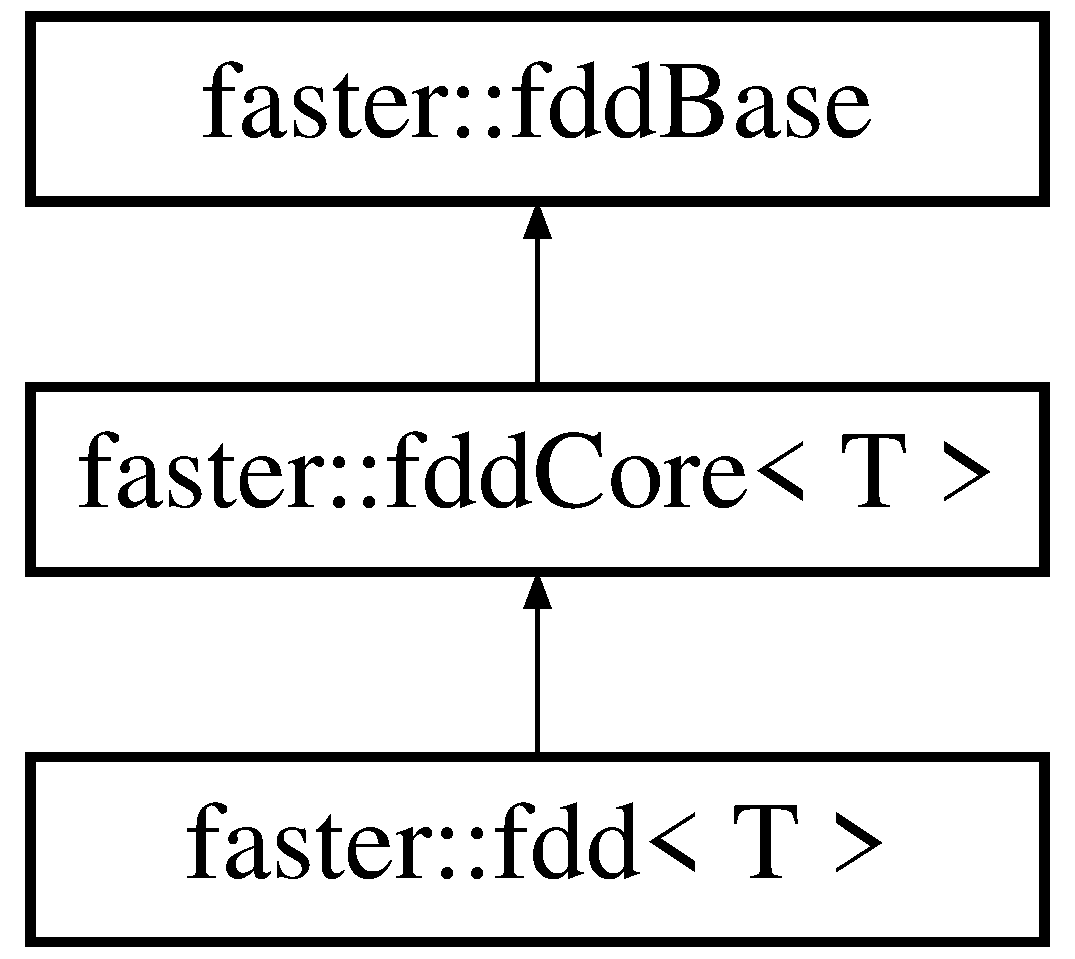
\includegraphics[height=3.000000cm]{classfaster_1_1fdd}
\end{center}
\end{figure}
\subsection*{Public Member Functions}
\begin{DoxyCompactItemize}
\item 
\hypertarget{classfaster_1_1fdd_a1f61fd1cb290f8d2f7570eb9f260866f}{}{\bfseries fdd} (\hyperlink{classfaster_1_1fastContext}{fast\+Context} \&c)\label{classfaster_1_1fdd_a1f61fd1cb290f8d2f7570eb9f260866f}

\item 
\hypertarget{classfaster_1_1fdd_a0ab5257609851930bd86b4de3094e8b4}{}{\bfseries fdd} (\hyperlink{classfaster_1_1fastContext}{fast\+Context} \&c, size\+\_\+t s, const std\+::vector$<$ size\+\_\+t $>$ \&data\+Alloc)\label{classfaster_1_1fdd_a0ab5257609851930bd86b4de3094e8b4}

\item 
\hypertarget{classfaster_1_1fdd_af37f3ee02b11f4e0c7b0cc9f0e241dee}{}{\bfseries fdd} (\hyperlink{classfaster_1_1fastContext}{fast\+Context} \&c, size\+\_\+t s)\label{classfaster_1_1fdd_af37f3ee02b11f4e0c7b0cc9f0e241dee}

\item 
\hypertarget{classfaster_1_1fdd_aa5b44359537e276d46a8902758501839}{}{\bfseries fdd} (\hyperlink{classfaster_1_1fastContext}{fast\+Context} \&c, T $\ast$data, size\+\_\+t size)\label{classfaster_1_1fdd_aa5b44359537e276d46a8902758501839}

\item 
\hypertarget{classfaster_1_1fdd_a76eee3a3adcb360d9b63bb50c1214de3}{}{\bfseries fdd} (\hyperlink{classfaster_1_1fastContext}{fast\+Context} \&c, std\+::vector$<$ T $>$ \&data\+V)\label{classfaster_1_1fdd_a76eee3a3adcb360d9b63bb50c1214de3}

\item 
\hypertarget{classfaster_1_1fdd_adc3ebc12c9d508b2957f5e6759544bee}{}{\bfseries fdd} (\hyperlink{classfaster_1_1fastContext}{fast\+Context} \&c, const char $\ast$file\+Name)\label{classfaster_1_1fdd_adc3ebc12c9d508b2957f5e6759544bee}

\item 
\hypertarget{classfaster_1_1fdd_a214d07df3240baf348492f9a4186d5cc}{}{\footnotesize template$<$typename U $>$ }\\\hyperlink{classfaster_1_1fdd}{fdd}$<$ U $>$ $\ast$ {\bfseries map} (map\+Function\+P$<$ T, U $>$ func\+P)\label{classfaster_1_1fdd_a214d07df3240baf348492f9a4186d5cc}

\item 
\hypertarget{classfaster_1_1fdd_a2cfde53328f21d2ffba58dde111219ff}{}{\footnotesize template$<$typename U $>$ }\\\hyperlink{classfaster_1_1fdd}{fdd}$<$ U $>$ $\ast$ {\bfseries map} (Pmap\+Function\+P$<$ T, U $>$ func\+P)\label{classfaster_1_1fdd_a2cfde53328f21d2ffba58dde111219ff}

\item 
\hypertarget{classfaster_1_1fdd_a17066a9f6526c2c630d730727c6b1b51}{}{\footnotesize template$<$typename L , typename U $>$ }\\\hyperlink{classfaster_1_1indexedFdd}{indexed\+Fdd}$<$ L, U $>$ $\ast$ {\bfseries map} (Imap\+Function\+P$<$ T, L, U $>$ func\+P)\label{classfaster_1_1fdd_a17066a9f6526c2c630d730727c6b1b51}

\item 
\hypertarget{classfaster_1_1fdd_a61ce985503e31026794696c6c6db20b8}{}{\footnotesize template$<$typename L , typename U $>$ }\\\hyperlink{classfaster_1_1indexedFdd}{indexed\+Fdd}$<$ L, U $>$ $\ast$ {\bfseries map} (I\+Pmap\+Function\+P$<$ T, L, U $>$ func\+P)\label{classfaster_1_1fdd_a61ce985503e31026794696c6c6db20b8}

\item 
\hypertarget{classfaster_1_1fdd_a0b4b82535fe1d2746973ce4e203d619f}{}{\footnotesize template$<$typename U $>$ }\\\hyperlink{classfaster_1_1fdd}{fdd}$<$ U $>$ $\ast$ {\bfseries bulk\+Map} (bulk\+Map\+Function\+P$<$ T, U $>$ func\+P)\label{classfaster_1_1fdd_a0b4b82535fe1d2746973ce4e203d619f}

\item 
\hypertarget{classfaster_1_1fdd_a72e07b032ee97aeed0261a20769720a7}{}{\footnotesize template$<$typename U $>$ }\\\hyperlink{classfaster_1_1fdd}{fdd}$<$ U $>$ $\ast$ {\bfseries bulk\+Map} (Pbulk\+Map\+Function\+P$<$ T, U $>$ func\+P)\label{classfaster_1_1fdd_a72e07b032ee97aeed0261a20769720a7}

\item 
\hypertarget{classfaster_1_1fdd_a97ad1e63823abe30de230da1456481d4}{}{\footnotesize template$<$typename L , typename U $>$ }\\\hyperlink{classfaster_1_1indexedFdd}{indexed\+Fdd}$<$ L, U $>$ $\ast$ {\bfseries bulk\+Map} (Ibulk\+Map\+Function\+P$<$ T, L, U $>$ func\+P)\label{classfaster_1_1fdd_a97ad1e63823abe30de230da1456481d4}

\item 
\hypertarget{classfaster_1_1fdd_abfd585e52364a7be20125aa25c0ab141}{}{\footnotesize template$<$typename L , typename U $>$ }\\\hyperlink{classfaster_1_1indexedFdd}{indexed\+Fdd}$<$ L, U $>$ $\ast$ {\bfseries bulk\+Map} (I\+Pbulk\+Map\+Function\+P$<$ T, L, U $>$ func\+P)\label{classfaster_1_1fdd_abfd585e52364a7be20125aa25c0ab141}

\item 
\hypertarget{classfaster_1_1fdd_a7efd43be1d3005d654c4656d521faf30}{}{\footnotesize template$<$typename U $>$ }\\\hyperlink{classfaster_1_1fdd}{fdd}$<$ U $>$ $\ast$ {\bfseries flat\+Map} (flat\+Map\+Function\+P$<$ T, U $>$ func\+P)\label{classfaster_1_1fdd_a7efd43be1d3005d654c4656d521faf30}

\item 
\hypertarget{classfaster_1_1fdd_a3f353414307512c23d88fc3e8b2e8221}{}{\footnotesize template$<$typename U $>$ }\\\hyperlink{classfaster_1_1fdd}{fdd}$<$ U $>$ $\ast$ {\bfseries flat\+Map} (Pflat\+Map\+Function\+P$<$ T, U $>$ func\+P)\label{classfaster_1_1fdd_a3f353414307512c23d88fc3e8b2e8221}

\item 
\hypertarget{classfaster_1_1fdd_a499a1c3638cc1e95e483cd91c7a884a7}{}{\footnotesize template$<$typename L , typename U $>$ }\\\hyperlink{classfaster_1_1indexedFdd}{indexed\+Fdd}$<$ L, U $>$ $\ast$ {\bfseries flat\+Map} (Iflat\+Map\+Function\+P$<$ T, L, U $>$ func\+P)\label{classfaster_1_1fdd_a499a1c3638cc1e95e483cd91c7a884a7}

\item 
\hypertarget{classfaster_1_1fdd_ab1c639e6fe55d66ac0cb50011d537567}{}{\footnotesize template$<$typename L , typename U $>$ }\\\hyperlink{classfaster_1_1indexedFdd}{indexed\+Fdd}$<$ L, U $>$ $\ast$ {\bfseries flat\+Map} (I\+Pflat\+Map\+Function\+P$<$ T, L, U $>$ func\+P)\label{classfaster_1_1fdd_ab1c639e6fe55d66ac0cb50011d537567}

\item 
\hypertarget{classfaster_1_1fdd_a6f87b4e650b28ea32c363f6d902babb1}{}{\footnotesize template$<$typename U $>$ }\\\hyperlink{classfaster_1_1fdd}{fdd}$<$ U $>$ $\ast$ {\bfseries bulk\+Flat\+Map} (bulk\+Flat\+Map\+Function\+P$<$ T, U $>$ func\+P)\label{classfaster_1_1fdd_a6f87b4e650b28ea32c363f6d902babb1}

\item 
\hypertarget{classfaster_1_1fdd_a77058c1365a8696105acaf1468e8d3b4}{}{\footnotesize template$<$typename U $>$ }\\\hyperlink{classfaster_1_1fdd}{fdd}$<$ U $>$ $\ast$ {\bfseries bulk\+Flat\+Map} (Pbulk\+Flat\+Map\+Function\+P$<$ T, U $>$ func\+P)\label{classfaster_1_1fdd_a77058c1365a8696105acaf1468e8d3b4}

\item 
\hypertarget{classfaster_1_1fdd_adfcb736f7161db476dbbb275f1d08659}{}{\footnotesize template$<$typename L , typename U $>$ }\\\hyperlink{classfaster_1_1indexedFdd}{indexed\+Fdd}$<$ L, U $>$ $\ast$ {\bfseries bulk\+Flat\+Map} (Ibulk\+Flat\+Map\+Function\+P$<$ T, L, U $>$ func\+P)\label{classfaster_1_1fdd_adfcb736f7161db476dbbb275f1d08659}

\item 
\hypertarget{classfaster_1_1fdd_af16d4811371f6dbcfbb717a73a182d48}{}{\footnotesize template$<$typename L , typename U $>$ }\\\hyperlink{classfaster_1_1indexedFdd}{indexed\+Fdd}$<$ L, U $>$ $\ast$ {\bfseries bulk\+Flat\+Map} (I\+Pbulk\+Flat\+Map\+Function\+P$<$ T, L, U $>$ func\+P)\label{classfaster_1_1fdd_af16d4811371f6dbcfbb717a73a182d48}

\item 
\hypertarget{classfaster_1_1fdd_a1e828ad9a768db382aef2adf878aa1b2}{}T {\bfseries reduce} (reduce\+Function\+P$<$ T $>$ func\+P)\label{classfaster_1_1fdd_a1e828ad9a768db382aef2adf878aa1b2}

\item 
\hypertarget{classfaster_1_1fdd_a8f133f23bd653329f44290ebda70bb9b}{}T {\bfseries bulk\+Reduce} (bulk\+Reduce\+Function\+P$<$ T $>$ func\+P)\label{classfaster_1_1fdd_a8f133f23bd653329f44290ebda70bb9b}

\item 
\hypertarget{classfaster_1_1fdd_a089aa4c91205948dacbc6e6bd6e5bcde}{}std\+::vector$<$ T $>$ {\bfseries collect} ()\label{classfaster_1_1fdd_a089aa4c91205948dacbc6e6bd6e5bcde}

\item 
\hypertarget{classfaster_1_1fdd_ac460ea12f02045a3d9203bb83eb5adb3}{}\hyperlink{classfaster_1_1fdd}{fdd}$<$ T $>$ $\ast$ {\bfseries cache} ()\label{classfaster_1_1fdd_ac460ea12f02045a3d9203bb83eb5adb3}

\end{DoxyCompactItemize}
\subsection*{Additional Inherited Members}


The documentation for this class was generated from the following files\+:\begin{DoxyCompactItemize}
\item 
/home/mtcs/pesquisa/faster/faster.\+git/src/include/fast\+Context.\+h\item 
/home/mtcs/pesquisa/faster/faster.\+git/src/include/fdd.\+h\end{DoxyCompactItemize}

\hypertarget{classfaster_1_1fdd_3_01T_01_5_01_4}{}\section{faster\+:\+:fdd$<$ T $\ast$ $>$ Class Template Reference}
\label{classfaster_1_1fdd_3_01T_01_5_01_4}\index{faster\+::fdd$<$ T $\ast$ $>$@{faster\+::fdd$<$ T $\ast$ $>$}}
Inheritance diagram for faster\+:\+:fdd$<$ T $\ast$ $>$\+:\begin{figure}[H]
\begin{center}
\leavevmode
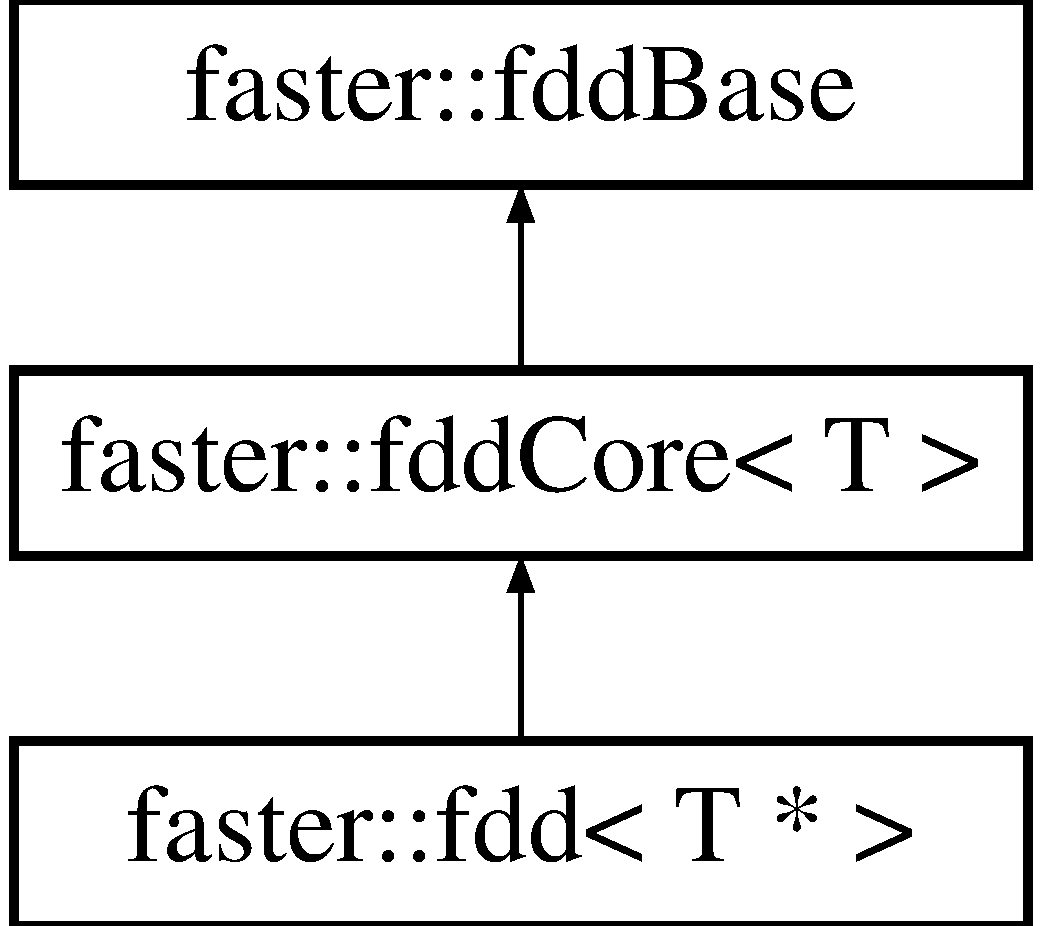
\includegraphics[height=3.000000cm]{classfaster_1_1fdd_3_01T_01_5_01_4}
\end{center}
\end{figure}
\subsection*{Public Member Functions}
\begin{DoxyCompactItemize}
\item 
\hypertarget{classfaster_1_1fdd_3_01T_01_5_01_4_a5e4ef770313ef0061b7039102463d1bb}{}{\bfseries fdd} (\hyperlink{classfaster_1_1fastContext}{fast\+Context} \&c)\label{classfaster_1_1fdd_3_01T_01_5_01_4_a5e4ef770313ef0061b7039102463d1bb}

\item 
\hypertarget{classfaster_1_1fdd_3_01T_01_5_01_4_aeff7da6018786d1e58fefc80a04e0f41}{}{\bfseries fdd} (\hyperlink{classfaster_1_1fastContext}{fast\+Context} \&c, size\+\_\+t s, const std\+::vector$<$ size\+\_\+t $>$ \&data\+Alloc)\label{classfaster_1_1fdd_3_01T_01_5_01_4_aeff7da6018786d1e58fefc80a04e0f41}

\item 
\hypertarget{classfaster_1_1fdd_3_01T_01_5_01_4_aeece4f42b6eff6fef26a0c0fe9fc88fa}{}{\bfseries fdd} (\hyperlink{classfaster_1_1fastContext}{fast\+Context} \&c, size\+\_\+t s)\label{classfaster_1_1fdd_3_01T_01_5_01_4_aeece4f42b6eff6fef26a0c0fe9fc88fa}

\item 
\hypertarget{classfaster_1_1fdd_3_01T_01_5_01_4_ab844e7f258c74838fb468214325b50d6}{}{\bfseries fdd} (\hyperlink{classfaster_1_1fastContext}{fast\+Context} \&c, T $\ast$data\mbox{[}$\,$\mbox{]}, size\+\_\+t data\+Sizes\mbox{[}$\,$\mbox{]}, size\+\_\+t size)\label{classfaster_1_1fdd_3_01T_01_5_01_4_ab844e7f258c74838fb468214325b50d6}

\item 
\hypertarget{classfaster_1_1fdd_3_01T_01_5_01_4_ad3d34fd674c74c0d78b771c8b66c1597}{}{\footnotesize template$<$typename U $>$ }\\\hyperlink{classfaster_1_1fdd}{fdd}$<$ U $>$ $\ast$ {\bfseries map} (map\+P\+Function\+P$<$ T, U $>$ func\+P)\label{classfaster_1_1fdd_3_01T_01_5_01_4_ad3d34fd674c74c0d78b771c8b66c1597}

\item 
\hypertarget{classfaster_1_1fdd_3_01T_01_5_01_4_a7c80a0dbb77a88c1c6158c8516b4c698}{}{\footnotesize template$<$typename U $>$ }\\\hyperlink{classfaster_1_1fdd}{fdd}$<$ U $>$ $\ast$ {\bfseries map} (Pmap\+P\+Function\+P$<$ T, U $>$ func\+P)\label{classfaster_1_1fdd_3_01T_01_5_01_4_a7c80a0dbb77a88c1c6158c8516b4c698}

\item 
\hypertarget{classfaster_1_1fdd_3_01T_01_5_01_4_a56cd3496f7b7e836af3df5a511d2b3d7}{}{\footnotesize template$<$typename L , typename U $>$ }\\\hyperlink{classfaster_1_1indexedFdd}{indexed\+Fdd}$<$ L, U $>$ $\ast$ {\bfseries map} (Imap\+P\+Function\+P$<$ T, L, U $>$ func\+P)\label{classfaster_1_1fdd_3_01T_01_5_01_4_a56cd3496f7b7e836af3df5a511d2b3d7}

\item 
\hypertarget{classfaster_1_1fdd_3_01T_01_5_01_4_ae2c6b56f97e260ada3f6115f7dc852ac}{}{\footnotesize template$<$typename L , typename U $>$ }\\\hyperlink{classfaster_1_1indexedFdd}{indexed\+Fdd}$<$ L, U $>$ $\ast$ {\bfseries map} (I\+Pmap\+P\+Function\+P$<$ T, L, U $>$ func\+P)\label{classfaster_1_1fdd_3_01T_01_5_01_4_ae2c6b56f97e260ada3f6115f7dc852ac}

\item 
\hypertarget{classfaster_1_1fdd_3_01T_01_5_01_4_abbf7abb6ecd34cf25150dd10cbc1ad09}{}{\footnotesize template$<$typename U $>$ }\\\hyperlink{classfaster_1_1fdd}{fdd}$<$ U $>$ $\ast$ {\bfseries bulk\+Map} (bulk\+Map\+P\+Function\+P$<$ T, U $>$ func\+P)\label{classfaster_1_1fdd_3_01T_01_5_01_4_abbf7abb6ecd34cf25150dd10cbc1ad09}

\item 
\hypertarget{classfaster_1_1fdd_3_01T_01_5_01_4_a25acd0d4b8ef01f7a60b17ff33024160}{}{\footnotesize template$<$typename U $>$ }\\\hyperlink{classfaster_1_1fdd}{fdd}$<$ U $>$ $\ast$ {\bfseries bulk\+Map} (Pbulk\+Map\+P\+Function\+P$<$ T, U $>$ func\+P)\label{classfaster_1_1fdd_3_01T_01_5_01_4_a25acd0d4b8ef01f7a60b17ff33024160}

\item 
\hypertarget{classfaster_1_1fdd_3_01T_01_5_01_4_ae4d426d09264286ae02c1aa0bf9356e2}{}{\footnotesize template$<$typename L , typename U $>$ }\\\hyperlink{classfaster_1_1indexedFdd}{indexed\+Fdd}$<$ L, U $>$ $\ast$ {\bfseries bulk\+Map} (Ibulk\+Map\+P\+Function\+P$<$ T, L, U $>$ func\+P)\label{classfaster_1_1fdd_3_01T_01_5_01_4_ae4d426d09264286ae02c1aa0bf9356e2}

\item 
\hypertarget{classfaster_1_1fdd_3_01T_01_5_01_4_ac83f6ce9ca84f55c4ad8dc2f8f0fcad7}{}{\footnotesize template$<$typename L , typename U $>$ }\\\hyperlink{classfaster_1_1indexedFdd}{indexed\+Fdd}$<$ L, U $>$ $\ast$ {\bfseries bulk\+Map} (I\+Pbulk\+Map\+P\+Function\+P$<$ T, L, U $>$ func\+P)\label{classfaster_1_1fdd_3_01T_01_5_01_4_ac83f6ce9ca84f55c4ad8dc2f8f0fcad7}

\item 
\hypertarget{classfaster_1_1fdd_3_01T_01_5_01_4_af490d108ce1a30dc4210a1d8b557df97}{}{\footnotesize template$<$typename U $>$ }\\\hyperlink{classfaster_1_1fdd}{fdd}$<$ U $>$ $\ast$ {\bfseries flat\+Map} (flat\+Map\+P\+Function\+P$<$ T, U $>$ func\+P)\label{classfaster_1_1fdd_3_01T_01_5_01_4_af490d108ce1a30dc4210a1d8b557df97}

\item 
\hypertarget{classfaster_1_1fdd_3_01T_01_5_01_4_a5fad18905c1f51701c823959d520b075}{}{\footnotesize template$<$typename U $>$ }\\\hyperlink{classfaster_1_1fdd}{fdd}$<$ U $>$ $\ast$ {\bfseries flat\+Map} (Pflat\+Map\+P\+Function\+P$<$ T, U $>$ func\+P)\label{classfaster_1_1fdd_3_01T_01_5_01_4_a5fad18905c1f51701c823959d520b075}

\item 
\hypertarget{classfaster_1_1fdd_3_01T_01_5_01_4_a03c1134e4e6770f0dad78d073ad36c48}{}{\footnotesize template$<$typename L , typename U $>$ }\\\hyperlink{classfaster_1_1indexedFdd}{indexed\+Fdd}$<$ L, U $>$ $\ast$ {\bfseries flat\+Map} (Iflat\+Map\+P\+Function\+P$<$ T, L, U $>$ func\+P)\label{classfaster_1_1fdd_3_01T_01_5_01_4_a03c1134e4e6770f0dad78d073ad36c48}

\item 
\hypertarget{classfaster_1_1fdd_3_01T_01_5_01_4_a4d183f4e1d6545769022d805a2d841f6}{}{\footnotesize template$<$typename L , typename U $>$ }\\\hyperlink{classfaster_1_1indexedFdd}{indexed\+Fdd}$<$ L, U $>$ $\ast$ {\bfseries flat\+Map} (I\+Pflat\+Map\+P\+Function\+P$<$ T, L, U $>$ func\+P)\label{classfaster_1_1fdd_3_01T_01_5_01_4_a4d183f4e1d6545769022d805a2d841f6}

\item 
\hypertarget{classfaster_1_1fdd_3_01T_01_5_01_4_a7519a944f8bef5f27466d341f39bbb0e}{}{\footnotesize template$<$typename U $>$ }\\\hyperlink{classfaster_1_1fdd}{fdd}$<$ U $>$ $\ast$ {\bfseries bulk\+Flat\+Map} (bulk\+Flat\+Map\+P\+Function\+P$<$ T, U $>$ func\+P)\label{classfaster_1_1fdd_3_01T_01_5_01_4_a7519a944f8bef5f27466d341f39bbb0e}

\item 
\hypertarget{classfaster_1_1fdd_3_01T_01_5_01_4_a91e2f6a811a43d36a26e022d92704b3f}{}{\footnotesize template$<$typename U $>$ }\\\hyperlink{classfaster_1_1fdd}{fdd}$<$ U $>$ $\ast$ {\bfseries bulk\+Flat\+Map} (Pbulk\+Flat\+Map\+P\+Function\+P$<$ T, U $>$ func\+P)\label{classfaster_1_1fdd_3_01T_01_5_01_4_a91e2f6a811a43d36a26e022d92704b3f}

\item 
\hypertarget{classfaster_1_1fdd_3_01T_01_5_01_4_ac930844af424e4434920531d285addaf}{}{\footnotesize template$<$typename L , typename U $>$ }\\\hyperlink{classfaster_1_1indexedFdd}{indexed\+Fdd}$<$ L, U $>$ $\ast$ {\bfseries bulk\+Flat\+Map} (Ibulk\+Flat\+Map\+P\+Function\+P$<$ T, L, U $>$ func\+P)\label{classfaster_1_1fdd_3_01T_01_5_01_4_ac930844af424e4434920531d285addaf}

\item 
\hypertarget{classfaster_1_1fdd_3_01T_01_5_01_4_a9215f59e778be75025275ee5954beacb}{}{\footnotesize template$<$typename L , typename U $>$ }\\\hyperlink{classfaster_1_1indexedFdd}{indexed\+Fdd}$<$ L, U $>$ $\ast$ {\bfseries bulk\+Flat\+Map} (I\+Pbulk\+Flat\+Map\+P\+Function\+P$<$ T, L, U $>$ func\+P)\label{classfaster_1_1fdd_3_01T_01_5_01_4_a9215f59e778be75025275ee5954beacb}

\item 
\hypertarget{classfaster_1_1fdd_3_01T_01_5_01_4_a14f17acd4d8412255e0b075d51f04a3f}{}std\+::vector$<$ T $>$ {\bfseries reduce} (Preduce\+P\+Function\+P$<$ T $>$ func\+P)\label{classfaster_1_1fdd_3_01T_01_5_01_4_a14f17acd4d8412255e0b075d51f04a3f}

\item 
\hypertarget{classfaster_1_1fdd_3_01T_01_5_01_4_a95830370065eb3bd41ea93b7843199be}{}std\+::vector$<$ T $>$ {\bfseries bulk\+Reduce} (Pbulk\+Reduce\+P\+Function\+P$<$ T $>$ func\+P)\label{classfaster_1_1fdd_3_01T_01_5_01_4_a95830370065eb3bd41ea93b7843199be}

\item 
\hypertarget{classfaster_1_1fdd_3_01T_01_5_01_4_aa2e17d79b0f34c2722f9502b8ca56d29}{}std\+::vector$<$ std\+::pair$<$ T $\ast$, size\+\_\+t $>$ $>$ {\bfseries collect} ()\label{classfaster_1_1fdd_3_01T_01_5_01_4_aa2e17d79b0f34c2722f9502b8ca56d29}

\item 
\hypertarget{classfaster_1_1fdd_3_01T_01_5_01_4_a819ca1aeeee4808b7c19a7d30d3be249}{}\hyperlink{classfaster_1_1fdd}{fdd}$<$ T $\ast$ $>$ $\ast$ {\bfseries cache} ()\label{classfaster_1_1fdd_3_01T_01_5_01_4_a819ca1aeeee4808b7c19a7d30d3be249}

\end{DoxyCompactItemize}
\subsection*{Additional Inherited Members}


The documentation for this class was generated from the following file\+:\begin{DoxyCompactItemize}
\item 
/home/mtcs/pesquisa/faster/faster.\+git/src/include/fdd.\+h\end{DoxyCompactItemize}

\hypertarget{classfaster_1_1fddBase}{}\section{faster\+:\+:fdd\+Base Class Reference}
\label{classfaster_1_1fddBase}\index{faster\+::fdd\+Base@{faster\+::fdd\+Base}}
Inheritance diagram for faster\+:\+:fdd\+Base\+:\begin{figure}[H]
\begin{center}
\leavevmode
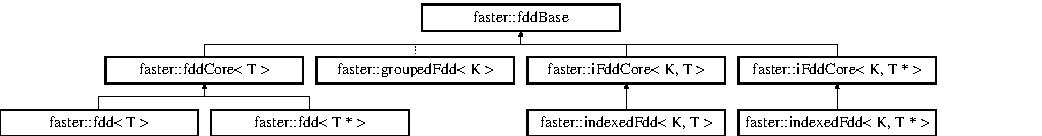
\includegraphics[height=1.826087cm]{classfaster_1_1fddBase}
\end{center}
\end{figure}
\subsection*{Public Member Functions}
\begin{DoxyCompactItemize}
\item 
\hypertarget{classfaster_1_1fddBase_a41699519e9774d380bd0053f3d3b995a}{}void {\bfseries set\+Size} (size\+\_\+t \&s)\label{classfaster_1_1fddBase_a41699519e9774d380bd0053f3d3b995a}

\item 
\hypertarget{classfaster_1_1fddBase_ab9645c31245a53f97449446a440adf47}{}size\+\_\+t {\bfseries get\+Size} ()\label{classfaster_1_1fddBase_ab9645c31245a53f97449446a440adf47}

\item 
\hypertarget{classfaster_1_1fddBase_a3902296c393cb15e830c02555a0f371f}{}int {\bfseries get\+Id} ()\label{classfaster_1_1fddBase_a3902296c393cb15e830c02555a0f371f}

\item 
\hypertarget{classfaster_1_1fddBase_a2b6f4b4fa670e90cde938d456e5da3b7}{}const std\+::vector$<$ size\+\_\+t $>$ \& {\bfseries get\+Alloc} ()\label{classfaster_1_1fddBase_a2b6f4b4fa670e90cde938d456e5da3b7}

\item 
\hypertarget{classfaster_1_1fddBase_a640157513b4752863e877391de92ede4}{}fdd\+Type {\bfseries t\+Type} ()\label{classfaster_1_1fddBase_a640157513b4752863e877391de92ede4}

\item 
\hypertarget{classfaster_1_1fddBase_a18c8bafa38afa84895db3c27c0416187}{}fdd\+Type {\bfseries k\+Type} ()\label{classfaster_1_1fddBase_a18c8bafa38afa84895db3c27c0416187}

\item 
\hypertarget{classfaster_1_1fddBase_ae2b4fdf3a1e7ac336b21f5e197dfb4a7}{}bool {\bfseries is\+Cached} ()\label{classfaster_1_1fddBase_ae2b4fdf3a1e7ac336b21f5e197dfb4a7}

\item 
\hypertarget{classfaster_1_1fddBase_a4cbed7c20357b0732414af58a9d60380}{}virtual void {\bfseries discard} ()=0\label{classfaster_1_1fddBase_a4cbed7c20357b0732414af58a9d60380}

\item 
\hypertarget{classfaster_1_1fddBase_a63b8a060663ac590bc83fa676fef74f4}{}virtual void $\ast$ {\bfseries get\+Key\+Map} (void)=0\label{classfaster_1_1fddBase_a63b8a060663ac590bc83fa676fef74f4}

\item 
\hypertarget{classfaster_1_1fddBase_ab36e7bd326034eca0721347b2a5b1bfe}{}virtual void {\bfseries set\+Key\+Map} (void $\ast$key\+Map)=0\label{classfaster_1_1fddBase_ab36e7bd326034eca0721347b2a5b1bfe}

\item 
\hypertarget{classfaster_1_1fddBase_a14ec9acc33546362f86ac34b369956fa}{}virtual bool {\bfseries is\+Grouped\+By\+Key} ()=0\label{classfaster_1_1fddBase_a14ec9acc33546362f86ac34b369956fa}

\item 
\hypertarget{classfaster_1_1fddBase_a0758eda48ad1cee20071ba8ce1852037}{}virtual void {\bfseries set\+Grouped\+By\+Key} (bool gbk)=0\label{classfaster_1_1fddBase_a0758eda48ad1cee20071ba8ce1852037}

\end{DoxyCompactItemize}
\subsection*{Protected Attributes}
\begin{DoxyCompactItemize}
\item 
\hypertarget{classfaster_1_1fddBase_a585bdd9659c1ab92cf615c73fc4d9ac7}{}fdd\+Type {\bfseries \+\_\+k\+Type}\label{classfaster_1_1fddBase_a585bdd9659c1ab92cf615c73fc4d9ac7}

\item 
\hypertarget{classfaster_1_1fddBase_a7ee5fc280f8eed2ffe97ef9c7a8b0919}{}fdd\+Type {\bfseries \+\_\+t\+Type}\label{classfaster_1_1fddBase_a7ee5fc280f8eed2ffe97ef9c7a8b0919}

\item 
\hypertarget{classfaster_1_1fddBase_a6ebf1389a80e31abed31f5b85d99fa1a}{}unsigned long int {\bfseries id}\label{classfaster_1_1fddBase_a6ebf1389a80e31abed31f5b85d99fa1a}

\item 
\hypertarget{classfaster_1_1fddBase_ac69c521f69cbe163b676f7723c9dd024}{}unsigned long int {\bfseries total\+Blocks}\label{classfaster_1_1fddBase_ac69c521f69cbe163b676f7723c9dd024}

\item 
\hypertarget{classfaster_1_1fddBase_a397adc12ccc9f7eccce83dfef625487c}{}unsigned long int {\bfseries size}\label{classfaster_1_1fddBase_a397adc12ccc9f7eccce83dfef625487c}

\item 
\hypertarget{classfaster_1_1fddBase_a47961f2f165f2e148d9cbbd1b59090d3}{}std\+::vector$<$ size\+\_\+t $>$ {\bfseries data\+Alloc}\label{classfaster_1_1fddBase_a47961f2f165f2e148d9cbbd1b59090d3}

\item 
\hypertarget{classfaster_1_1fddBase_acd5a472da183f35b13197804acadac4e}{}bool {\bfseries cached}\label{classfaster_1_1fddBase_acd5a472da183f35b13197804acadac4e}

\end{DoxyCompactItemize}


The documentation for this class was generated from the following file\+:\begin{DoxyCompactItemize}
\item 
/home/mtcs/pesquisa/faster/faster.\+git/src/include/fdd\+Base.\+h\end{DoxyCompactItemize}

\hypertarget{classfaster_1_1fddCore}{}\section{faster\+:\+:fdd\+Core$<$ T $>$ Class Template Reference}
\label{classfaster_1_1fddCore}\index{faster\+::fdd\+Core$<$ T $>$@{faster\+::fdd\+Core$<$ T $>$}}
Inheritance diagram for faster\+:\+:fdd\+Core$<$ T $>$\+:\begin{figure}[H]
\begin{center}
\leavevmode
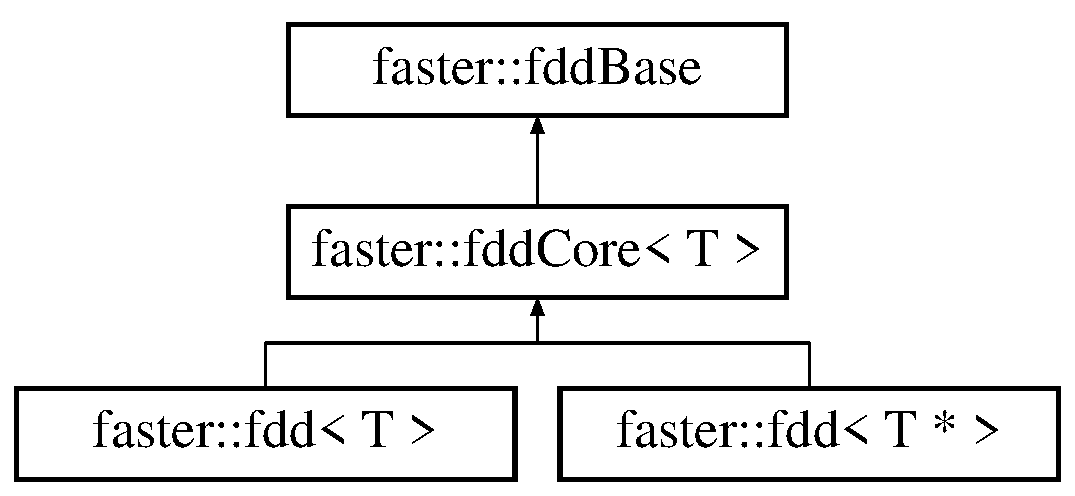
\includegraphics[height=3.000000cm]{classfaster_1_1fddCore}
\end{center}
\end{figure}
\subsection*{Public Member Functions}
\begin{DoxyCompactItemize}
\item 
\hypertarget{classfaster_1_1fddCore_a0addecf1c27311b6da3e37f77e414572}{}void {\bfseries discard} ()\label{classfaster_1_1fddCore_a0addecf1c27311b6da3e37f77e414572}

\item 
\hypertarget{classfaster_1_1fddCore_a7dcd1b146c23c5f5ba149a6fc2bc7741}{}void $\ast$ {\bfseries get\+Key\+Map} ()\label{classfaster_1_1fddCore_a7dcd1b146c23c5f5ba149a6fc2bc7741}

\item 
\hypertarget{classfaster_1_1fddCore_ae268b85e9f217e3942600c11b8aa3347}{}void {\bfseries set\+Key\+Map} (void $\ast$key\+Map U\+N\+U\+S\+E\+D)\label{classfaster_1_1fddCore_ae268b85e9f217e3942600c11b8aa3347}

\item 
\hypertarget{classfaster_1_1fddCore_a4ff77df4fb389f5ee6ff468f773d58f8}{}bool {\bfseries is\+Grouped\+By\+Key} ()\label{classfaster_1_1fddCore_a4ff77df4fb389f5ee6ff468f773d58f8}

\item 
\hypertarget{classfaster_1_1fddCore_a9a47c562a1f92f6c7f79968beb339c3d}{}void {\bfseries set\+Grouped\+By\+Key} (bool gbk U\+N\+U\+S\+E\+D)\label{classfaster_1_1fddCore_a9a47c562a1f92f6c7f79968beb339c3d}

\end{DoxyCompactItemize}
\subsection*{Protected Member Functions}
\begin{DoxyCompactItemize}
\item 
\hypertarget{classfaster_1_1fddCore_af2bf966f3d75e2d7d0d81f120fb7599a}{}{\bfseries fdd\+Core} (\hyperlink{classfaster_1_1fastContext}{fast\+Context} \&c)\label{classfaster_1_1fddCore_af2bf966f3d75e2d7d0d81f120fb7599a}

\item 
\hypertarget{classfaster_1_1fddCore_a437156da84fb4f0e7cb58f2f67ff172b}{}{\bfseries fdd\+Core} (\hyperlink{classfaster_1_1fastContext}{fast\+Context} \&c, size\+\_\+t s, const std\+::vector$<$ size\+\_\+t $>$ \&data\+Alloc)\label{classfaster_1_1fddCore_a437156da84fb4f0e7cb58f2f67ff172b}

\item 
\hypertarget{classfaster_1_1fddCore_a1fff34f140b7634b1a6e60b8069a3a29}{}\hyperlink{classfaster_1_1fddBase}{fdd\+Base} $\ast$ {\bfseries \+\_\+map} (void $\ast$func\+P, fdd\+Op\+Type op, \hyperlink{classfaster_1_1fddBase}{fdd\+Base} $\ast$new\+Fdd)\label{classfaster_1_1fddCore_a1fff34f140b7634b1a6e60b8069a3a29}

\item 
\hypertarget{classfaster_1_1fddCore_a87e8b9e76ef7138a1394265528944ffe}{}{\footnotesize template$<$typename L , typename U $>$ }\\\hyperlink{classfaster_1_1indexedFdd}{indexed\+Fdd}$<$ L, U $>$ $\ast$ {\bfseries map\+I} (void $\ast$func\+P, fdd\+Op\+Type op)\label{classfaster_1_1fddCore_a87e8b9e76ef7138a1394265528944ffe}

\item 
\hypertarget{classfaster_1_1fddCore_a30e174ccee6fc2d00387c85161422825}{}{\footnotesize template$<$typename U $>$ }\\\hyperlink{classfaster_1_1fdd}{fdd}$<$ U $>$ $\ast$ {\bfseries map} (void $\ast$func\+P, fdd\+Op\+Type op)\label{classfaster_1_1fddCore_a30e174ccee6fc2d00387c85161422825}

\end{DoxyCompactItemize}
\subsection*{Protected Attributes}
\begin{DoxyCompactItemize}
\item 
\hypertarget{classfaster_1_1fddCore_aa2bf63bd5c77afe78061ed4df3713a76}{}\hyperlink{classfaster_1_1fastContext}{fast\+Context} $\ast$ {\bfseries context}\label{classfaster_1_1fddCore_aa2bf63bd5c77afe78061ed4df3713a76}

\end{DoxyCompactItemize}


The documentation for this class was generated from the following file\+:\begin{DoxyCompactItemize}
\item 
/home/mtcs/pesquisa/faster/faster.\+git/src/include/fdd.\+h\end{DoxyCompactItemize}

\hypertarget{classfaster_1_1fddStorage}{}\section{faster\+:\+:fdd\+Storage$<$ T $>$ Class Template Reference}
\label{classfaster_1_1fddStorage}\index{faster\+::fdd\+Storage$<$ T $>$@{faster\+::fdd\+Storage$<$ T $>$}}
Inheritance diagram for faster\+:\+:fdd\+Storage$<$ T $>$\+:\begin{figure}[H]
\begin{center}
\leavevmode
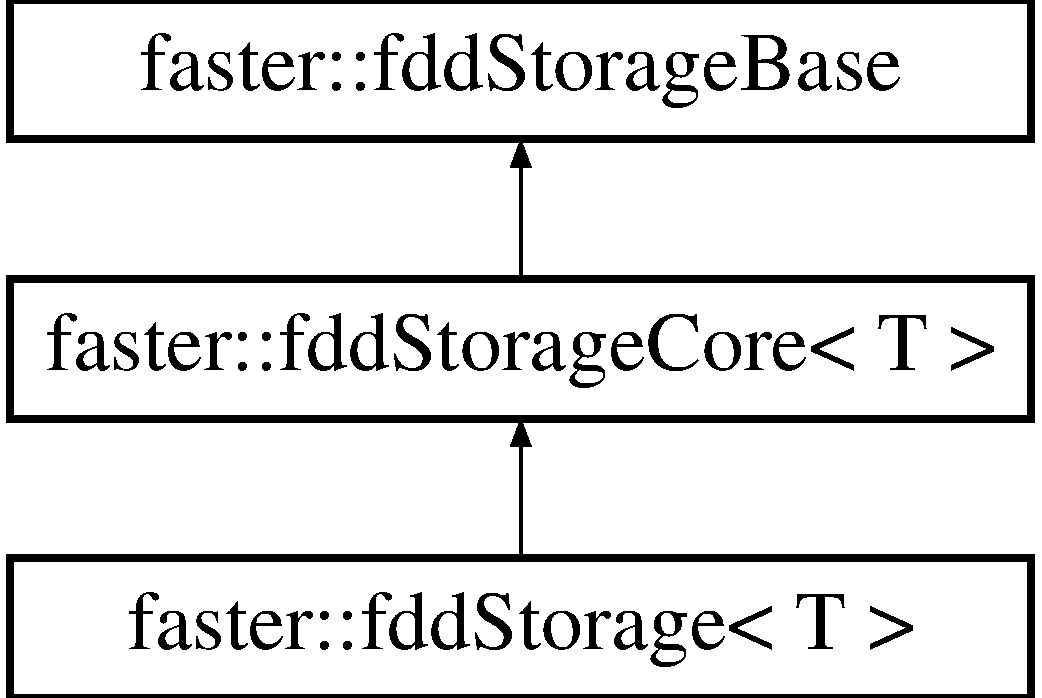
\includegraphics[height=3.000000cm]{classfaster_1_1fddStorage}
\end{center}
\end{figure}
\subsection*{Public Member Functions}
\begin{DoxyCompactItemize}
\item 
\hypertarget{classfaster_1_1fddStorage_a64a6657ec7779098209f214e9eb0dcbf}{}{\bfseries fdd\+Storage} (size\+\_\+t s)\label{classfaster_1_1fddStorage_a64a6657ec7779098209f214e9eb0dcbf}

\item 
\hypertarget{classfaster_1_1fddStorage_ac559d1855128c84e2afecad11e6c544e}{}{\bfseries fdd\+Storage} (T $\ast$data, size\+\_\+t s)\label{classfaster_1_1fddStorage_ac559d1855128c84e2afecad11e6c544e}

\item 
\hypertarget{classfaster_1_1fddStorage_ab766932e5707c5e89811848024e4d8ca}{}void {\bfseries set\+Data} (T $\ast$data, size\+\_\+t s)\label{classfaster_1_1fddStorage_ab766932e5707c5e89811848024e4d8ca}

\item 
\hypertarget{classfaster_1_1fddStorage_aae86c7f166895c3bcb4da4dfd0029856}{}void {\bfseries set\+Data\+Raw} (void $\ast$data, size\+\_\+t s)\label{classfaster_1_1fddStorage_aae86c7f166895c3bcb4da4dfd0029856}

\item 
\hypertarget{classfaster_1_1fddStorage_a11e678410ee62756860b55073d89ee2f}{}void {\bfseries set\+Size} (size\+\_\+t s) override\label{classfaster_1_1fddStorage_a11e678410ee62756860b55073d89ee2f}

\item 
\hypertarget{classfaster_1_1fddStorage_aae02a1cfeb1845ab9f7e347fbafcb791}{}void {\bfseries insert} (T \&item)\label{classfaster_1_1fddStorage_aae02a1cfeb1845ab9f7e347fbafcb791}

\item 
\hypertarget{classfaster_1_1fddStorage_aa0e4fd7ae90d85ff2f1b4654c2bf0960}{}void {\bfseries grow} (size\+\_\+t to\+Size)\label{classfaster_1_1fddStorage_aa0e4fd7ae90d85ff2f1b4654c2bf0960}

\item 
\hypertarget{classfaster_1_1fddStorage_a919925ed678dad9b556d9cdc4974d4a9}{}void {\bfseries shrink} ()\label{classfaster_1_1fddStorage_a919925ed678dad9b556d9cdc4974d4a9}

\end{DoxyCompactItemize}
\subsection*{Additional Inherited Members}


The documentation for this class was generated from the following files\+:\begin{DoxyCompactItemize}
\item 
/home/mtcs/pesquisa/faster/faster.\+git/src/include/\+\_\+worker\+Fdd.\+h\item 
/home/mtcs/pesquisa/faster/faster.\+git/src/include/fdd\+Storage.\+h\item 
/home/mtcs/pesquisa/faster/faster.\+git/src/libfaster/fdd\+Storage.\+cpp\end{DoxyCompactItemize}

\hypertarget{classfaster_1_1fddStorage_3_01T_01_5_01_4}{}\section{faster\+:\+:fdd\+Storage$<$ T $\ast$ $>$ Class Template Reference}
\label{classfaster_1_1fddStorage_3_01T_01_5_01_4}\index{faster\+::fdd\+Storage$<$ T $\ast$ $>$@{faster\+::fdd\+Storage$<$ T $\ast$ $>$}}
Inheritance diagram for faster\+:\+:fdd\+Storage$<$ T $\ast$ $>$\+:\begin{figure}[H]
\begin{center}
\leavevmode
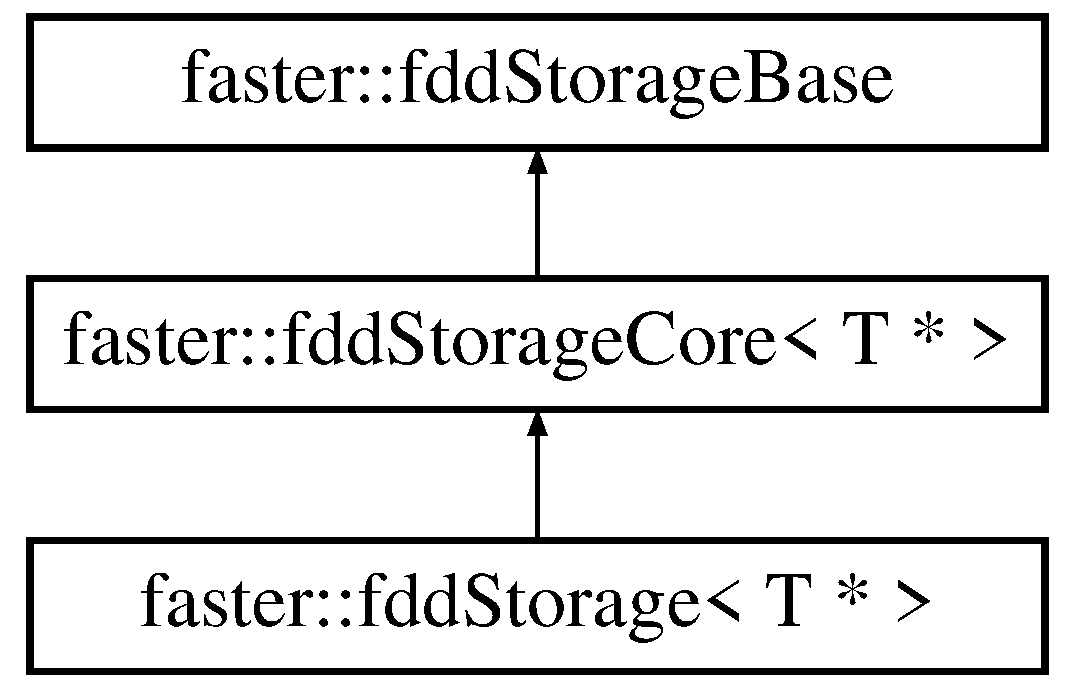
\includegraphics[height=3.000000cm]{classfaster_1_1fddStorage_3_01T_01_5_01_4}
\end{center}
\end{figure}
\subsection*{Public Member Functions}
\begin{DoxyCompactItemize}
\item 
\hypertarget{classfaster_1_1fddStorage_3_01T_01_5_01_4_a949dbdd099a0dc2b54cec12cfb3f21b0}{}{\bfseries fdd\+Storage} (size\+\_\+t s)\label{classfaster_1_1fddStorage_3_01T_01_5_01_4_a949dbdd099a0dc2b54cec12cfb3f21b0}

\item 
\hypertarget{classfaster_1_1fddStorage_3_01T_01_5_01_4_a6272c1fb1e8bdff3c70f8fbe46c90fc4}{}{\bfseries fdd\+Storage} (T $\ast$$\ast$data, size\+\_\+t $\ast$line\+Sizes, size\+\_\+t s)\label{classfaster_1_1fddStorage_3_01T_01_5_01_4_a6272c1fb1e8bdff3c70f8fbe46c90fc4}

\item 
\hypertarget{classfaster_1_1fddStorage_3_01T_01_5_01_4_a4835be07a5ec230490f03da7cb8e3e16}{}void {\bfseries set\+Data} (T $\ast$$\ast$data, size\+\_\+t $\ast$line\+Sizes, size\+\_\+t s)\label{classfaster_1_1fddStorage_3_01T_01_5_01_4_a4835be07a5ec230490f03da7cb8e3e16}

\item 
\hypertarget{classfaster_1_1fddStorage_3_01T_01_5_01_4_aeb87efbfa61cc52dfc3bbdc3d09408dd}{}void {\bfseries set\+Data\+Raw} (void $\ast$data, size\+\_\+t $\ast$line\+Sizes, size\+\_\+t s)\label{classfaster_1_1fddStorage_3_01T_01_5_01_4_aeb87efbfa61cc52dfc3bbdc3d09408dd}

\item 
\hypertarget{classfaster_1_1fddStorage_3_01T_01_5_01_4_a5a918f95b08ed5a81fbb8831b0fc196e}{}void {\bfseries set\+Size} (size\+\_\+t s) override\label{classfaster_1_1fddStorage_3_01T_01_5_01_4_a5a918f95b08ed5a81fbb8831b0fc196e}

\item 
\hypertarget{classfaster_1_1fddStorage_3_01T_01_5_01_4_ae6b278b0a9dc5a96821438f0fb667489}{}void {\bfseries insert} (T $\ast$\&item, size\+\_\+t s)\label{classfaster_1_1fddStorage_3_01T_01_5_01_4_ae6b278b0a9dc5a96821438f0fb667489}

\item 
\hypertarget{classfaster_1_1fddStorage_3_01T_01_5_01_4_a44e871ff8dcd4b40f379330a78b6056a}{}size\+\_\+t $\ast$ {\bfseries get\+Line\+Sizes} ()\label{classfaster_1_1fddStorage_3_01T_01_5_01_4_a44e871ff8dcd4b40f379330a78b6056a}

\item 
\hypertarget{classfaster_1_1fddStorage_3_01T_01_5_01_4_a76493eba9895f152a95b547a2485bc3a}{}void {\bfseries grow} (size\+\_\+t to\+Size)\label{classfaster_1_1fddStorage_3_01T_01_5_01_4_a76493eba9895f152a95b547a2485bc3a}

\item 
\hypertarget{classfaster_1_1fddStorage_3_01T_01_5_01_4_adac945484d94be1469e4cf9eb6e8c16c}{}void {\bfseries shrink} ()\label{classfaster_1_1fddStorage_3_01T_01_5_01_4_adac945484d94be1469e4cf9eb6e8c16c}

\end{DoxyCompactItemize}
\subsection*{Additional Inherited Members}


The documentation for this class was generated from the following files\+:\begin{DoxyCompactItemize}
\item 
/home/mtcs/pesquisa/faster/faster.\+git/src/include/fdd\+Storage.\+h\item 
/home/mtcs/pesquisa/faster/faster.\+git/src/libfaster/fdd\+Storage.\+cpp\end{DoxyCompactItemize}

\hypertarget{classfaster_1_1fddStorageBase}{}\section{faster\+:\+:fdd\+Storage\+Base Class Reference}
\label{classfaster_1_1fddStorageBase}\index{faster\+::fdd\+Storage\+Base@{faster\+::fdd\+Storage\+Base}}
Inheritance diagram for faster\+:\+:fdd\+Storage\+Base\+:\begin{figure}[H]
\begin{center}
\leavevmode
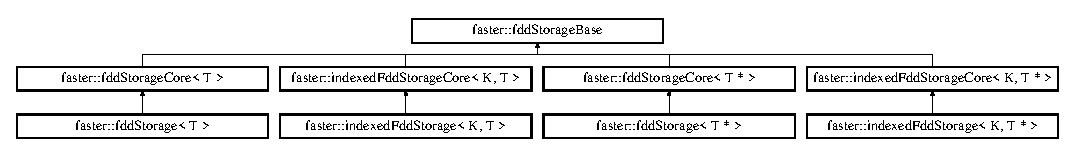
\includegraphics[height=1.093750cm]{classfaster_1_1fddStorageBase}
\end{center}
\end{figure}


\subsection{Description}
\subsection*{Public Member Functions}
\begin{DoxyCompactItemize}
\item 
\hypertarget{classfaster_1_1fddStorageBase_a8052833a8e5c933d14370c0c3ed6bdeb}{}\label{classfaster_1_1fddStorageBase_a8052833a8e5c933d14370c0c3ed6bdeb} 
virtual void {\bfseries grow} (size\+\_\+t to\+Size)=0
\item 
\hypertarget{classfaster_1_1fddStorageBase_adfcf6d4431323da59cebc65702dbb079}{}\label{classfaster_1_1fddStorageBase_adfcf6d4431323da59cebc65702dbb079} 
size\+\_\+t {\bfseries get\+Size} ()
\item 
\hypertarget{classfaster_1_1fddStorageBase_aa71da7a3babbd344210d1fcbb7b5e3dc}{}\label{classfaster_1_1fddStorageBase_aa71da7a3babbd344210d1fcbb7b5e3dc} 
virtual void {\bfseries set\+Size} (size\+\_\+t s U\+N\+U\+S\+ED)
\end{DoxyCompactItemize}
\subsection*{Protected Attributes}
\begin{DoxyCompactItemize}
\item 
\hypertarget{classfaster_1_1fddStorageBase_a02c7538275a50f7dd83330acc631a603}{}\label{classfaster_1_1fddStorageBase_a02c7538275a50f7dd83330acc631a603} 
size\+\_\+t {\bfseries size}
\item 
\hypertarget{classfaster_1_1fddStorageBase_a474fed6198e4bc7c41cdb2d464bb77ec}{}\label{classfaster_1_1fddStorageBase_a474fed6198e4bc7c41cdb2d464bb77ec} 
size\+\_\+t {\bfseries alloc\+Size}
\end{DoxyCompactItemize}


The documentation for this class was generated from the following file\+:\begin{DoxyCompactItemize}
\item 
/home/mtcs/pesquisa/faster/faster.\+git/src/include/fdd\+Storage\+Base.\+h\end{DoxyCompactItemize}

\hypertarget{classfaster_1_1fddStorageCore}{}\section{faster\+:\+:fdd\+Storage\+Core$<$ T $>$ Class Template Reference}
\label{classfaster_1_1fddStorageCore}\index{faster\+::fdd\+Storage\+Core$<$ T $>$@{faster\+::fdd\+Storage\+Core$<$ T $>$}}
Inheritance diagram for faster\+:\+:fdd\+Storage\+Core$<$ T $>$\+:\begin{figure}[H]
\begin{center}
\leavevmode
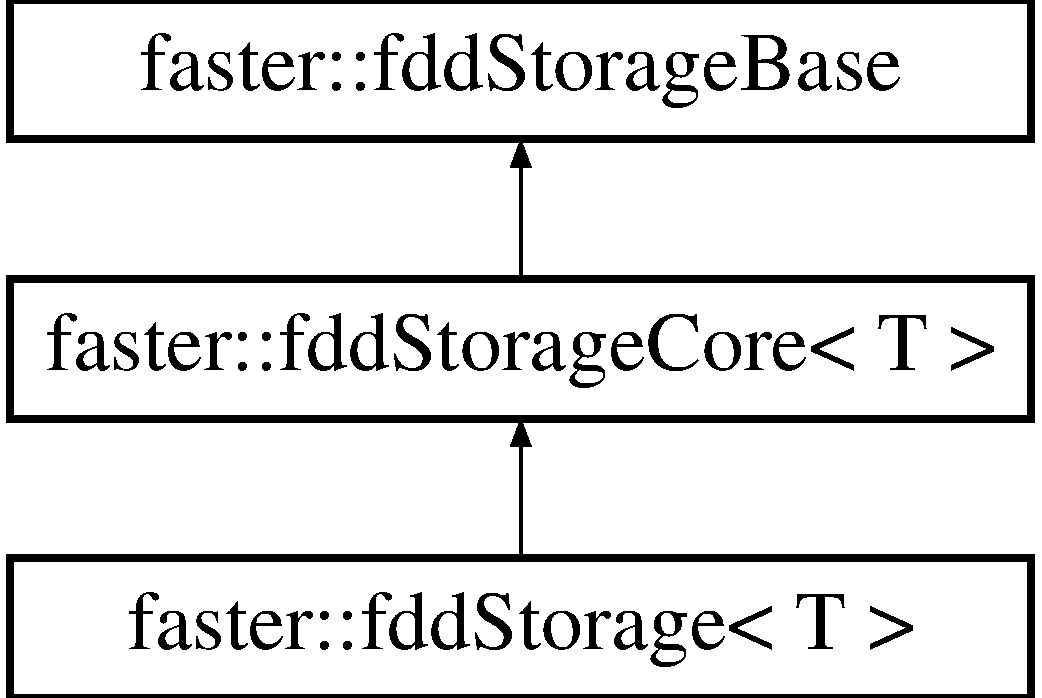
\includegraphics[height=3.000000cm]{classfaster_1_1fddStorageCore}
\end{center}
\end{figure}


\subsection{Description}
\subsubsection*{template$<$class T$>$\newline
class faster\+::fdd\+Storage\+Core$<$ T $>$}



Definition at line 13 of file fdd\+Storage.\+h.

\subsection*{Public Member Functions}
\begin{DoxyCompactItemize}
\item 
\hypertarget{classfaster_1_1fddStorageCore_aaae0b252366d73dec3995251fdc75920}{}\label{classfaster_1_1fddStorageCore_aaae0b252366d73dec3995251fdc75920} 
{\bfseries fdd\+Storage\+Core} (size\+\_\+t s)
\item 
\hypertarget{classfaster_1_1fddStorageCore_aa3d19bc27af39d838226ab3e196beb15}{}\label{classfaster_1_1fddStorageCore_aa3d19bc27af39d838226ab3e196beb15} 
T $\ast$ {\bfseries get\+Data} ()
\item 
\hypertarget{classfaster_1_1fddStorageCore_a6bf9e9e16bdcaf4164ac5a3d28848ec0}{}\label{classfaster_1_1fddStorageCore_a6bf9e9e16bdcaf4164ac5a3d28848ec0} 
void {\bfseries set\+Size} (size\+\_\+t s U\+N\+U\+S\+ED)
\item 
\hypertarget{classfaster_1_1fddStorageCore_ad4608901a31ab093edc8be2a3852a014}{}\label{classfaster_1_1fddStorageCore_ad4608901a31ab093edc8be2a3852a014} 
T \& {\bfseries operator\mbox{[}$\,$\mbox{]}} (size\+\_\+t ref)
\end{DoxyCompactItemize}
\subsection*{Protected Attributes}
\begin{DoxyCompactItemize}
\item 
\hypertarget{classfaster_1_1fddStorageCore_af2b22b0cda86b521472708991c38b797}{}\label{classfaster_1_1fddStorageCore_af2b22b0cda86b521472708991c38b797} 
T $\ast$ {\bfseries local\+Data}
\end{DoxyCompactItemize}


The documentation for this class was generated from the following files\+:\begin{DoxyCompactItemize}
\item 
/home/mtcs/pesquisa/faster/faster.\+git/src/include/fdd\+Storage.\+h\item 
/home/mtcs/pesquisa/faster/faster.\+git/src/libfaster/fdd\+Storage.\+cpp\end{DoxyCompactItemize}

\hypertarget{classfaster_1_1groupedFdd}{}\section{faster\+:\+:grouped\+Fdd$<$ K $>$ Class Template Reference}
\label{classfaster_1_1groupedFdd}\index{faster\+::grouped\+Fdd$<$ K $>$@{faster\+::grouped\+Fdd$<$ K $>$}}
Inheritance diagram for faster\+:\+:grouped\+Fdd$<$ K $>$\+:\begin{figure}[H]
\begin{center}
\leavevmode
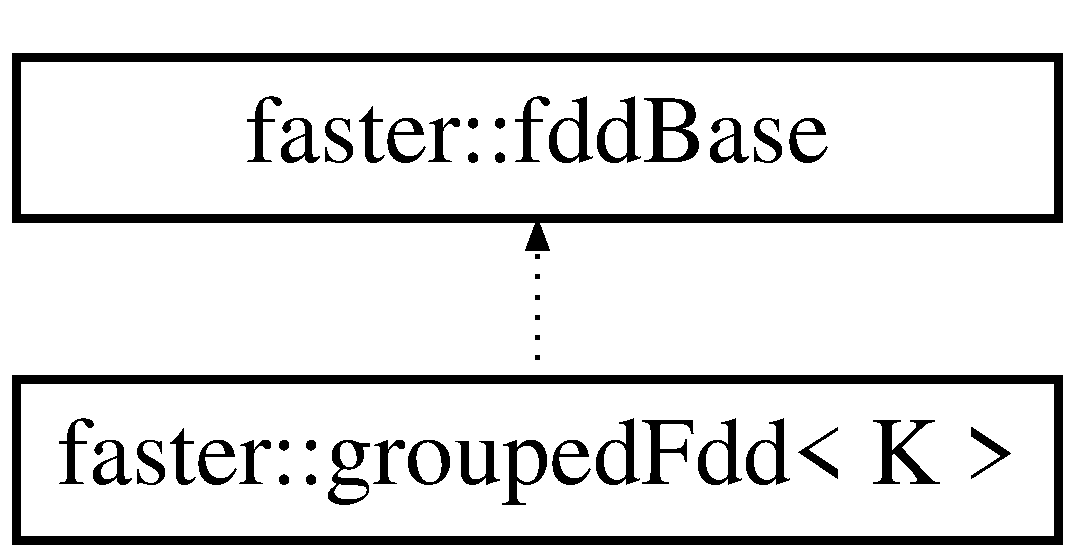
\includegraphics[height=2.000000cm]{classfaster_1_1groupedFdd}
\end{center}
\end{figure}


\subsection{Description}
\subsubsection*{template$<$typename K$>$\newline
class faster\+::grouped\+Fdd$<$ K $>$}



Definition at line 55 of file grouped\+Fdd.\+h.

\subsection*{Public Member Functions}
\begin{DoxyCompactItemize}
\item 
{\footnotesize template$<$typename T , typename U $>$ }\\\hyperlink{classfaster_1_1groupedFdd_a3e057f8351843ebf4b2875d3bb763ccb}{grouped\+Fdd} (\hyperlink{classfaster_1_1fastContext}{fast\+Context} $\ast$c, \hyperlink{classfaster_1_1iFddCore}{i\+Fdd\+Core}$<$ K, T $>$ $\ast$fdd0, \hyperlink{classfaster_1_1iFddCore}{i\+Fdd\+Core}$<$ K, U $>$ $\ast$fdd1, system\+\_\+clock\+::time\+\_\+point \&start)
\begin{DoxyCompactList}\small\item\em Creates a \hyperlink{classfaster_1_1indexedFdd}{indexed\+Fdd} group with two members. \end{DoxyCompactList}\item 
{\footnotesize template$<$typename T , typename U , typename V $>$ }\\\hyperlink{classfaster_1_1groupedFdd_a0f6bb764367d709b4837afcdf2cf0c30}{grouped\+Fdd} (\hyperlink{classfaster_1_1fastContext}{fast\+Context} $\ast$c, \hyperlink{classfaster_1_1iFddCore}{i\+Fdd\+Core}$<$ K, T $>$ $\ast$fdd0, \hyperlink{classfaster_1_1iFddCore}{i\+Fdd\+Core}$<$ K, U $>$ $\ast$fdd1, \hyperlink{classfaster_1_1iFddCore}{i\+Fdd\+Core}$<$ K, V $>$ $\ast$fdd2, system\+\_\+clock\+::time\+\_\+point \&start)
\begin{DoxyCompactList}\small\item\em Creates a \hyperlink{classfaster_1_1indexedFdd}{indexed\+Fdd} group with two members. \end{DoxyCompactList}\item 
\hyperlink{classfaster_1_1groupedFdd}{grouped\+Fdd}$<$ K $>$ $\ast$ \hyperlink{group__memmodel_gaf1256330323bf97826eaa01b0bb91bc1}{cache} ()
\begin{DoxyCompactList}\small\item\em Prevents automatic memory deallocation from hapenning. \end{DoxyCompactList}\item 
void \hyperlink{group__memmodel_gabfbee9b73e344e5fd6f44a209f6c1762}{discard} ()
\begin{DoxyCompactList}\small\item\em deallocates previously cached fdd \end{DoxyCompactList}\item 
\hypertarget{classfaster_1_1groupedFdd_ad1ed9e32f977574a9e0a12396e6578aa}{}\label{classfaster_1_1groupedFdd_ad1ed9e32f977574a9e0a12396e6578aa} 
bool {\bfseries is\+Grouped\+By\+Key} ()
\item 
\hypertarget{classfaster_1_1groupedFdd_a9228818350b8ff2fdbeba48f06d57e00}{}\label{classfaster_1_1groupedFdd_a9228818350b8ff2fdbeba48f06d57e00} 
void {\bfseries set\+Grouped\+By\+Key} (bool gbk U\+N\+U\+S\+ED)
\item 
\hyperlink{classfaster_1_1groupedFdd}{grouped\+Fdd}$<$ K $>$ $\ast$ {\bfseries update\+By\+Key} (update\+By\+Key\+G2\+FunctionP$<$ K $>$ funcP)
\item 
\hyperlink{classfaster_1_1groupedFdd}{grouped\+Fdd}$<$ K $>$ $\ast$ {\bfseries update\+By\+Key} (update\+By\+Key\+G3\+FunctionP$<$ K $>$ funcP)
\item 
\hyperlink{classfaster_1_1groupedFdd}{grouped\+Fdd}$<$ K $>$ $\ast$ {\bfseries bulk\+Update} (bulk\+Update\+G2\+FunctionP$<$ K $>$ funcP)
\item 
\hyperlink{classfaster_1_1groupedFdd}{grouped\+Fdd}$<$ K $>$ $\ast$ {\bfseries bulk\+Update} (bulk\+Update\+G3\+FunctionP$<$ K $>$ funcP)
\item 
{\footnotesize template$<$typename Ko , typename To $>$ }\\\hyperlink{classfaster_1_1indexedFdd}{indexed\+Fdd}$<$ Ko, To $>$ $\ast$ {\bfseries map\+By\+Key} (Imap\+By\+Key\+G2\+FunctionP$<$ K, Ko, To $>$ funcP)
\item 
{\footnotesize template$<$typename Ko , typename To $>$ }\\\hyperlink{classfaster_1_1indexedFdd}{indexed\+Fdd}$<$ Ko, To $>$ $\ast$ {\bfseries map\+By\+Key} (Imap\+By\+Key\+G3\+FunctionP$<$ K, Ko, To $>$ funcP)
\item 
{\footnotesize template$<$typename To $>$ }\\\hyperlink{classfaster_1_1fdd}{fdd}$<$ To $>$ $\ast$ {\bfseries map\+By\+Key} (map\+By\+Key\+G2\+FunctionP$<$ K, To $>$ funcP)
\item 
{\footnotesize template$<$typename To $>$ }\\\hyperlink{classfaster_1_1fdd}{fdd}$<$ To $>$ $\ast$ {\bfseries map\+By\+Key} (map\+By\+Key\+G3\+FunctionP$<$ K, To $>$ funcP)
\item 
{\footnotesize template$<$typename Ko , typename To $>$ }\\\hyperlink{classfaster_1_1indexedFdd}{indexed\+Fdd}$<$ Ko, To $>$ $\ast$ {\bfseries flat\+Map\+By\+Key} (Iflat\+Map\+By\+Key\+G2\+FunctionP$<$ K, Ko, To $>$ funcP)
\item 
{\footnotesize template$<$typename Ko , typename To $>$ }\\\hyperlink{classfaster_1_1indexedFdd}{indexed\+Fdd}$<$ Ko, To $>$ $\ast$ {\bfseries flat\+Map\+By\+Key} (Iflat\+Map\+By\+Key\+G3\+FunctionP$<$ K, Ko, To $>$ funcP)
\item 
{\footnotesize template$<$typename To $>$ }\\\hyperlink{classfaster_1_1fdd}{fdd}$<$ To $>$ $\ast$ {\bfseries flat\+Map\+By\+Key} (flat\+Map\+By\+Key\+G2\+FunctionP$<$ K, To $>$ funcP)
\item 
{\footnotesize template$<$typename To $>$ }\\\hyperlink{classfaster_1_1fdd}{fdd}$<$ To $>$ $\ast$ {\bfseries flat\+Map\+By\+Key} (flat\+Map\+By\+Key\+G3\+FunctionP$<$ K, To $>$ funcP)
\item 
{\footnotesize template$<$typename Ko , typename To $>$ }\\\hyperlink{classfaster_1_1indexedFdd}{indexed\+Fdd}$<$ Ko, To $>$ $\ast$ {\bfseries bulk\+Flat\+Map} (Ibulk\+Flat\+Map\+G2\+FunctionP$<$ K, Ko, To $>$ funcP)
\item 
{\footnotesize template$<$typename Ko , typename To $>$ }\\\hyperlink{classfaster_1_1indexedFdd}{indexed\+Fdd}$<$ Ko, To $>$ $\ast$ {\bfseries bulk\+Flat\+Map} (Ibulk\+Flat\+Map\+G3\+FunctionP$<$ K, Ko, To $>$ funcP)
\item 
{\footnotesize template$<$typename To $>$ }\\\hyperlink{classfaster_1_1fdd}{fdd}$<$ To $>$ $\ast$ {\bfseries bulk\+Flat\+Map} (bulk\+Flat\+Map\+G2\+FunctionP$<$ K, To $>$ funcP)
\item 
{\footnotesize template$<$typename To $>$ }\\\hyperlink{classfaster_1_1fdd}{fdd}$<$ To $>$ $\ast$ {\bfseries bulk\+Flat\+Map} (bulk\+Flat\+Map\+G3\+FunctionP$<$ K, To $>$ funcP)
\end{DoxyCompactItemize}


\subsection{Constructors and Destructors}
\hypertarget{classfaster_1_1groupedFdd_a3e057f8351843ebf4b2875d3bb763ccb}{}\label{classfaster_1_1groupedFdd_a3e057f8351843ebf4b2875d3bb763ccb} 
\index{faster\+::grouped\+Fdd@{faster\+::grouped\+Fdd}!grouped\+Fdd@{grouped\+Fdd}}
\index{grouped\+Fdd@{grouped\+Fdd}!faster\+::grouped\+Fdd@{faster\+::grouped\+Fdd}}
\subsubsection{\texorpdfstring{grouped\+Fdd()}{groupedFdd()}\hspace{0.1cm}{\footnotesize\ttfamily [1/2]}}
{\footnotesize\ttfamily template$<$typename K$>$ \\
template$<$typename T , typename U $>$ \\
\hyperlink{classfaster_1_1groupedFdd}{faster\+::grouped\+Fdd}$<$ K $>$\+::\hyperlink{classfaster_1_1groupedFdd}{grouped\+Fdd} (\begin{DoxyParamCaption}\item[{\hyperlink{classfaster_1_1fastContext}{fast\+Context} $\ast$}]{c,  }\item[{\hyperlink{classfaster_1_1iFddCore}{i\+Fdd\+Core}$<$ K, T $>$ $\ast$}]{fdd0,  }\item[{\hyperlink{classfaster_1_1iFddCore}{i\+Fdd\+Core}$<$ K, U $>$ $\ast$}]{fdd1,  }\item[{system\+\_\+clock\+::time\+\_\+point \&}]{start }\end{DoxyParamCaption})\hspace{0.3cm}{\ttfamily [inline]}}



Creates a \hyperlink{classfaster_1_1indexedFdd}{indexed\+Fdd} group with two members. 


\begin{DoxyTemplParams}{Template Parameters}
{\em T} & -\/ value type of the first dataset \\
\hline
{\em U} & -\/ value type of the second dataset \\
\hline
\end{DoxyTemplParams}

\begin{DoxyParams}{Parameters}
{\em c} & -\/ the context \\
\hline
{\em fdd0} & -\/ first dataset \\
\hline
{\em fdd1} & -\/ second dataset \\
\hline
{\em start} & -\/ start timestamp \\
\hline
\end{DoxyParams}


Definition at line 87 of file grouped\+Fdd.\+h.

\hypertarget{classfaster_1_1groupedFdd_a0f6bb764367d709b4837afcdf2cf0c30}{}\label{classfaster_1_1groupedFdd_a0f6bb764367d709b4837afcdf2cf0c30} 
\index{faster\+::grouped\+Fdd@{faster\+::grouped\+Fdd}!grouped\+Fdd@{grouped\+Fdd}}
\index{grouped\+Fdd@{grouped\+Fdd}!faster\+::grouped\+Fdd@{faster\+::grouped\+Fdd}}
\subsubsection{\texorpdfstring{grouped\+Fdd()}{groupedFdd()}\hspace{0.1cm}{\footnotesize\ttfamily [2/2]}}
{\footnotesize\ttfamily template$<$typename K$>$ \\
template$<$typename T , typename U , typename V $>$ \\
\hyperlink{classfaster_1_1groupedFdd}{faster\+::grouped\+Fdd}$<$ K $>$\+::\hyperlink{classfaster_1_1groupedFdd}{grouped\+Fdd} (\begin{DoxyParamCaption}\item[{\hyperlink{classfaster_1_1fastContext}{fast\+Context} $\ast$}]{c,  }\item[{\hyperlink{classfaster_1_1iFddCore}{i\+Fdd\+Core}$<$ K, T $>$ $\ast$}]{fdd0,  }\item[{\hyperlink{classfaster_1_1iFddCore}{i\+Fdd\+Core}$<$ K, U $>$ $\ast$}]{fdd1,  }\item[{\hyperlink{classfaster_1_1iFddCore}{i\+Fdd\+Core}$<$ K, V $>$ $\ast$}]{fdd2,  }\item[{system\+\_\+clock\+::time\+\_\+point \&}]{start }\end{DoxyParamCaption})\hspace{0.3cm}{\ttfamily [inline]}}



Creates a \hyperlink{classfaster_1_1indexedFdd}{indexed\+Fdd} group with two members. 


\begin{DoxyTemplParams}{Template Parameters}
{\em T} & -\/ value type of the first dataset \\
\hline
{\em U} & -\/ value type of the second dataset \\
\hline
{\em V} & -\/ value type of the third dataset \\
\hline
\end{DoxyTemplParams}

\begin{DoxyParams}{Parameters}
{\em c} & -\/ the context \\
\hline
{\em fdd0} & -\/ first dataset \\
\hline
{\em fdd1} & -\/ second dataset \\
\hline
{\em fdd2} & -\/ third dataset \\
\hline
{\em start} & -\/ start timestamp \\
\hline
\end{DoxyParams}


Definition at line 104 of file grouped\+Fdd.\+h.



The documentation for this class was generated from the following file\+:\begin{DoxyCompactItemize}
\item 
/home/mtcs/pesquisa/faster/faster.\+git/src/include/grouped\+Fdd.\+h\end{DoxyCompactItemize}

\hypertarget{classfaster_1_1iFddCore}{}\section{faster\+:\+:i\+Fdd\+Core$<$ K, T $>$ Class Template Reference}
\label{classfaster_1_1iFddCore}\index{faster\+::i\+Fdd\+Core$<$ K, T $>$@{faster\+::i\+Fdd\+Core$<$ K, T $>$}}
Inheritance diagram for faster\+:\+:i\+Fdd\+Core$<$ K, T $>$\+:\begin{figure}[H]
\begin{center}
\leavevmode
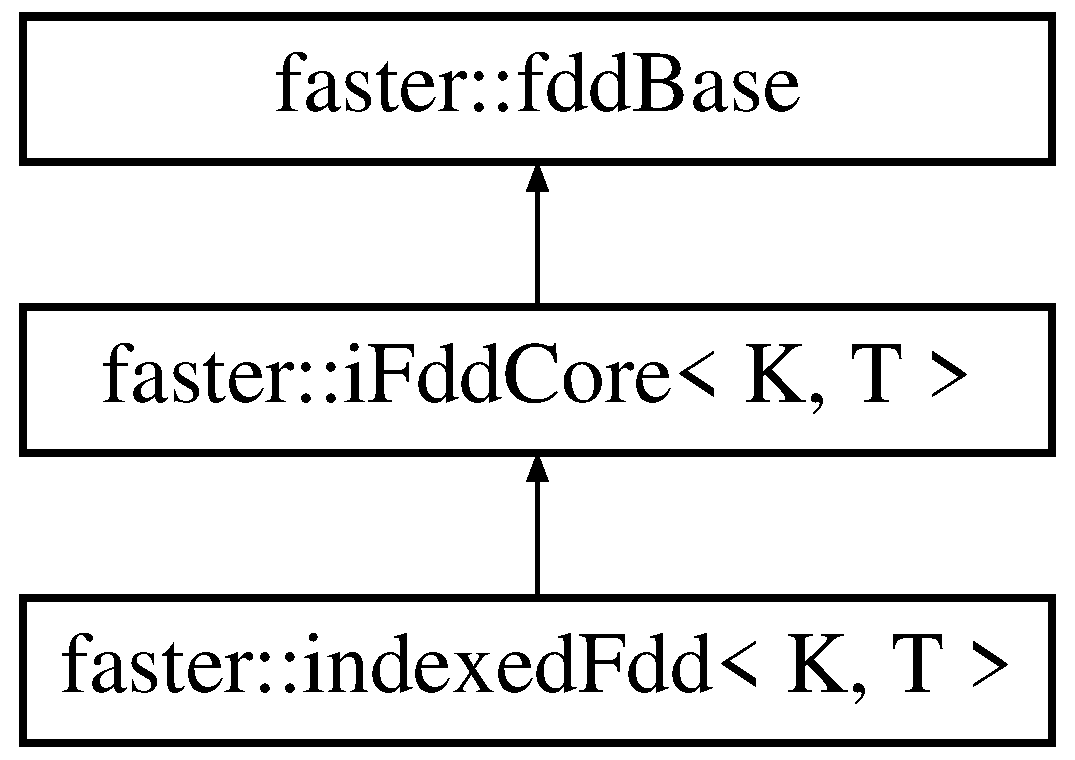
\includegraphics[height=3.000000cm]{classfaster_1_1iFddCore}
\end{center}
\end{figure}


\subsection{Description}
\subsubsection*{template$<$typename K, typename T$>$\newline
class faster\+::i\+Fdd\+Core$<$ K, T $>$}

\subsection*{Public Member Functions}
\begin{DoxyCompactItemize}
\item 
{\footnotesize template$<$typename U $>$ }\\\hyperlink{classfaster_1_1groupedFdd}{grouped\+Fdd}$<$ K $>$ $\ast$ \hyperlink{group__shuffle_ga311cd5a470392a25565057aaf0fa3226}{cogroup} (\hyperlink{classfaster_1_1iFddCore}{i\+Fdd\+Core}$<$ K, U $>$ $\ast$fdd1)
\begin{DoxyCompactList}\small\item\em Groupes two datasets twogether according with the keys of the first dataset. \end{DoxyCompactList}\item 
{\footnotesize template$<$typename U , typename V $>$ }\\\hyperlink{classfaster_1_1groupedFdd}{grouped\+Fdd}$<$ K $>$ $\ast$ \hyperlink{group__shuffle_gaf434c1c5118e380f9d78398fe46176d5}{cogroup} (\hyperlink{classfaster_1_1iFddCore}{i\+Fdd\+Core}$<$ K, U $>$ $\ast$fdd1, \hyperlink{classfaster_1_1iFddCore}{i\+Fdd\+Core}$<$ K, V $>$ $\ast$fdd2)
\begin{DoxyCompactList}\small\item\em Groupes tree datasets together according with the keys of the first dataset. \end{DoxyCompactList}\item 
std\+::unordered\+\_\+map$<$ K, size\+\_\+t $>$ \hyperlink{classfaster_1_1iFddCore_a4ed897a7b2af2918f91c3f8f89835ed4}{count\+By\+Key} ()
\begin{DoxyCompactList}\small\item\em Count how many unique key there is in the dataset. \end{DoxyCompactList}\item 
\hyperlink{classfaster_1_1indexedFdd}{indexed\+Fdd}$<$ K, T $>$ $\ast$ \hyperlink{group__shuffle_gac671d250f94c0927152362d4a982e931}{group\+By\+Key} ()
\begin{DoxyCompactList}\small\item\em Groups distributed dataset by key. \end{DoxyCompactList}\item 
void \hyperlink{group__memmodel_ga9a7002de9ec87e594aa461c1b379b453}{discard} ()
\begin{DoxyCompactList}\small\item\em deallocates previously cached F\+DD \end{DoxyCompactList}\item 
void \hyperlink{classfaster_1_1iFddCore_a6058211f45b0f603ff6e2ffab1976148}{write\+To\+File} (std\+::string path, std\+::string sufix)
\begin{DoxyCompactList}\small\item\em Writes F\+DD content to file. \end{DoxyCompactList}\item 
bool \hyperlink{classfaster_1_1iFddCore_a85b2607d1cc8f604a3965c313f16b240}{is\+Grouped\+By\+Key} ()
\begin{DoxyCompactList}\small\item\em Determines if a dataset is grouped by key. \end{DoxyCompactList}\item 
\hypertarget{classfaster_1_1iFddCore_a37c6f71cc6ce171ccd78120c7103f181}{}\label{classfaster_1_1iFddCore_a37c6f71cc6ce171ccd78120c7103f181} 
void \hyperlink{classfaster_1_1iFddCore_a37c6f71cc6ce171ccd78120c7103f181}{set\+Grouped\+By\+Key} (bool gbk)
\begin{DoxyCompactList}\small\item\em (U\+N\+U\+S\+ED) \end{DoxyCompactList}\item 
\hypertarget{classfaster_1_1iFddCore_a54fc3721d1e6291b9e741c7d5e2b7573}{}\label{classfaster_1_1iFddCore_a54fc3721d1e6291b9e741c7d5e2b7573} 
void \hyperlink{classfaster_1_1iFddCore_a54fc3721d1e6291b9e741c7d5e2b7573}{set\+Grouped\+By\+Map} (bool gbm)
\begin{DoxyCompactList}\small\item\em (U\+N\+U\+S\+ED) \end{DoxyCompactList}\end{DoxyCompactItemize}
\subsection*{Protected Member Functions}
\begin{DoxyCompactItemize}
\item 
\hypertarget{classfaster_1_1iFddCore_a5cdc2cf07bee57087e0997a0e140c9bd}{}\label{classfaster_1_1iFddCore_a5cdc2cf07bee57087e0997a0e140c9bd} 
{\bfseries i\+Fdd\+Core} (\hyperlink{classfaster_1_1fastContext}{fast\+Context} \&c)
\item 
\hypertarget{classfaster_1_1iFddCore_ab5be69b5752ab08168469e5baed451ef}{}\label{classfaster_1_1iFddCore_ab5be69b5752ab08168469e5baed451ef} 
{\bfseries i\+Fdd\+Core} (\hyperlink{classfaster_1_1fastContext}{fast\+Context} \&c, size\+\_\+t s, const std\+::vector$<$ size\+\_\+t $>$ \&data\+Alloc)
\item 
\hypertarget{classfaster_1_1iFddCore_a01a9a017ed4a89c3f7639452f242d364}{}\label{classfaster_1_1iFddCore_a01a9a017ed4a89c3f7639452f242d364} 
std\+::unordered\+\_\+map$<$ K, std\+::tuple$<$ size\+\_\+t, int, size\+\_\+t $>$ $>$ $\ast$ {\bfseries calculate\+Key\+Count} (std\+::vector$<$ std\+::pair$<$ void $\ast$, size\+\_\+t $>$ $>$ \&result)
\item 
\hypertarget{classfaster_1_1iFddCore_a9486ff6f13f33aa0d2e33d617eb75c99}{}\label{classfaster_1_1iFddCore_a9486ff6f13f33aa0d2e33d617eb75c99} 
std\+::unordered\+\_\+map$<$ K, int $>$ {\bfseries calculate\+Key\+Map} (std\+::unordered\+\_\+map$<$ K, std\+::tuple$<$ size\+\_\+t, int, size\+\_\+t $>$$>$ \&count)
\item 
\hypertarget{classfaster_1_1iFddCore_af5c3e4e57bf5931dbe861277e5035d42}{}\label{classfaster_1_1iFddCore_af5c3e4e57bf5931dbe861277e5035d42} 
void {\bfseries update} (void $\ast$funcP, \hyperlink{namespacefaster_a64379512d12d41c6e58f176939abfd80}{fdd\+Op\+Type} op)
\item 
\hypertarget{classfaster_1_1iFddCore_a483deae8e4c275dcbff0244ef33c2f4a}{}\label{classfaster_1_1iFddCore_a483deae8e4c275dcbff0244ef33c2f4a} 
\hyperlink{classfaster_1_1fddBase}{fdd\+Base} $\ast$ {\bfseries \+\_\+map} (void $\ast$funcP, \hyperlink{namespacefaster_a64379512d12d41c6e58f176939abfd80}{fdd\+Op\+Type} op, \hyperlink{classfaster_1_1fddBase}{fdd\+Base} $\ast$new\+Fdd, system\+\_\+clock\+::time\+\_\+point \&start)
\item 
\hypertarget{classfaster_1_1iFddCore_ad09cdfbaed755fb7c54b80d3bb6a4f63}{}\label{classfaster_1_1iFddCore_ad09cdfbaed755fb7c54b80d3bb6a4f63} 
{\footnotesize template$<$typename U $>$ }\\\hyperlink{classfaster_1_1fdd}{fdd}$<$ U $>$ $\ast$ {\bfseries map} (void $\ast$funcP, \hyperlink{namespacefaster_a64379512d12d41c6e58f176939abfd80}{fdd\+Op\+Type} op)
\item 
\hypertarget{classfaster_1_1iFddCore_a88bba48ad95225c4bceb986c13301212}{}\label{classfaster_1_1iFddCore_a88bba48ad95225c4bceb986c13301212} 
{\footnotesize template$<$typename L , typename U $>$ }\\\hyperlink{classfaster_1_1indexedFdd}{indexed\+Fdd}$<$ L, U $>$ $\ast$ {\bfseries mapI} (void $\ast$funcP, \hyperlink{namespacefaster_a64379512d12d41c6e58f176939abfd80}{fdd\+Op\+Type} op)
\item 
\hypertarget{classfaster_1_1iFddCore_a799f3c72257b159987443ad211dde11c}{}\label{classfaster_1_1iFddCore_a799f3c72257b159987443ad211dde11c} 
\hyperlink{classfaster_1_1indexedFdd}{indexed\+Fdd}$<$ K, T $>$ $\ast$ {\bfseries group\+By\+Key\+Mapped} ()
\item 
\hypertarget{classfaster_1_1iFddCore_acf8b2e5e6f2e45cf545b8738f89586ca}{}\label{classfaster_1_1iFddCore_acf8b2e5e6f2e45cf545b8738f89586ca} 
\hyperlink{classfaster_1_1indexedFdd}{indexed\+Fdd}$<$ K, T $>$ $\ast$ {\bfseries group\+By\+Key\+Hashed} ()
\end{DoxyCompactItemize}
\subsection*{Protected Attributes}
\begin{DoxyCompactItemize}
\item 
\hypertarget{classfaster_1_1iFddCore_a0fdbb128eb02349bcf1eedd637b70d7c}{}\label{classfaster_1_1iFddCore_a0fdbb128eb02349bcf1eedd637b70d7c} 
bool {\bfseries grouped\+By\+Key}
\item 
\hypertarget{classfaster_1_1iFddCore_a98b58a607883a33766dff4846342066c}{}\label{classfaster_1_1iFddCore_a98b58a607883a33766dff4846342066c} 
bool {\bfseries grouped\+By\+Map}
\item 
\hypertarget{classfaster_1_1iFddCore_a698ad6bbac1d23c82f83bac07cd49c02}{}\label{classfaster_1_1iFddCore_a698ad6bbac1d23c82f83bac07cd49c02} 
\hyperlink{classfaster_1_1fastContext}{fast\+Context} $\ast$ {\bfseries context}
\end{DoxyCompactItemize}


\subsection{Member Function Documentation}
\hypertarget{classfaster_1_1iFddCore_a4ed897a7b2af2918f91c3f8f89835ed4}{}\label{classfaster_1_1iFddCore_a4ed897a7b2af2918f91c3f8f89835ed4} 
\index{faster\+::i\+Fdd\+Core@{faster\+::i\+Fdd\+Core}!count\+By\+Key@{count\+By\+Key}}
\index{count\+By\+Key@{count\+By\+Key}!faster\+::i\+Fdd\+Core@{faster\+::i\+Fdd\+Core}}
\subsubsection{\texorpdfstring{count\+By\+Key()}{countByKey()}}
{\footnotesize\ttfamily template$<$typename K , typename T $>$ \\
std\+::unordered\+\_\+map$<$ K, size\+\_\+t $>$ \hyperlink{classfaster_1_1iFddCore}{faster\+::i\+Fdd\+Core}$<$ K, T $>$\+::count\+By\+Key (\begin{DoxyParamCaption}{ }\end{DoxyParamCaption})}



Count how many unique key there is in the dataset. 

\begin{DoxyReturn}{Returns}
a unordered\+\_\+map (hash) of the key count. 
\end{DoxyReturn}
\hypertarget{classfaster_1_1iFddCore_a85b2607d1cc8f604a3965c313f16b240}{}\label{classfaster_1_1iFddCore_a85b2607d1cc8f604a3965c313f16b240} 
\index{faster\+::i\+Fdd\+Core@{faster\+::i\+Fdd\+Core}!is\+Grouped\+By\+Key@{is\+Grouped\+By\+Key}}
\index{is\+Grouped\+By\+Key@{is\+Grouped\+By\+Key}!faster\+::i\+Fdd\+Core@{faster\+::i\+Fdd\+Core}}
\subsubsection{\texorpdfstring{is\+Grouped\+By\+Key()}{isGroupedByKey()}}
{\footnotesize\ttfamily template$<$typename K, typename T$>$ \\
bool \hyperlink{classfaster_1_1iFddCore}{faster\+::i\+Fdd\+Core}$<$ K, T $>$\+::is\+Grouped\+By\+Key (\begin{DoxyParamCaption}{ }\end{DoxyParamCaption})\hspace{0.3cm}{\ttfamily [inline]}, {\ttfamily [virtual]}}



Determines if a dataset is grouped by key. 

\begin{DoxyReturn}{Returns}
true is it has been groupe by key 
\end{DoxyReturn}


Implements \hyperlink{classfaster_1_1fddBase}{faster\+::fdd\+Base}.

\hypertarget{classfaster_1_1iFddCore_a6058211f45b0f603ff6e2ffab1976148}{}\label{classfaster_1_1iFddCore_a6058211f45b0f603ff6e2ffab1976148} 
\index{faster\+::i\+Fdd\+Core@{faster\+::i\+Fdd\+Core}!write\+To\+File@{write\+To\+File}}
\index{write\+To\+File@{write\+To\+File}!faster\+::i\+Fdd\+Core@{faster\+::i\+Fdd\+Core}}
\subsubsection{\texorpdfstring{write\+To\+File()}{writeToFile()}}
{\footnotesize\ttfamily template$<$typename K , typename T $>$ \\
void \hyperlink{classfaster_1_1iFddCore}{faster\+::i\+Fdd\+Core}$<$ K, T $>$\+::write\+To\+File (\begin{DoxyParamCaption}\item[{std\+::string}]{path,  }\item[{std\+::string}]{sufix }\end{DoxyParamCaption})}



Writes F\+DD content to file. 

Every process will write its own file with a rank number between the prefix and the suffix.


\begin{DoxyParams}{Parameters}
{\em path} & -\/ Prefix of the file path to be written \\
\hline
{\em sufix} & -\/ Sufix of the file path to be written \\
\hline
\end{DoxyParams}


The documentation for this class was generated from the following files\+:\begin{DoxyCompactItemize}
\item 
/home/mtcs/pesquisa/faster/faster.\+git/src/include/grouped\+Fdd.\+h\item 
/home/mtcs/pesquisa/faster/faster.\+git/src/include/indexed\+Fdd.\+h\end{DoxyCompactItemize}

\hypertarget{classfaster_1_1indexedFdd}{}\section{faster\+:\+:indexed\+Fdd$<$ K, T $>$ Class Template Reference}
\label{classfaster_1_1indexedFdd}\index{faster\+::indexed\+Fdd$<$ K, T $>$@{faster\+::indexed\+Fdd$<$ K, T $>$}}
Inheritance diagram for faster\+:\+:indexed\+Fdd$<$ K, T $>$\+:\begin{figure}[H]
\begin{center}
\leavevmode
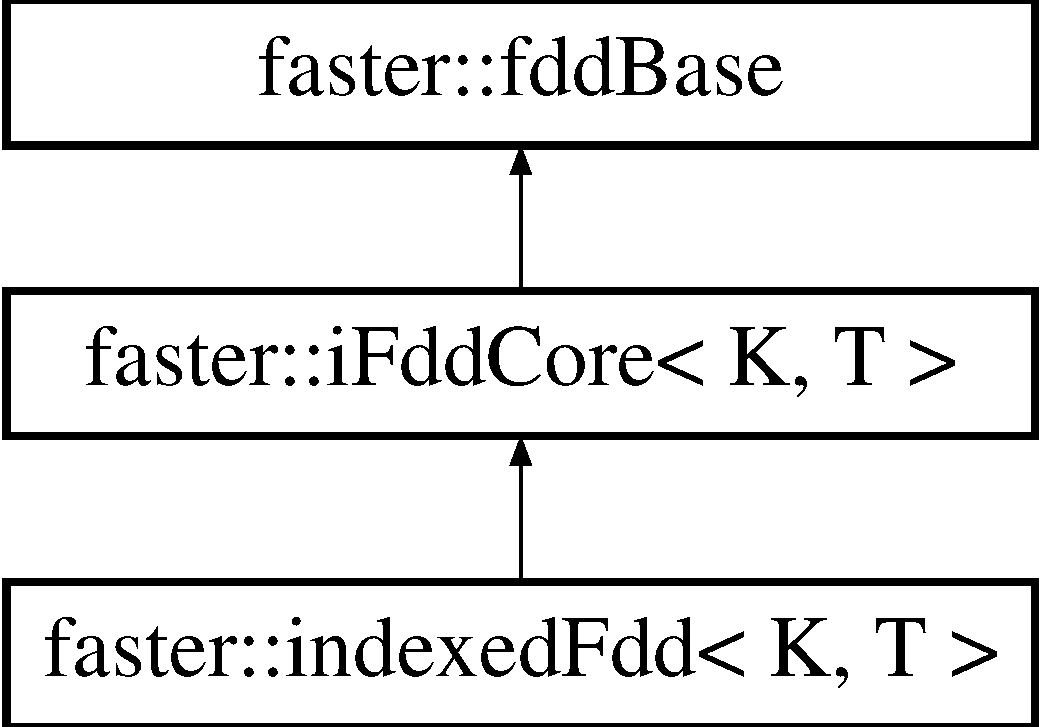
\includegraphics[height=3.000000cm]{classfaster_1_1indexedFdd}
\end{center}
\end{figure}


\subsection{Description}
\subsubsection*{template$<$typename K, typename T$>$\newline
class faster\+::indexed\+Fdd$<$ K, T $>$}



Definition at line 27 of file fast\+Context.\+h.

\subsection*{Public Member Functions}
\begin{DoxyCompactItemize}
\item 
\hypertarget{classfaster_1_1indexedFdd_a00f525684f5c451a2824e3244b256604}{}\label{classfaster_1_1indexedFdd_a00f525684f5c451a2824e3244b256604} 
\hyperlink{classfaster_1_1indexedFdd_a00f525684f5c451a2824e3244b256604}{indexed\+Fdd} (\hyperlink{classfaster_1_1fastContext}{fast\+Context} \&c)
\begin{DoxyCompactList}\small\item\em Create a empty \hyperlink{classfaster_1_1indexedFdd}{indexed\+Fdd}. \end{DoxyCompactList}\item 
\hypertarget{classfaster_1_1indexedFdd_abe773f041ad055a201b986bf5ed2903e}{}\label{classfaster_1_1indexedFdd_abe773f041ad055a201b986bf5ed2903e} 
\hyperlink{classfaster_1_1indexedFdd_abe773f041ad055a201b986bf5ed2903e}{indexed\+Fdd} (\hyperlink{classfaster_1_1fastContext}{fast\+Context} \&c, size\+\_\+t s, const std\+::vector$<$ size\+\_\+t $>$ \&data\+Alloc)
\begin{DoxyCompactList}\small\item\em Create a empty \hyperlink{classfaster_1_1indexedFdd}{indexed\+Fdd} with a pre allocated size. \end{DoxyCompactList}\item 
\hypertarget{classfaster_1_1indexedFdd_a9f6dc447c25e6bf1143348cbc2fff92d}{}\label{classfaster_1_1indexedFdd_a9f6dc447c25e6bf1143348cbc2fff92d} 
\hyperlink{classfaster_1_1indexedFdd_a9f6dc447c25e6bf1143348cbc2fff92d}{indexed\+Fdd} (\hyperlink{classfaster_1_1fastContext}{fast\+Context} \&c, size\+\_\+t s)
\begin{DoxyCompactList}\small\item\em Create a empty \hyperlink{classfaster_1_1indexedFdd}{indexed\+Fdd} with a pre allocated size. \end{DoxyCompactList}\item 
\hypertarget{classfaster_1_1indexedFdd_a2dcdec6b27dadc929564ff3023eba569}{}\label{classfaster_1_1indexedFdd_a2dcdec6b27dadc929564ff3023eba569} 
\hyperlink{classfaster_1_1indexedFdd_a2dcdec6b27dadc929564ff3023eba569}{indexed\+Fdd} (\hyperlink{classfaster_1_1fastContext}{fast\+Context} \&c, K $\ast$keys, T $\ast$data, size\+\_\+t size)
\begin{DoxyCompactList}\small\item\em Create a \hyperlink{classfaster_1_1indexedFdd}{indexed\+Fdd} from a array in memory. \end{DoxyCompactList}\item 
\hypertarget{classfaster_1_1indexedFdd_aab165b1eb0d4e7520187fdcca1505c37}{}\label{classfaster_1_1indexedFdd_aab165b1eb0d4e7520187fdcca1505c37} 
\hyperlink{classfaster_1_1indexedFdd_aab165b1eb0d4e7520187fdcca1505c37}{indexed\+Fdd} (\hyperlink{classfaster_1_1fastContext}{fast\+Context} \&c, std\+::string)
\begin{DoxyCompactList}\small\item\em Create a \hyperlink{classfaster_1_1indexedFdd}{indexed\+Fdd} from a file. \end{DoxyCompactList}\item 
\hypertarget{classfaster_1_1indexedFdd_a2ee1eb9ab82f8f6f825f374edf1af0f3}{}\label{classfaster_1_1indexedFdd_a2ee1eb9ab82f8f6f825f374edf1af0f3} 
\hyperlink{classfaster_1_1indexedFdd_a2ee1eb9ab82f8f6f825f374edf1af0f3}{$\sim$indexed\+Fdd} ()
\begin{DoxyCompactList}\small\item\em Class Destructor. W\+A\+R\+N\+I\+NG\+: It will deallocate distributed memory. \end{DoxyCompactList}\item 
std\+::vector$<$ std\+::pair$<$ K, T $>$ $>$ \hyperlink{classfaster_1_1indexedFdd_ae8222d15d17bb139bf07435227010607}{collect} ()
\begin{DoxyCompactList}\small\item\em Brings the distributted data from a indexed\+F\+DD to the driver memory. \end{DoxyCompactList}\item 
\hyperlink{classfaster_1_1indexedFdd}{indexed\+Fdd}$<$ K, T $>$ $\ast$ \hyperlink{group__memmodel_gadadcf78d4c0829655221ecdb29c952e2}{cache} ()
\begin{DoxyCompactList}\small\item\em Prevents automatic memory deallocation from hapenning. \end{DoxyCompactList}\item 
\hyperlink{classfaster_1_1indexedFdd}{indexed\+Fdd}$<$ K, T $>$ $\ast$ \hyperlink{group__update_gac1c08f691a992e6fdf17597d675a6bab}{update} (update\+I\+FunctionP$<$ K, T $>$ funcP)
\begin{DoxyCompactList}\small\item\em updates the content of a indexed\+F\+DD \end{DoxyCompactList}\item 
{\footnotesize template$<$typename L , typename U $>$ }\\\hyperlink{classfaster_1_1indexedFdd}{indexed\+Fdd}$<$ L, U $>$ $\ast$ \hyperlink{group__map_gae5d93ceaa1701aab3b3affc262ad3cc6}{map} (Imap\+I\+FunctionP$<$ K, T, L, U $>$ funcP)
\begin{DoxyCompactList}\small\item\em creates a indexed\+Fdd$<$\+L,\+U$>$ \end{DoxyCompactList}\item 
{\footnotesize template$<$typename L , typename U $>$ }\\\hyperlink{classfaster_1_1indexedFdd}{indexed\+Fdd}$<$ L, U $>$ $\ast$ \hyperlink{group__map_ga419f8dacfdbeb5f4d6d48e1c7a352fd8}{map} (I\+Pmap\+I\+FunctionP$<$ K, T, L, U $>$ funcP)
\begin{DoxyCompactList}\small\item\em creates a indexed\+Fdd$<$\+L,\+U$\ast$$>$ \end{DoxyCompactList}\item 
{\footnotesize template$<$typename U $>$ }\\\hyperlink{classfaster_1_1fdd}{fdd}$<$ U $>$ $\ast$ \hyperlink{group__map_ga9f6dad86bb02ecef29cf051609b50e37}{map} (map\+I\+FunctionP$<$ K, T, U $>$ funcP)
\begin{DoxyCompactList}\small\item\em creates a fdd$<$\+U$>$ \end{DoxyCompactList}\item 
{\footnotesize template$<$typename U $>$ }\\\hyperlink{classfaster_1_1fdd}{fdd}$<$ U $>$ $\ast$ \hyperlink{group__map_ga0c5c85eebcf016fdc39b7a52f1b965e1}{map} (Pmap\+I\+FunctionP$<$ K, T, U $>$ funcP)
\begin{DoxyCompactList}\small\item\em creates a fdd$<$\+U $\ast$$>$ \end{DoxyCompactList}\item 
{\footnotesize template$<$typename L , typename U $>$ }\\\hyperlink{classfaster_1_1indexedFdd}{indexed\+Fdd}$<$ L, U $>$ $\ast$ \hyperlink{group__bykey_ga72e66cd0a1896a9ba95e093ea665e5f9}{map\+By\+Key} (Imap\+By\+Key\+I\+FunctionP$<$ K, T, L, U $>$ funcP)
\begin{DoxyCompactList}\small\item\em creates a indexed\+Fdd$<$\+L,\+U$>$ \end{DoxyCompactList}\item 
{\footnotesize template$<$typename L , typename U $>$ }\\\hyperlink{classfaster_1_1indexedFdd}{indexed\+Fdd}$<$ L, U $>$ $\ast$ \hyperlink{group__bykey_gac1f7ce69086373cc5b419da1f8213bdd}{map\+By\+Key} (I\+Pmap\+By\+Key\+I\+FunctionP$<$ K, T, L, U $>$ funcP)
\begin{DoxyCompactList}\small\item\em creates a indexed\+Fdd$<$\+L,\+U$\ast$$>$ \end{DoxyCompactList}\item 
{\footnotesize template$<$typename L , typename U $>$ }\\\hyperlink{classfaster_1_1fdd}{fdd}$<$ U $>$ $\ast$ \hyperlink{group__bykey_ga993ec5033e2f665437f5d8590794fe0b}{map\+By\+Key} (map\+By\+Key\+I\+FunctionP$<$ K, T, U $>$ funcP)
\begin{DoxyCompactList}\small\item\em creates a fdd$<$\+U$>$ \end{DoxyCompactList}\item 
{\footnotesize template$<$typename L , typename U $>$ }\\\hyperlink{classfaster_1_1fdd}{fdd}$<$ U $>$ $\ast$ \hyperlink{group__bykey_ga558fd453f0a2ba00515359a46690972d}{map\+By\+Key} (Pmap\+By\+Key\+I\+FunctionP$<$ K, T, U $>$ funcP)
\begin{DoxyCompactList}\small\item\em creates a fdd$<$\+U $\ast$$>$ \end{DoxyCompactList}\item 
{\footnotesize template$<$typename L , typename U $>$ }\\\hyperlink{classfaster_1_1indexedFdd}{indexed\+Fdd}$<$ L, U $>$ $\ast$ \hyperlink{group__bulk_ga6ace49d5739205211ba154ada93c5a06}{bulk\+Map} (Ibulk\+Map\+I\+FunctionP$<$ K, T, L, U $>$ funcP)
\begin{DoxyCompactList}\small\item\em creates a indexed\+Fdd$<$\+L,\+U$>$ \end{DoxyCompactList}\item 
{\footnotesize template$<$typename L , typename U $>$ }\\\hyperlink{classfaster_1_1indexedFdd}{indexed\+Fdd}$<$ L, U $>$ $\ast$ \hyperlink{group__bulk_ga2989dde370e2c25e98434249a8cc5130}{bulk\+Map} (I\+Pbulk\+Map\+I\+FunctionP$<$ K, T, L, U $>$ funcP)
\begin{DoxyCompactList}\small\item\em creates a indexed\+Fdd$<$\+L,\+U$\ast$$>$ \end{DoxyCompactList}\item 
{\footnotesize template$<$typename L , typename U $>$ }\\\hyperlink{classfaster_1_1fdd}{fdd}$<$ U $>$ $\ast$ \hyperlink{group__bulk_ga661567a1e05b508619c9399b2149d7d7}{bulk\+Map} (bulk\+Map\+I\+FunctionP$<$ K, T, U $>$ funcP)
\begin{DoxyCompactList}\small\item\em creates a fdd$<$\+U$>$ \end{DoxyCompactList}\item 
{\footnotesize template$<$typename L , typename U $>$ }\\\hyperlink{classfaster_1_1fdd}{fdd}$<$ U $>$ $\ast$ \hyperlink{group__bulk_ga73ba7acbff0aabd4e8f92d07c3920d3a}{bulk\+Map} (Pbulk\+Map\+I\+FunctionP$<$ K, T, U $>$ funcP)
\begin{DoxyCompactList}\small\item\em creates a fdd$<$\+U $\ast$$>$ \end{DoxyCompactList}\item 
{\footnotesize template$<$typename L , typename U $>$ }\\\hyperlink{classfaster_1_1indexedFdd}{indexed\+Fdd}$<$ L, U $>$ $\ast$ \hyperlink{group__flatmap_ga9c104d832a84dc9f3f648db7c0ea1374}{flat\+Map} (Iflat\+Map\+I\+FunctionP$<$ K, T, L, U $>$ funcP)
\begin{DoxyCompactList}\small\item\em creates a indexed\+Fdd$<$\+L,\+U$>$ \end{DoxyCompactList}\item 
{\footnotesize template$<$typename L , typename U $>$ }\\\hyperlink{classfaster_1_1indexedFdd}{indexed\+Fdd}$<$ L, U $>$ $\ast$ \hyperlink{group__flatmap_gafe4a7200c3b0adfe13d9479b2e89d015}{flat\+Map} (I\+Pflat\+Map\+I\+FunctionP$<$ K, T, L, U $>$ funcP)
\begin{DoxyCompactList}\small\item\em creates a indexed\+Fdd$<$\+L,\+U$\ast$$>$ \end{DoxyCompactList}\item 
{\footnotesize template$<$typename L , typename U $>$ }\\\hyperlink{classfaster_1_1fdd}{fdd}$<$ U $>$ $\ast$ \hyperlink{group__flatmap_gac43ac811a8e6341d835990da6d43e422}{flat\+Map} (flat\+Map\+I\+FunctionP$<$ K, T, U $>$ funcP)
\begin{DoxyCompactList}\small\item\em creates a fdd$<$\+U$>$ \end{DoxyCompactList}\item 
{\footnotesize template$<$typename L , typename U $>$ }\\\hyperlink{classfaster_1_1fdd}{fdd}$<$ U $>$ $\ast$ \hyperlink{group__flatmap_gaa97f249971caca71c70a03bb170b3829}{flat\+Map} (Pflat\+Map\+I\+FunctionP$<$ K, T, U $>$ funcP)
\begin{DoxyCompactList}\small\item\em creates a fdd$<$\+U $\ast$$>$ \end{DoxyCompactList}\item 
{\footnotesize template$<$typename L , typename U $>$ }\\\hyperlink{classfaster_1_1indexedFdd}{indexed\+Fdd}$<$ L, U $>$ $\ast$ \hyperlink{group__bulk_ga3912bcd68abe5012c0573f1b2df4c5ad}{bulk\+Flat\+Map} (Ibulk\+Flat\+Map\+I\+FunctionP$<$ K, T, L, U $>$ funcP)
\begin{DoxyCompactList}\small\item\em creates a indexed\+Fdd$<$\+L,\+U$>$ \end{DoxyCompactList}\item 
{\footnotesize template$<$typename L , typename U $>$ }\\\hyperlink{classfaster_1_1indexedFdd}{indexed\+Fdd}$<$ L, U $>$ $\ast$ \hyperlink{group__bulk_ga1c49efc7eac095aaefb1446f31147536}{bulk\+Flat\+Map} (I\+Pbulk\+Flat\+Map\+I\+FunctionP$<$ K, T, L, U $>$ funcP)
\begin{DoxyCompactList}\small\item\em creates a indexed\+Fdd$<$\+L,\+U$\ast$$>$ \end{DoxyCompactList}\item 
{\footnotesize template$<$typename L , typename U $>$ }\\\hyperlink{classfaster_1_1fdd}{fdd}$<$ U $>$ $\ast$ \hyperlink{group__bulk_gaa06dfd667524b0ec9e10edf666414715}{bulk\+Flat\+Map} (bulk\+Flat\+Map\+I\+FunctionP$<$ K, T, U $>$ funcP)
\begin{DoxyCompactList}\small\item\em creates a fdd$<$\+U$>$ \end{DoxyCompactList}\item 
{\footnotesize template$<$typename L , typename U $>$ }\\\hyperlink{classfaster_1_1fdd}{fdd}$<$ U $>$ $\ast$ \hyperlink{group__bulk_ga811004fa92fc8685402fd10584b7863a}{bulk\+Flat\+Map} (Pbulk\+Flat\+Map\+I\+FunctionP$<$ K, T, U $>$ funcP)
\begin{DoxyCompactList}\small\item\em creates a fdd$<$\+U $\ast$$>$ \end{DoxyCompactList}\item 
std\+::pair$<$ K, T $>$ \hyperlink{group__flatmap_ga1b2c52816eb473decdd3e06c70db255b}{reduce} (Ireduce\+I\+FunctionP$<$ K, T $>$ funcP)
\begin{DoxyCompactList}\small\item\em summarizes a fdd$<$\+K,\+T$>$ into a single value of type T \end{DoxyCompactList}\item 
std\+::pair$<$ K, T $>$ \hyperlink{group__bulk_gac3086716ca3ee4490d76cfb23bce1f62}{bulk\+Reduce} (Ibulk\+Reduce\+I\+FunctionP$<$ K, T $>$ funcP)
\begin{DoxyCompactList}\small\item\em summarizes a fdd$<$\+K,\+T$>$ into a single value of type T using a bulk function {\itshape pair$<$\+K,\+T$>$ F(\+K, T, K, T)} \end{DoxyCompactList}\end{DoxyCompactItemize}
\subsection*{Additional Inherited Members}


\subsection{Member Function Documentation}
\hypertarget{classfaster_1_1indexedFdd_ae8222d15d17bb139bf07435227010607}{}\label{classfaster_1_1indexedFdd_ae8222d15d17bb139bf07435227010607} 
\index{faster\+::indexed\+Fdd@{faster\+::indexed\+Fdd}!collect@{collect}}
\index{collect@{collect}!faster\+::indexed\+Fdd@{faster\+::indexed\+Fdd}}
\subsubsection{\texorpdfstring{collect()}{collect()}}
{\footnotesize\ttfamily template$<$typename K, typename T$>$ \\
std\+::vector$<$std\+::pair$<$K,T$>$ $>$ \hyperlink{classfaster_1_1indexedFdd}{faster\+::indexed\+Fdd}$<$ K, T $>$\+::collect (\begin{DoxyParamCaption}{ }\end{DoxyParamCaption})\hspace{0.3cm}{\ttfamily [inline]}}



Brings the distributted data from a indexed\+F\+DD to the driver memory. 

\begin{DoxyReturn}{Returns}
a vector with the content of the indexed\+F\+DD 
\end{DoxyReturn}


Definition at line 211 of file indexed\+Fdd.\+h.



The documentation for this class was generated from the following files\+:\begin{DoxyCompactItemize}
\item 
/home/mtcs/pesquisa/faster/faster.\+git/src/include/fast\+Context.\+h\item 
/home/mtcs/pesquisa/faster/faster.\+git/src/include/indexed\+Fdd.\+h\end{DoxyCompactItemize}

\hypertarget{classfaster_1_1indexedFdd_3_01K_00_01T_01_5_01_4}{}\section{faster\+:\+:indexed\+Fdd$<$ K, T $\ast$ $>$ Class Template Reference}
\label{classfaster_1_1indexedFdd_3_01K_00_01T_01_5_01_4}\index{faster\+::indexed\+Fdd$<$ K, T $\ast$ $>$@{faster\+::indexed\+Fdd$<$ K, T $\ast$ $>$}}
Inheritance diagram for faster\+:\+:indexed\+Fdd$<$ K, T $\ast$ $>$\+:\begin{figure}[H]
\begin{center}
\leavevmode
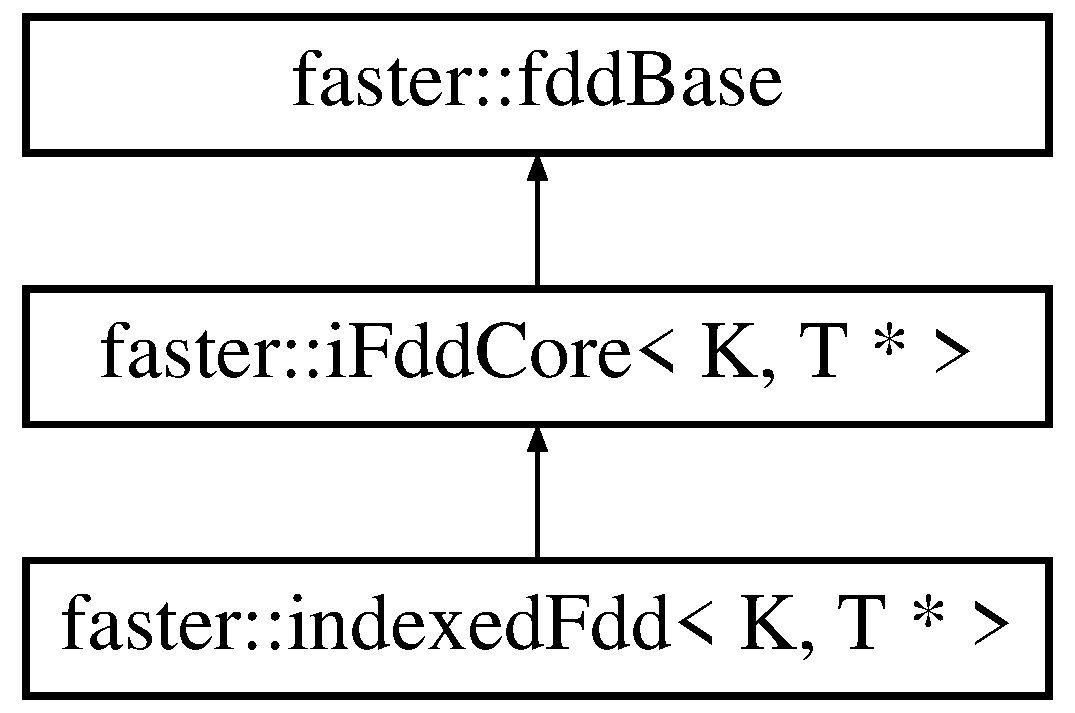
\includegraphics[height=3.000000cm]{classfaster_1_1indexedFdd_3_01K_00_01T_01_5_01_4}
\end{center}
\end{figure}


\subsection{Description}
\subsubsection*{template$<$typename K, typename T$>$\newline
class faster\+::indexed\+Fdd$<$ K, T $\ast$ $>$}

\subsection*{Public Member Functions}
\begin{DoxyCompactItemize}
\item 
\hypertarget{classfaster_1_1indexedFdd_3_01K_00_01T_01_5_01_4_a87aee6dcc77e70ba4447d8bbc763c407}{}\label{classfaster_1_1indexedFdd_3_01K_00_01T_01_5_01_4_a87aee6dcc77e70ba4447d8bbc763c407} 
{\bfseries indexed\+Fdd} (\hyperlink{classfaster_1_1fastContext}{fast\+Context} \&c)
\item 
\hypertarget{classfaster_1_1indexedFdd_3_01K_00_01T_01_5_01_4_aec3fecef4bfa9f08895ed89045e8462a}{}\label{classfaster_1_1indexedFdd_3_01K_00_01T_01_5_01_4_aec3fecef4bfa9f08895ed89045e8462a} 
{\bfseries indexed\+Fdd} (\hyperlink{classfaster_1_1fastContext}{fast\+Context} \&c, size\+\_\+t s, const std\+::vector$<$ size\+\_\+t $>$ \&data\+Alloc)
\item 
\hypertarget{classfaster_1_1indexedFdd_3_01K_00_01T_01_5_01_4_a36bc7e44015d4d79ed35dbbea6d6ff98}{}\label{classfaster_1_1indexedFdd_3_01K_00_01T_01_5_01_4_a36bc7e44015d4d79ed35dbbea6d6ff98} 
{\bfseries indexed\+Fdd} (\hyperlink{classfaster_1_1fastContext}{fast\+Context} \&c, size\+\_\+t s)
\item 
\hypertarget{classfaster_1_1indexedFdd_3_01K_00_01T_01_5_01_4_a4e9372f28592b79a12659db3c0f0d725}{}\label{classfaster_1_1indexedFdd_3_01K_00_01T_01_5_01_4_a4e9372f28592b79a12659db3c0f0d725} 
{\bfseries indexed\+Fdd} (\hyperlink{classfaster_1_1fastContext}{fast\+Context} \&c, K $\ast$keys, T $\ast$$\ast$data, size\+\_\+t $\ast$data\+Sizes, size\+\_\+t size)
\item 
\hypertarget{classfaster_1_1indexedFdd_3_01K_00_01T_01_5_01_4_ac415b9ac120e7f41daae599b04ed4e9d}{}\label{classfaster_1_1indexedFdd_3_01K_00_01T_01_5_01_4_ac415b9ac120e7f41daae599b04ed4e9d} 
{\footnotesize template$<$typename L , typename U $>$ }\\\hyperlink{classfaster_1_1indexedFdd}{indexed\+Fdd}$<$ L, U $>$ $\ast$ {\bfseries map} (Imap\+I\+P\+FunctionP$<$ K, T, L, U $>$ funcP)
\item 
\hypertarget{classfaster_1_1indexedFdd_3_01K_00_01T_01_5_01_4_a76632c9cc360bc0b0074a5d6d5a33fa9}{}\label{classfaster_1_1indexedFdd_3_01K_00_01T_01_5_01_4_a76632c9cc360bc0b0074a5d6d5a33fa9} 
{\footnotesize template$<$typename L , typename U $>$ }\\\hyperlink{classfaster_1_1indexedFdd}{indexed\+Fdd}$<$ L, U $>$ $\ast$ {\bfseries map} (I\+Pmap\+I\+P\+FunctionP$<$ K, T, L, U $>$ funcP)
\item 
\hypertarget{classfaster_1_1indexedFdd_3_01K_00_01T_01_5_01_4_a1feea9d9d94fa8dfec742d3c7a5c78f3}{}\label{classfaster_1_1indexedFdd_3_01K_00_01T_01_5_01_4_a1feea9d9d94fa8dfec742d3c7a5c78f3} 
{\footnotesize template$<$typename L , typename U $>$ }\\\hyperlink{classfaster_1_1fdd}{fdd}$<$ U $>$ $\ast$ {\bfseries map} (map\+I\+P\+FunctionP$<$ K, T, U $>$ funcP)
\item 
\hypertarget{classfaster_1_1indexedFdd_3_01K_00_01T_01_5_01_4_a24e59e4384848977c9b4210f83246955}{}\label{classfaster_1_1indexedFdd_3_01K_00_01T_01_5_01_4_a24e59e4384848977c9b4210f83246955} 
{\footnotesize template$<$typename L , typename U $>$ }\\\hyperlink{classfaster_1_1fdd}{fdd}$<$ U $>$ $\ast$ {\bfseries map} (Pmap\+I\+P\+FunctionP$<$ K, T, U $>$ funcP)
\item 
\hypertarget{classfaster_1_1indexedFdd_3_01K_00_01T_01_5_01_4_ae149988f4e281c18df0565cc315933ad}{}\label{classfaster_1_1indexedFdd_3_01K_00_01T_01_5_01_4_ae149988f4e281c18df0565cc315933ad} 
{\footnotesize template$<$typename L , typename U $>$ }\\\hyperlink{classfaster_1_1indexedFdd}{indexed\+Fdd}$<$ L, U $>$ $\ast$ {\bfseries map\+By\+Key} (Imap\+By\+Key\+I\+P\+FunctionP$<$ K, T, L, U $>$ funcP)
\item 
\hypertarget{classfaster_1_1indexedFdd_3_01K_00_01T_01_5_01_4_aaf721efd428dd2c7bbf748b8add0054e}{}\label{classfaster_1_1indexedFdd_3_01K_00_01T_01_5_01_4_aaf721efd428dd2c7bbf748b8add0054e} 
{\footnotesize template$<$typename L , typename U $>$ }\\\hyperlink{classfaster_1_1indexedFdd}{indexed\+Fdd}$<$ L, U $>$ $\ast$ {\bfseries map\+By\+Key} (I\+Pmap\+By\+Key\+I\+P\+FunctionP$<$ K, T, L, U $>$ funcP)
\item 
\hypertarget{classfaster_1_1indexedFdd_3_01K_00_01T_01_5_01_4_a0a02cf2c645ba2aa782ddba70c37e92c}{}\label{classfaster_1_1indexedFdd_3_01K_00_01T_01_5_01_4_a0a02cf2c645ba2aa782ddba70c37e92c} 
{\footnotesize template$<$typename L , typename U $>$ }\\\hyperlink{classfaster_1_1fdd}{fdd}$<$ U $>$ $\ast$ {\bfseries map\+By\+Key} (map\+By\+Key\+I\+P\+FunctionP$<$ K, T, U $>$ funcP)
\item 
\hypertarget{classfaster_1_1indexedFdd_3_01K_00_01T_01_5_01_4_a85e5688a87090e41f9a4d1b6c37f63c2}{}\label{classfaster_1_1indexedFdd_3_01K_00_01T_01_5_01_4_a85e5688a87090e41f9a4d1b6c37f63c2} 
{\footnotesize template$<$typename L , typename U $>$ }\\\hyperlink{classfaster_1_1fdd}{fdd}$<$ U $>$ $\ast$ {\bfseries map\+By\+Key} (Pmap\+By\+Key\+I\+P\+FunctionP$<$ K, T, U $>$ funcP)
\item 
\hypertarget{classfaster_1_1indexedFdd_3_01K_00_01T_01_5_01_4_a7a03d69db76df4ac10207baf44a13dd7}{}\label{classfaster_1_1indexedFdd_3_01K_00_01T_01_5_01_4_a7a03d69db76df4ac10207baf44a13dd7} 
{\footnotesize template$<$typename L , typename U $>$ }\\\hyperlink{classfaster_1_1indexedFdd}{indexed\+Fdd}$<$ L, U $>$ $\ast$ {\bfseries bulk\+Map} (Ibulk\+Map\+I\+P\+FunctionP$<$ K, T, L, U $>$ funcP)
\item 
\hypertarget{classfaster_1_1indexedFdd_3_01K_00_01T_01_5_01_4_a1544d5a014659d2993ff587ca96bcc9a}{}\label{classfaster_1_1indexedFdd_3_01K_00_01T_01_5_01_4_a1544d5a014659d2993ff587ca96bcc9a} 
{\footnotesize template$<$typename L , typename U $>$ }\\\hyperlink{classfaster_1_1indexedFdd}{indexed\+Fdd}$<$ L, U $>$ $\ast$ {\bfseries bulk\+Map} (I\+Pbulk\+Map\+I\+P\+FunctionP$<$ K, T, L, U $>$ funcP)
\item 
\hypertarget{classfaster_1_1indexedFdd_3_01K_00_01T_01_5_01_4_a148ae81fad5148a618eddb89fce2c349}{}\label{classfaster_1_1indexedFdd_3_01K_00_01T_01_5_01_4_a148ae81fad5148a618eddb89fce2c349} 
{\footnotesize template$<$typename L , typename U $>$ }\\\hyperlink{classfaster_1_1fdd}{fdd}$<$ U $>$ $\ast$ {\bfseries bulk\+Map} (bulk\+Map\+I\+P\+FunctionP$<$ K, T, U $>$ funcP)
\item 
\hypertarget{classfaster_1_1indexedFdd_3_01K_00_01T_01_5_01_4_ac2c2942ebc4c1d6d119cccd04d1b553e}{}\label{classfaster_1_1indexedFdd_3_01K_00_01T_01_5_01_4_ac2c2942ebc4c1d6d119cccd04d1b553e} 
{\footnotesize template$<$typename L , typename U $>$ }\\\hyperlink{classfaster_1_1fdd}{fdd}$<$ U $>$ $\ast$ {\bfseries bulk\+Map} (Pbulk\+Map\+I\+P\+FunctionP$<$ K, T, U $>$ funcP)
\item 
\hypertarget{classfaster_1_1indexedFdd_3_01K_00_01T_01_5_01_4_a703888ba7bbf207faa844d80fad701cc}{}\label{classfaster_1_1indexedFdd_3_01K_00_01T_01_5_01_4_a703888ba7bbf207faa844d80fad701cc} 
{\footnotesize template$<$typename L , typename U $>$ }\\\hyperlink{classfaster_1_1indexedFdd}{indexed\+Fdd}$<$ L, U $>$ $\ast$ {\bfseries flat\+Map} (Iflat\+Map\+I\+P\+FunctionP$<$ K, T, L, U $>$ funcP)
\item 
\hypertarget{classfaster_1_1indexedFdd_3_01K_00_01T_01_5_01_4_a2e623a58ad9cf4ffba57db62475e1d2f}{}\label{classfaster_1_1indexedFdd_3_01K_00_01T_01_5_01_4_a2e623a58ad9cf4ffba57db62475e1d2f} 
{\footnotesize template$<$typename L , typename U $>$ }\\\hyperlink{classfaster_1_1indexedFdd}{indexed\+Fdd}$<$ L, U $>$ $\ast$ {\bfseries flat\+Map} (I\+Pflat\+Map\+I\+P\+FunctionP$<$ K, T, L, U $>$ funcP)
\item 
\hypertarget{classfaster_1_1indexedFdd_3_01K_00_01T_01_5_01_4_a09c9506df40a80d2bcce454bc920596e}{}\label{classfaster_1_1indexedFdd_3_01K_00_01T_01_5_01_4_a09c9506df40a80d2bcce454bc920596e} 
{\footnotesize template$<$typename L , typename U $>$ }\\\hyperlink{classfaster_1_1fdd}{fdd}$<$ U $>$ $\ast$ {\bfseries flat\+Map} (flat\+Map\+I\+P\+FunctionP$<$ K, T, U $>$ funcP)
\item 
\hypertarget{classfaster_1_1indexedFdd_3_01K_00_01T_01_5_01_4_aa648f93a40fbbaf5243f1694312ea02f}{}\label{classfaster_1_1indexedFdd_3_01K_00_01T_01_5_01_4_aa648f93a40fbbaf5243f1694312ea02f} 
{\footnotesize template$<$typename L , typename U $>$ }\\\hyperlink{classfaster_1_1fdd}{fdd}$<$ U $>$ $\ast$ {\bfseries flat\+Map} (Pflat\+Map\+I\+P\+FunctionP$<$ K, T, U $>$ funcP)
\item 
\hypertarget{classfaster_1_1indexedFdd_3_01K_00_01T_01_5_01_4_af3376937665a44f002412304798e6309}{}\label{classfaster_1_1indexedFdd_3_01K_00_01T_01_5_01_4_af3376937665a44f002412304798e6309} 
{\footnotesize template$<$typename L , typename U $>$ }\\\hyperlink{classfaster_1_1indexedFdd}{indexed\+Fdd}$<$ L, U $>$ $\ast$ {\bfseries bulk\+Flat\+Map} (Ibulk\+Flat\+Map\+I\+P\+FunctionP$<$ K, T, L, U $>$ funcP)
\item 
\hypertarget{classfaster_1_1indexedFdd_3_01K_00_01T_01_5_01_4_ad584c7680b9f99bbdf7bc3f0fa91aeb4}{}\label{classfaster_1_1indexedFdd_3_01K_00_01T_01_5_01_4_ad584c7680b9f99bbdf7bc3f0fa91aeb4} 
{\footnotesize template$<$typename L , typename U $>$ }\\\hyperlink{classfaster_1_1indexedFdd}{indexed\+Fdd}$<$ L, U $>$ $\ast$ {\bfseries bulk\+Flat\+Map} (I\+Pbulk\+Flat\+Map\+I\+P\+FunctionP$<$ K, T, L, U $>$ funcP)
\item 
\hypertarget{classfaster_1_1indexedFdd_3_01K_00_01T_01_5_01_4_a1218ea8212678d867f9bcdb83a0374b9}{}\label{classfaster_1_1indexedFdd_3_01K_00_01T_01_5_01_4_a1218ea8212678d867f9bcdb83a0374b9} 
{\footnotesize template$<$typename L , typename U $>$ }\\\hyperlink{classfaster_1_1fdd}{fdd}$<$ U $>$ $\ast$ {\bfseries bulk\+Flat\+Map} (bulk\+Flat\+Map\+I\+P\+FunctionP$<$ K, T, U $>$ funcP)
\item 
\hypertarget{classfaster_1_1indexedFdd_3_01K_00_01T_01_5_01_4_a45def85f2fa284d9a8803c9c360cb8fb}{}\label{classfaster_1_1indexedFdd_3_01K_00_01T_01_5_01_4_a45def85f2fa284d9a8803c9c360cb8fb} 
{\footnotesize template$<$typename L , typename U $>$ }\\\hyperlink{classfaster_1_1fdd}{fdd}$<$ U $>$ $\ast$ {\bfseries bulk\+Flat\+Map} (Pbulk\+Flat\+Map\+I\+P\+FunctionP$<$ K, T, U $>$ funcP)
\item 
\hypertarget{classfaster_1_1indexedFdd_3_01K_00_01T_01_5_01_4_a39d927d2e023fc62647fad54b73f1c4b}{}\label{classfaster_1_1indexedFdd_3_01K_00_01T_01_5_01_4_a39d927d2e023fc62647fad54b73f1c4b} 
std\+::vector$<$ std\+::pair$<$ K, T $>$ $>$ {\bfseries reduce} (I\+Preduce\+I\+P\+FunctionP$<$ K, T $>$ funcP)
\item 
\hypertarget{classfaster_1_1indexedFdd_3_01K_00_01T_01_5_01_4_a0f89674fe2c844c623198bbdba8d58eb}{}\label{classfaster_1_1indexedFdd_3_01K_00_01T_01_5_01_4_a0f89674fe2c844c623198bbdba8d58eb} 
std\+::vector$<$ std\+::pair$<$ K, T $>$ $>$ {\bfseries bulk\+Reduce} (I\+Pbulk\+Reduce\+I\+P\+FunctionP$<$ K, T $>$ funcP)
\item 
\hypertarget{classfaster_1_1indexedFdd_3_01K_00_01T_01_5_01_4_a062614e61759dd430e27026e70280ac0}{}\label{classfaster_1_1indexedFdd_3_01K_00_01T_01_5_01_4_a062614e61759dd430e27026e70280ac0} 
std\+::vector$<$ std\+::tuple$<$ K, T $\ast$, size\+\_\+t $>$ $>$ {\bfseries collect} ()
\item 
\hypertarget{classfaster_1_1indexedFdd_3_01K_00_01T_01_5_01_4_a0285162c1cd6bb853daad827dd1f94fc}{}\label{classfaster_1_1indexedFdd_3_01K_00_01T_01_5_01_4_a0285162c1cd6bb853daad827dd1f94fc} 
\hyperlink{classfaster_1_1indexedFdd}{indexed\+Fdd}$<$ K, T $\ast$ $>$ $\ast$ {\bfseries cache} ()
\end{DoxyCompactItemize}
\subsection*{Additional Inherited Members}


The documentation for this class was generated from the following file\+:\begin{DoxyCompactItemize}
\item 
/home/mtcs/pesquisa/faster/faster.\+git/src/include/indexed\+Fdd.\+h\end{DoxyCompactItemize}

\hypertarget{classfaster_1_1indexedFddStorage}{}\section{faster\+:\+:indexed\+Fdd\+Storage$<$ K, T $>$ Class Template Reference}
\label{classfaster_1_1indexedFddStorage}\index{faster\+::indexed\+Fdd\+Storage$<$ K, T $>$@{faster\+::indexed\+Fdd\+Storage$<$ K, T $>$}}
Inheritance diagram for faster\+:\+:indexed\+Fdd\+Storage$<$ K, T $>$\+:\begin{figure}[H]
\begin{center}
\leavevmode
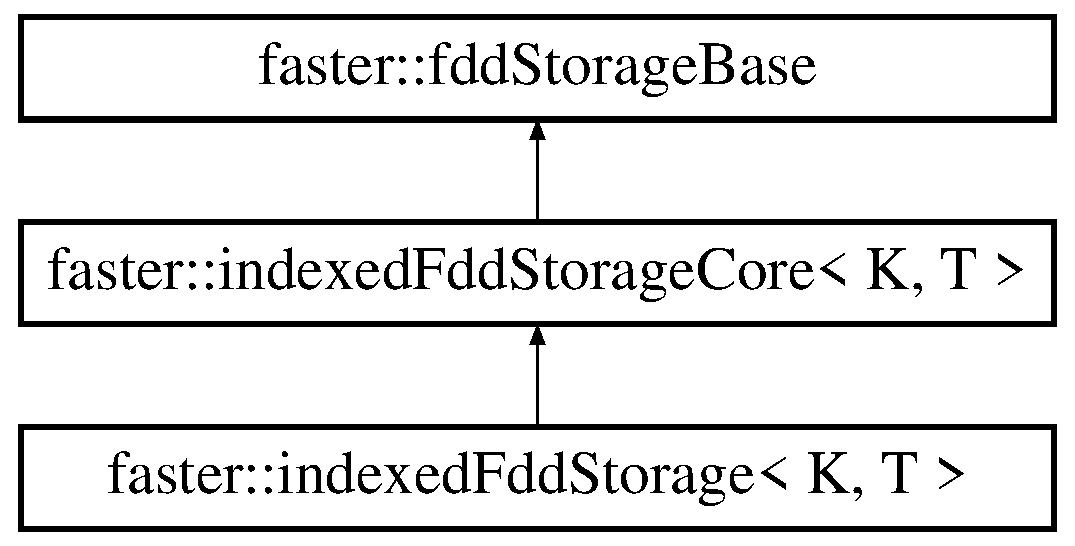
\includegraphics[height=3.000000cm]{classfaster_1_1indexedFddStorage}
\end{center}
\end{figure}


\subsection{Description}
\subsubsection*{template$<$class K, class T$>$\newline
class faster\+::indexed\+Fdd\+Storage$<$ K, T $>$}



Definition at line 23 of file \+\_\+worker\+I\+Fdd.\+h.

\subsection*{Public Member Functions}
\begin{DoxyCompactItemize}
\item 
\hypertarget{classfaster_1_1indexedFddStorage_ae23d28156db0adaf7ce85d59f3de83b8}{}\label{classfaster_1_1indexedFddStorage_ae23d28156db0adaf7ce85d59f3de83b8} 
{\bfseries indexed\+Fdd\+Storage} (size\+\_\+t s)
\item 
\hypertarget{classfaster_1_1indexedFddStorage_a0d632c3336dc752458bb9262c67f4c9a}{}\label{classfaster_1_1indexedFddStorage_a0d632c3336dc752458bb9262c67f4c9a} 
{\bfseries indexed\+Fdd\+Storage} (K $\ast$keys, T $\ast$data, size\+\_\+t s)
\item 
\hypertarget{classfaster_1_1indexedFddStorage_ae7c5b6ad85c386d8cffd904cb572d488}{}\label{classfaster_1_1indexedFddStorage_ae7c5b6ad85c386d8cffd904cb572d488} 
void {\bfseries set\+Data} (K $\ast$keys, T $\ast$data, size\+\_\+t s)
\item 
\hypertarget{classfaster_1_1indexedFddStorage_a9da343629ac1b2c725e4683177a3278b}{}\label{classfaster_1_1indexedFddStorage_a9da343629ac1b2c725e4683177a3278b} 
void {\bfseries set\+Data\+Raw} (void $\ast$keys, void $\ast$data, size\+\_\+t s)
\item 
\hypertarget{classfaster_1_1indexedFddStorage_a80f2ff6bb9c7b5a5cc04f22e4395596d}{}\label{classfaster_1_1indexedFddStorage_a80f2ff6bb9c7b5a5cc04f22e4395596d} 
void {\bfseries set\+Size} (size\+\_\+t s) override
\item 
\hypertarget{classfaster_1_1indexedFddStorage_a0a9fc58cdf64a108b43c1e4ec2d3a557}{}\label{classfaster_1_1indexedFddStorage_a0a9fc58cdf64a108b43c1e4ec2d3a557} 
void {\bfseries insert} (K key, T \&item)
\item 
\hypertarget{classfaster_1_1indexedFddStorage_a4e5ac4c4f6d1e32f5949361a54a29453}{}\label{classfaster_1_1indexedFddStorage_a4e5ac4c4f6d1e32f5949361a54a29453} 
void {\bfseries insert\+Raw} (void $\ast$d, size\+\_\+t s)
\item 
\hypertarget{classfaster_1_1indexedFddStorage_ad4430e7b86d905f3df6a10ee72d9de3d}{}\label{classfaster_1_1indexedFddStorage_ad4430e7b86d905f3df6a10ee72d9de3d} 
void {\bfseries grow} (size\+\_\+t to\+Size)
\item 
\hypertarget{classfaster_1_1indexedFddStorage_a8c235374da0dc7291a062abf2dd0b390}{}\label{classfaster_1_1indexedFddStorage_a8c235374da0dc7291a062abf2dd0b390} 
void {\bfseries shrink} ()
\end{DoxyCompactItemize}
\subsection*{Additional Inherited Members}


The documentation for this class was generated from the following files\+:\begin{DoxyCompactItemize}
\item 
/home/mtcs/pesquisa/faster/faster.\+git/src/include/\+\_\+worker\+I\+Fdd.\+h\item 
/home/mtcs/pesquisa/faster/faster.\+git/src/include/indexed\+Fdd\+Storage.\+h\item 
/home/mtcs/pesquisa/faster/faster.\+git/src/libfaster/indexed\+Fdd\+Storage.\+cpp\end{DoxyCompactItemize}

\hypertarget{classfaster_1_1indexedFddStorage_3_01K_00_01T_01_5_01_4}{}\section{faster\+:\+:indexed\+Fdd\+Storage$<$ K, T $\ast$ $>$ Class Template Reference}
\label{classfaster_1_1indexedFddStorage_3_01K_00_01T_01_5_01_4}\index{faster\+::indexed\+Fdd\+Storage$<$ K, T $\ast$ $>$@{faster\+::indexed\+Fdd\+Storage$<$ K, T $\ast$ $>$}}
Inheritance diagram for faster\+:\+:indexed\+Fdd\+Storage$<$ K, T $\ast$ $>$\+:\begin{figure}[H]
\begin{center}
\leavevmode
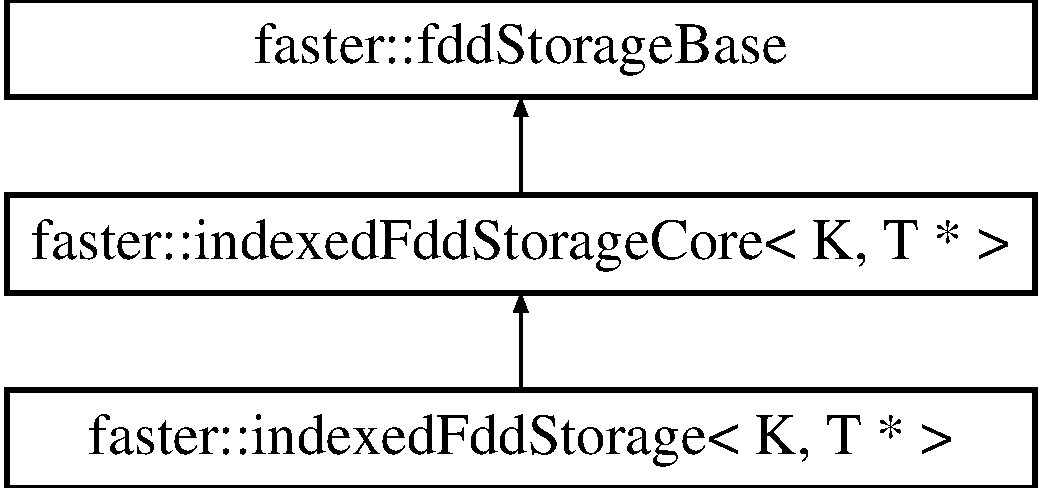
\includegraphics[height=3.000000cm]{classfaster_1_1indexedFddStorage_3_01K_00_01T_01_5_01_4}
\end{center}
\end{figure}
\subsection*{Public Member Functions}
\begin{DoxyCompactItemize}
\item 
\hypertarget{classfaster_1_1indexedFddStorage_3_01K_00_01T_01_5_01_4_a0ad6ad05d9ccd4601ce2718827e295c1}{}{\bfseries indexed\+Fdd\+Storage} (size\+\_\+t s)\label{classfaster_1_1indexedFddStorage_3_01K_00_01T_01_5_01_4_a0ad6ad05d9ccd4601ce2718827e295c1}

\item 
\hypertarget{classfaster_1_1indexedFddStorage_3_01K_00_01T_01_5_01_4_a95c98e657a0443c3d384d897a4f8cb35}{}{\bfseries indexed\+Fdd\+Storage} (K $\ast$keys, T $\ast$$\ast$data, size\+\_\+t $\ast$line\+Sizes, size\+\_\+t s)\label{classfaster_1_1indexedFddStorage_3_01K_00_01T_01_5_01_4_a95c98e657a0443c3d384d897a4f8cb35}

\item 
\hypertarget{classfaster_1_1indexedFddStorage_3_01K_00_01T_01_5_01_4_a1f25a359fc75622309cb7f181d8545ef}{}void {\bfseries set\+Data} (K $\ast$keys, T $\ast$$\ast$data, size\+\_\+t $\ast$line\+Sizes, size\+\_\+t s)\label{classfaster_1_1indexedFddStorage_3_01K_00_01T_01_5_01_4_a1f25a359fc75622309cb7f181d8545ef}

\item 
\hypertarget{classfaster_1_1indexedFddStorage_3_01K_00_01T_01_5_01_4_a20ede574def362eae00630166dd6ca10}{}void {\bfseries set\+Data\+Raw} (void $\ast$keys, void $\ast$data, size\+\_\+t $\ast$line\+Sizes, size\+\_\+t s)\label{classfaster_1_1indexedFddStorage_3_01K_00_01T_01_5_01_4_a20ede574def362eae00630166dd6ca10}

\item 
\hypertarget{classfaster_1_1indexedFddStorage_3_01K_00_01T_01_5_01_4_ab26b5b1dc0eea07fb002f7144defcaa5}{}void {\bfseries set\+Size} (size\+\_\+t s) override\label{classfaster_1_1indexedFddStorage_3_01K_00_01T_01_5_01_4_ab26b5b1dc0eea07fb002f7144defcaa5}

\item 
\hypertarget{classfaster_1_1indexedFddStorage_3_01K_00_01T_01_5_01_4_a2bff285398ff9e7eb830b2a966643679}{}void {\bfseries insert} (K key, T $\ast$\&item, size\+\_\+t s)\label{classfaster_1_1indexedFddStorage_3_01K_00_01T_01_5_01_4_a2bff285398ff9e7eb830b2a966643679}

\item 
\hypertarget{classfaster_1_1indexedFddStorage_3_01K_00_01T_01_5_01_4_aeedf936a68804ea1f9e0b287ec786a74}{}void {\bfseries insert\+Raw} (void $\ast$d, size\+\_\+t s)\label{classfaster_1_1indexedFddStorage_3_01K_00_01T_01_5_01_4_aeedf936a68804ea1f9e0b287ec786a74}

\item 
\hypertarget{classfaster_1_1indexedFddStorage_3_01K_00_01T_01_5_01_4_a43dbd5e349f514d6fc6875bc400d3061}{}size\+\_\+t $\ast$ {\bfseries get\+Line\+Sizes} ()\label{classfaster_1_1indexedFddStorage_3_01K_00_01T_01_5_01_4_a43dbd5e349f514d6fc6875bc400d3061}

\item 
\hypertarget{classfaster_1_1indexedFddStorage_3_01K_00_01T_01_5_01_4_a47a8f1370e5b9c5a5cff40e77b241731}{}void {\bfseries grow} (size\+\_\+t to\+Size)\label{classfaster_1_1indexedFddStorage_3_01K_00_01T_01_5_01_4_a47a8f1370e5b9c5a5cff40e77b241731}

\item 
\hypertarget{classfaster_1_1indexedFddStorage_3_01K_00_01T_01_5_01_4_a69e570aeb85d7e3f8e3d2878773e9567}{}void {\bfseries shrink} ()\label{classfaster_1_1indexedFddStorage_3_01K_00_01T_01_5_01_4_a69e570aeb85d7e3f8e3d2878773e9567}

\end{DoxyCompactItemize}
\subsection*{Additional Inherited Members}


The documentation for this class was generated from the following file\+:\begin{DoxyCompactItemize}
\item 
/home/mtcs/pesquisa/faster/faster.\+git/src/include/indexed\+Fdd\+Storage.\+h\end{DoxyCompactItemize}

\hypertarget{classfaster_1_1indexedFddStorageCore}{}\section{faster\+:\+:indexed\+Fdd\+Storage\+Core$<$ K, T $>$ Class Template Reference}
\label{classfaster_1_1indexedFddStorageCore}\index{faster\+::indexed\+Fdd\+Storage\+Core$<$ K, T $>$@{faster\+::indexed\+Fdd\+Storage\+Core$<$ K, T $>$}}
Inheritance diagram for faster\+:\+:indexed\+Fdd\+Storage\+Core$<$ K, T $>$\+:\begin{figure}[H]
\begin{center}
\leavevmode
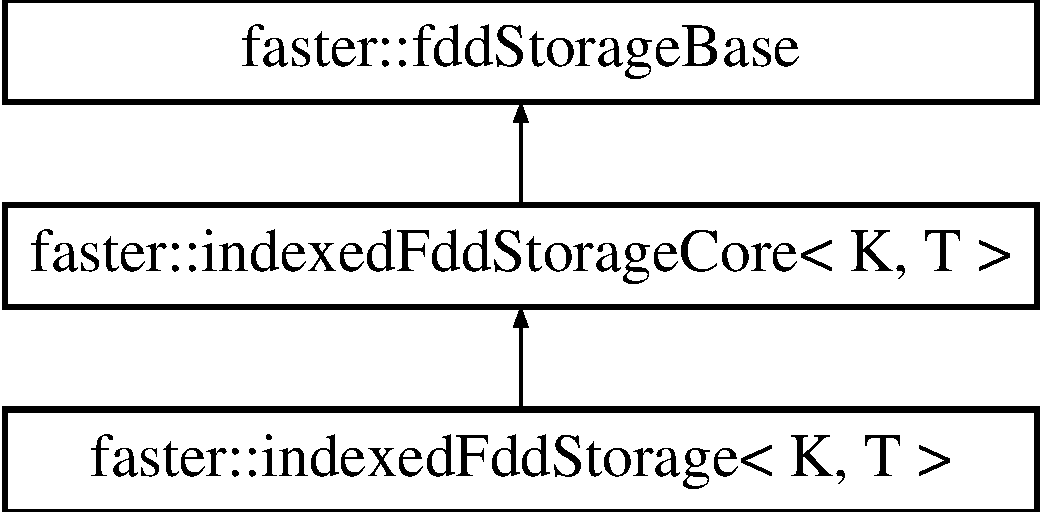
\includegraphics[height=3.000000cm]{classfaster_1_1indexedFddStorageCore}
\end{center}
\end{figure}


\subsection{Description}
\subsubsection*{template$<$class K, class T$>$\newline
class faster\+::indexed\+Fdd\+Storage\+Core$<$ K, T $>$}



Definition at line 15 of file indexed\+Fdd\+Storage.\+h.

\subsection*{Public Member Functions}
\begin{DoxyCompactItemize}
\item 
\hypertarget{classfaster_1_1indexedFddStorageCore_a8ef8f11997d28af03b02f84a632beeea}{}\label{classfaster_1_1indexedFddStorageCore_a8ef8f11997d28af03b02f84a632beeea} 
{\bfseries indexed\+Fdd\+Storage\+Core} (size\+\_\+t s)
\item 
\hypertarget{classfaster_1_1indexedFddStorageCore_ace53399ba953aa365a2121cadc613d77}{}\label{classfaster_1_1indexedFddStorageCore_ace53399ba953aa365a2121cadc613d77} 
T $\ast$ {\bfseries get\+Data} ()
\item 
\hypertarget{classfaster_1_1indexedFddStorageCore_a8c81c09139ac2042b0d15728317dc12b}{}\label{classfaster_1_1indexedFddStorageCore_a8c81c09139ac2042b0d15728317dc12b} 
K $\ast$ {\bfseries get\+Keys} ()
\item 
\hypertarget{classfaster_1_1indexedFddStorageCore_a8f39ec402c0c3307ae3df58e1a172743}{}\label{classfaster_1_1indexedFddStorageCore_a8f39ec402c0c3307ae3df58e1a172743} 
void {\bfseries set\+Size} (size\+\_\+t s U\+N\+U\+S\+ED)
\item 
\hypertarget{classfaster_1_1indexedFddStorageCore_a24cb4a85df359d86a39522a4f6ff7790}{}\label{classfaster_1_1indexedFddStorageCore_a24cb4a85df359d86a39522a4f6ff7790} 
T \& {\bfseries operator\mbox{[}$\,$\mbox{]}} (size\+\_\+t ref)
\item 
\hypertarget{classfaster_1_1indexedFddStorageCore_a36e8a7c036dad67bde3e34925b65f68d}{}\label{classfaster_1_1indexedFddStorageCore_a36e8a7c036dad67bde3e34925b65f68d} 
void {\bfseries sort\+By\+Key} ()
\end{DoxyCompactItemize}
\subsection*{Protected Attributes}
\begin{DoxyCompactItemize}
\item 
\hypertarget{classfaster_1_1indexedFddStorageCore_afc155f998bfe42973147af89bf75cfa5}{}\label{classfaster_1_1indexedFddStorageCore_afc155f998bfe42973147af89bf75cfa5} 
T $\ast$ {\bfseries local\+Data}
\item 
\hypertarget{classfaster_1_1indexedFddStorageCore_a4a31c9b81ef61a2aca489bdc010566f9}{}\label{classfaster_1_1indexedFddStorageCore_a4a31c9b81ef61a2aca489bdc010566f9} 
K $\ast$ {\bfseries local\+Keys}
\end{DoxyCompactItemize}


The documentation for this class was generated from the following files\+:\begin{DoxyCompactItemize}
\item 
/home/mtcs/pesquisa/faster/faster.\+git/src/include/indexed\+Fdd\+Storage.\+h\item 
/home/mtcs/pesquisa/faster/faster.\+git/src/libfaster/indexed\+Fdd\+Storage.\+cpp\end{DoxyCompactItemize}

\hypertarget{classfaster_1_1procstat}{}\section{faster\+:\+:procstat Class Reference}
\label{classfaster_1_1procstat}\index{faster\+::procstat@{faster\+::procstat}}


\subsection{Description}


Definition at line 15 of file misc.\+h.

\subsection*{Public Attributes}
\begin{DoxyCompactItemize}
\item 
\hypertarget{classfaster_1_1procstat_ad12d45d3f1d819e7613411835af89432}{}\label{classfaster_1_1procstat_ad12d45d3f1d819e7613411835af89432} 
double {\bfseries ram}
\item 
\hypertarget{classfaster_1_1procstat_a3033ca3dd5cf4fcca5d4f647149d21f7}{}\label{classfaster_1_1procstat_a3033ca3dd5cf4fcca5d4f647149d21f7} 
long unsigned {\bfseries utime}
\item 
\hypertarget{classfaster_1_1procstat_a8972e2ce24bf1961693edbd76344d1fd}{}\label{classfaster_1_1procstat_a8972e2ce24bf1961693edbd76344d1fd} 
long unsigned {\bfseries stime}
\end{DoxyCompactItemize}


The documentation for this class was generated from the following file\+:\begin{DoxyCompactItemize}
\item 
/home/mtcs/pesquisa/faster/faster.\+git/src/include/misc.\+h\end{DoxyCompactItemize}

\hypertarget{classfaster_1_1worker}{}\section{faster\+:\+:worker Class Reference}
\label{classfaster_1_1worker}\index{faster\+::worker@{faster\+::worker}}


\subsection{Description}


The documentation for this class was generated from the following files\+:\begin{DoxyCompactItemize}
\item 
/home/mtcs/pesquisa/faster/faster.\+git/src/include/worker.\+h\item 
/home/mtcs/pesquisa/faster/faster.\+git/src/libfaster/worker.\+cpp\item 
/home/mtcs/pesquisa/faster/faster.\+git/src/libfaster/worker\+Create.\+cpp\item 
/home/mtcs/pesquisa/faster/faster.\+git/src/libfaster/worker\+I\+Create.\+cpp\item 
/home/mtcs/pesquisa/faster/faster.\+git/src/libfaster/worker\+Run.\+cpp\end{DoxyCompactItemize}

\hypertarget{classfaster_1_1workerFdd}{}\section{faster\+:\+:worker\+Fdd$<$ T $>$ Class Template Reference}
\label{classfaster_1_1workerFdd}\index{faster\+::worker\+Fdd$<$ T $>$@{faster\+::worker\+Fdd$<$ T $>$}}
Inheritance diagram for faster\+:\+:worker\+Fdd$<$ T $>$\+:\begin{figure}[H]
\begin{center}
\leavevmode
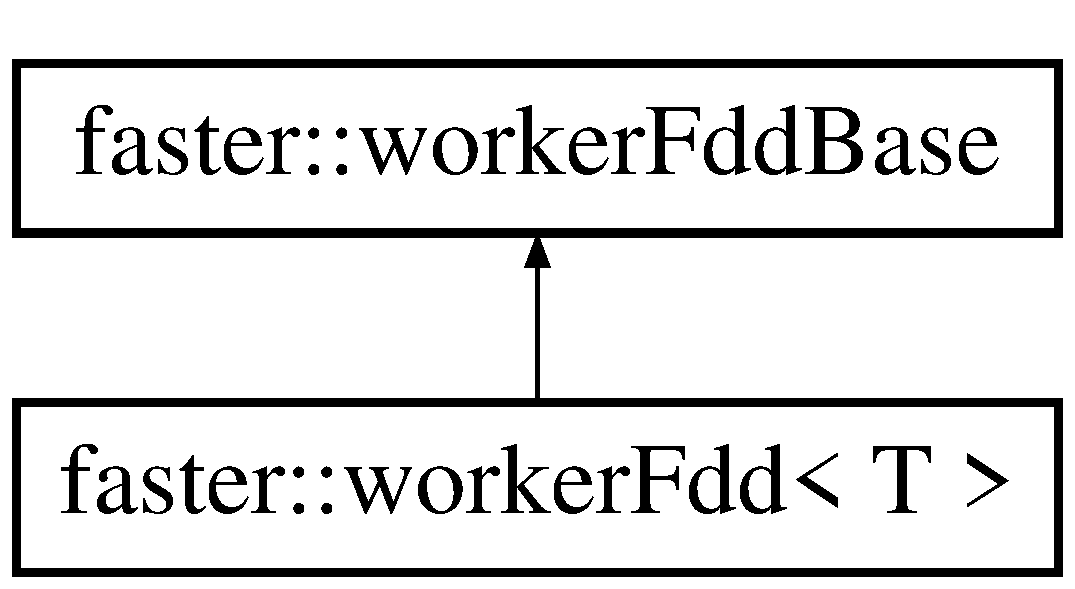
\includegraphics[height=2.000000cm]{classfaster_1_1workerFdd}
\end{center}
\end{figure}
\subsection*{Public Member Functions}
\begin{DoxyCompactItemize}
\item 
\hypertarget{classfaster_1_1workerFdd_a93ad6099e1b600358729aa45952c6ac9}{}{\bfseries worker\+Fdd} (fdd\+Type t)\label{classfaster_1_1workerFdd_a93ad6099e1b600358729aa45952c6ac9}

\item 
\hypertarget{classfaster_1_1workerFdd_aa07a10094bc1f054d2bb5fe89f3c2379}{}{\bfseries worker\+Fdd} (fdd\+Type kt, fdd\+Type t)\label{classfaster_1_1workerFdd_aa07a10094bc1f054d2bb5fe89f3c2379}

\item 
\hypertarget{classfaster_1_1workerFdd_a4d9f824ec396f44f4876f39f665c719b}{}{\bfseries worker\+Fdd} (unsigned long int ident, fdd\+Type t)\label{classfaster_1_1workerFdd_a4d9f824ec396f44f4876f39f665c719b}

\item 
\hypertarget{classfaster_1_1workerFdd_a592fd4bca2d66794987a8084c80e3248}{}{\bfseries worker\+Fdd} (unsigned long int ident, fdd\+Type t, size\+\_\+t size)\label{classfaster_1_1workerFdd_a592fd4bca2d66794987a8084c80e3248}

\item 
\hypertarget{classfaster_1_1workerFdd_af9f296569b13b1c548658eb083c86104}{}{\bfseries worker\+Fdd} (unsigned long int ident, fdd\+Type kt, fdd\+Type t)\label{classfaster_1_1workerFdd_af9f296569b13b1c548658eb083c86104}

\item 
\hypertarget{classfaster_1_1workerFdd_afc006b52499d50841f0a0aedd19331b3}{}{\bfseries worker\+Fdd} (unsigned long int ident, fdd\+Type kt, fdd\+Type t, size\+\_\+t size)\label{classfaster_1_1workerFdd_afc006b52499d50841f0a0aedd19331b3}

\item 
\hypertarget{classfaster_1_1workerFdd_ad994411caadedc41999bfc357dc96663}{}fdd\+Type {\bfseries get\+Type} ()\label{classfaster_1_1workerFdd_ad994411caadedc41999bfc357dc96663}

\item 
\hypertarget{classfaster_1_1workerFdd_a1f6f0608cd46a0f2ad53daa6ef3e9284}{}fdd\+Type {\bfseries get\+Key\+Type} ()\label{classfaster_1_1workerFdd_a1f6f0608cd46a0f2ad53daa6ef3e9284}

\item 
\hypertarget{classfaster_1_1workerFdd_a8794c182b3d3da254dabf54d0f9ce490}{}void $\ast$ {\bfseries get\+Item} (size\+\_\+t address)\label{classfaster_1_1workerFdd_a8794c182b3d3da254dabf54d0f9ce490}

\item 
\hypertarget{classfaster_1_1workerFdd_a848160e2971c286c7a3aad710dd0b9fb}{}void $\ast$ {\bfseries get\+Keys} ()\label{classfaster_1_1workerFdd_a848160e2971c286c7a3aad710dd0b9fb}

\item 
\hypertarget{classfaster_1_1workerFdd_a91445867b8280e20301e6e07e7afc6b2}{}void $\ast$ {\bfseries get\+Data} ()\label{classfaster_1_1workerFdd_a91445867b8280e20301e6e07e7afc6b2}

\item 
\hypertarget{classfaster_1_1workerFdd_acdedac95179fa5a2c4b88fb9c250acd6}{}size\+\_\+t {\bfseries get\+Size} ()\label{classfaster_1_1workerFdd_acdedac95179fa5a2c4b88fb9c250acd6}

\item 
\hypertarget{classfaster_1_1workerFdd_aac8ebab407dd4c0024700bb2ab7601d7}{}size\+\_\+t {\bfseries item\+Size} ()\label{classfaster_1_1workerFdd_aac8ebab407dd4c0024700bb2ab7601d7}

\item 
\hypertarget{classfaster_1_1workerFdd_a2e60538a409f44fa5fdaadcd9960508a}{}size\+\_\+t {\bfseries base\+Size} ()\label{classfaster_1_1workerFdd_a2e60538a409f44fa5fdaadcd9960508a}

\item 
\hypertarget{classfaster_1_1workerFdd_a1688e263591a30c9a715df234af3a631}{}void {\bfseries set\+Size} (size\+\_\+t s)\label{classfaster_1_1workerFdd_a1688e263591a30c9a715df234af3a631}

\item 
\hypertarget{classfaster_1_1workerFdd_ab25cae53f4ba6d2b5fbd9c0e7e1cbe06}{}void {\bfseries delete\+Item} (void $\ast$item)\label{classfaster_1_1workerFdd_ab25cae53f4ba6d2b5fbd9c0e7e1cbe06}

\item 
\hypertarget{classfaster_1_1workerFdd_ab38a9a23eff8164ce9b5c7e2bb617f99}{}void {\bfseries shrink} ()\label{classfaster_1_1workerFdd_ab38a9a23eff8164ce9b5c7e2bb617f99}

\item 
\hypertarget{classfaster_1_1workerFdd_ae22b78af425a3d3fb21af154614e8b20}{}void {\bfseries set\+Data} (void $\ast$d, size\+\_\+t size)\label{classfaster_1_1workerFdd_ae22b78af425a3d3fb21af154614e8b20}

\item 
\hypertarget{classfaster_1_1workerFdd_aeb6300f2d679b6b44693516d821c2b96}{}void {\bfseries set\+Data} (void $\ast$d, size\+\_\+t $\ast$line\+Sizes, size\+\_\+t size)\label{classfaster_1_1workerFdd_aeb6300f2d679b6b44693516d821c2b96}

\item 
\hypertarget{classfaster_1_1workerFdd_a168689aa68b6a02374d0f78ea0b2a3ed}{}void {\bfseries set\+Data} (void $\ast$k, void $\ast$d, size\+\_\+t size)\label{classfaster_1_1workerFdd_a168689aa68b6a02374d0f78ea0b2a3ed}

\item 
\hypertarget{classfaster_1_1workerFdd_ac399b11ae3a5a385acb52c2547baec51}{}void {\bfseries set\+Data} (void $\ast$k, void $\ast$d, size\+\_\+t $\ast$line\+Sizes, size\+\_\+t size)\label{classfaster_1_1workerFdd_ac399b11ae3a5a385acb52c2547baec51}

\item 
\hypertarget{classfaster_1_1workerFdd_abe1fe4ca054f914d12d2e24bd8ea49df}{}void {\bfseries set\+Data\+Raw} (void $\ast$data, size\+\_\+t size) override\label{classfaster_1_1workerFdd_abe1fe4ca054f914d12d2e24bd8ea49df}

\item 
\hypertarget{classfaster_1_1workerFdd_a60851f472a919037ae93c0ddf2fdbc4c}{}void {\bfseries set\+Data\+Raw} (void $\ast$data, size\+\_\+t $\ast$line\+Sizes, size\+\_\+t size)\label{classfaster_1_1workerFdd_a60851f472a919037ae93c0ddf2fdbc4c}

\item 
\hypertarget{classfaster_1_1workerFdd_af42e9fc7c5a824c63882b5fd6f494556}{}void {\bfseries set\+Data\+Raw} (void $\ast$k, void $\ast$d, size\+\_\+t s)\label{classfaster_1_1workerFdd_af42e9fc7c5a824c63882b5fd6f494556}

\item 
\hypertarget{classfaster_1_1workerFdd_a3247e1b4c7f74766d8f9bfb95ec35783}{}void {\bfseries set\+Data\+Raw} (void $\ast$k, void $\ast$d, size\+\_\+t $\ast$l, size\+\_\+t s)\label{classfaster_1_1workerFdd_a3247e1b4c7f74766d8f9bfb95ec35783}

\item 
\hypertarget{classfaster_1_1workerFdd_a7b11ae170c7047bcefdf58bfac27b605}{}size\+\_\+t $\ast$ {\bfseries get\+Line\+Sizes} ()\label{classfaster_1_1workerFdd_a7b11ae170c7047bcefdf58bfac27b605}

\item 
\hypertarget{classfaster_1_1workerFdd_a168e376cf191c14355f748526861962c}{}void {\bfseries insert} (void $\ast$k, void $\ast$in, size\+\_\+t s)\label{classfaster_1_1workerFdd_a168e376cf191c14355f748526861962c}

\item 
\hypertarget{classfaster_1_1workerFdd_af4ce92cd1a88a5a568df4cb8dd3429ae}{}void {\bfseries insertl} (void $\ast$in)\label{classfaster_1_1workerFdd_af4ce92cd1a88a5a568df4cb8dd3429ae}

\item 
\hypertarget{classfaster_1_1workerFdd_a7b54fa501fd3cd31a27b95cc55b6235a}{}void {\bfseries apply} (void $\ast$func U\+N\+U\+S\+E\+D, fdd\+Op\+Type op U\+N\+U\+S\+E\+D, \hyperlink{classfaster_1_1workerFddBase}{worker\+Fdd\+Base} $\ast$dest U\+N\+U\+S\+E\+D, \hyperlink{classfaster_1_1fastCommBuffer}{fast\+Comm\+Buffer} \&comm U\+N\+U\+S\+E\+D)\label{classfaster_1_1workerFdd_a7b54fa501fd3cd31a27b95cc55b6235a}

\item 
\hypertarget{classfaster_1_1workerFdd_a245c74dd6908a15c8e4310e21c25f867}{}void {\bfseries preapply} (unsigned long int id, void $\ast$func, fdd\+Op\+Type op, \hyperlink{classfaster_1_1workerFddBase}{worker\+Fdd\+Base} $\ast$dest, \hyperlink{classfaster_1_1fastComm}{fast\+Comm} $\ast$comm) override\label{classfaster_1_1workerFdd_a245c74dd6908a15c8e4310e21c25f867}

\item 
\hypertarget{classfaster_1_1workerFdd_a429828080212db643940e5761b9bc27c}{}void {\bfseries collect} (\hyperlink{classfaster_1_1fastComm}{fast\+Comm} $\ast$comm) override\label{classfaster_1_1workerFdd_a429828080212db643940e5761b9bc27c}

\item 
\hypertarget{classfaster_1_1workerFdd_a4e4649c682140139aa4d8e7612086bfd}{}void {\bfseries group\+By\+Key} (\hyperlink{classfaster_1_1fastComm}{fast\+Comm} $\ast$comm)\label{classfaster_1_1workerFdd_a4e4649c682140139aa4d8e7612086bfd}

\item 
\hypertarget{classfaster_1_1workerFdd_a4be02069920848e005273f560e99b3c8}{}void {\bfseries count\+By\+Key} (\hyperlink{classfaster_1_1fastComm}{fast\+Comm} $\ast$comm)\label{classfaster_1_1workerFdd_a4be02069920848e005273f560e99b3c8}

\item 
\hypertarget{classfaster_1_1workerFdd_a125d58b5669006099a3ce4fd7042413a}{}void {\bfseries exchange\+Data\+By\+Key} (\hyperlink{classfaster_1_1fastComm}{fast\+Comm} $\ast$comm, void $\ast$key\+Map)\label{classfaster_1_1workerFdd_a125d58b5669006099a3ce4fd7042413a}

\item 
\hypertarget{classfaster_1_1workerFdd_a65f3935109ac34d4533d6b8bdc7a049e}{}std\+::vector$<$ std\+::vector$<$ void $\ast$ $>$ $>$ $\ast$ {\bfseries get\+Key\+Locations} ()\label{classfaster_1_1workerFdd_a65f3935109ac34d4533d6b8bdc7a049e}

\end{DoxyCompactItemize}
\subsection*{Additional Inherited Members}


The documentation for this class was generated from the following files\+:\begin{DoxyCompactItemize}
\item 
/home/mtcs/pesquisa/faster/faster.\+git/src/include/\+\_\+worker\+Fdd.\+h\item 
/home/mtcs/pesquisa/faster/faster.\+git/src/include/worker\+Fdd.\+h\end{DoxyCompactItemize}

\hypertarget{classfaster_1_1workerFddBase}{}\section{faster\+:\+:worker\+Fdd\+Base Class Reference}
\label{classfaster_1_1workerFddBase}\index{faster\+::worker\+Fdd\+Base@{faster\+::worker\+Fdd\+Base}}
Inheritance diagram for faster\+:\+:worker\+Fdd\+Base\+:\begin{figure}[H]
\begin{center}
\leavevmode
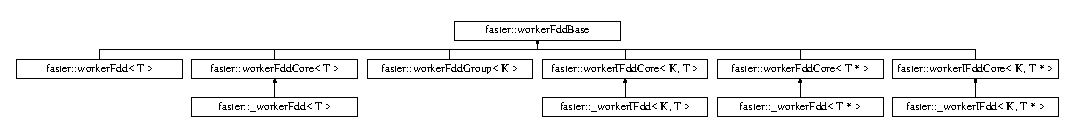
\includegraphics[height=1.333333cm]{classfaster_1_1workerFddBase}
\end{center}
\end{figure}
\subsection*{Public Member Functions}
\begin{DoxyCompactItemize}
\item 
\hypertarget{classfaster_1_1workerFddBase_a8e25e46286deed01d3131e2ac7fb7560}{}{\bfseries worker\+Fdd\+Base} (unsigned int ident, fdd\+Type t)\label{classfaster_1_1workerFddBase_a8e25e46286deed01d3131e2ac7fb7560}

\item 
\hypertarget{classfaster_1_1workerFddBase_a60a32cfcbe768ca3ffa64b98389441ee}{}virtual fdd\+Type {\bfseries get\+Type} ()=0\label{classfaster_1_1workerFddBase_a60a32cfcbe768ca3ffa64b98389441ee}

\item 
\hypertarget{classfaster_1_1workerFddBase_aece939bd2cd9652a7fb49d2dca865e3d}{}virtual fdd\+Type {\bfseries get\+Key\+Type} ()=0\label{classfaster_1_1workerFddBase_aece939bd2cd9652a7fb49d2dca865e3d}

\item 
\hypertarget{classfaster_1_1workerFddBase_a325bd99069264118804eb29ef808d37c}{}virtual void {\bfseries set\+Data} (void $\ast$, size\+\_\+t)=0\label{classfaster_1_1workerFddBase_a325bd99069264118804eb29ef808d37c}

\item 
\hypertarget{classfaster_1_1workerFddBase_a7301d03d82d61aae044b1e53d1595338}{}virtual void {\bfseries set\+Data} (void $\ast$, size\+\_\+t $\ast$, size\+\_\+t)=0\label{classfaster_1_1workerFddBase_a7301d03d82d61aae044b1e53d1595338}

\item 
\hypertarget{classfaster_1_1workerFddBase_ab3de9c6bb71c998d51482be316da4dce}{}virtual void {\bfseries set\+Data} (void $\ast$, void $\ast$, size\+\_\+t)=0\label{classfaster_1_1workerFddBase_ab3de9c6bb71c998d51482be316da4dce}

\item 
\hypertarget{classfaster_1_1workerFddBase_aa80255f187115a003f2e869366ecb6b6}{}virtual void {\bfseries set\+Data} (void $\ast$, void $\ast$, size\+\_\+t $\ast$, size\+\_\+t)=0\label{classfaster_1_1workerFddBase_aa80255f187115a003f2e869366ecb6b6}

\item 
\hypertarget{classfaster_1_1workerFddBase_ac02bc5670916dd922ea8d5c505b08899}{}virtual void {\bfseries set\+Data\+Raw} (void $\ast$, size\+\_\+t)=0\label{classfaster_1_1workerFddBase_ac02bc5670916dd922ea8d5c505b08899}

\item 
\hypertarget{classfaster_1_1workerFddBase_acb1d91424c30dfc596b2e437605fa613}{}virtual void {\bfseries set\+Data\+Raw} (void $\ast$, size\+\_\+t $\ast$, size\+\_\+t)=0\label{classfaster_1_1workerFddBase_acb1d91424c30dfc596b2e437605fa613}

\item 
\hypertarget{classfaster_1_1workerFddBase_a9a6dd9e0a89281b14486c685ff15d22b}{}virtual void {\bfseries set\+Data\+Raw} (void $\ast$, void $\ast$, size\+\_\+t)=0\label{classfaster_1_1workerFddBase_a9a6dd9e0a89281b14486c685ff15d22b}

\item 
\hypertarget{classfaster_1_1workerFddBase_a5d73e6097368101ce3af5eef1309bdff}{}virtual void {\bfseries set\+Data\+Raw} (void $\ast$, void $\ast$, size\+\_\+t $\ast$, size\+\_\+t)=0\label{classfaster_1_1workerFddBase_a5d73e6097368101ce3af5eef1309bdff}

\item 
\hypertarget{classfaster_1_1workerFddBase_a602b1ad564266ed18e873e24f1418e1b}{}virtual void $\ast$ {\bfseries get\+Item} (size\+\_\+t)=0\label{classfaster_1_1workerFddBase_a602b1ad564266ed18e873e24f1418e1b}

\item 
\hypertarget{classfaster_1_1workerFddBase_a65ea9b06048b3cef3757aec9738ec07f}{}virtual void $\ast$ {\bfseries get\+Keys} ()=0\label{classfaster_1_1workerFddBase_a65ea9b06048b3cef3757aec9738ec07f}

\item 
\hypertarget{classfaster_1_1workerFddBase_af315b09bb75b414d4840c4d0fd3d307f}{}virtual void $\ast$ {\bfseries get\+Data} ()=0\label{classfaster_1_1workerFddBase_af315b09bb75b414d4840c4d0fd3d307f}

\item 
\hypertarget{classfaster_1_1workerFddBase_ab3b64bebf2d7046a583b1e391ba69d1a}{}virtual size\+\_\+t {\bfseries get\+Size} ()=0\label{classfaster_1_1workerFddBase_ab3b64bebf2d7046a583b1e391ba69d1a}

\item 
\hypertarget{classfaster_1_1workerFddBase_a9ae5dce20da30fb989599257ab940bf8}{}virtual size\+\_\+t $\ast$ {\bfseries get\+Line\+Sizes} ()=0\label{classfaster_1_1workerFddBase_a9ae5dce20da30fb989599257ab940bf8}

\item 
\hypertarget{classfaster_1_1workerFddBase_ad0ce609bfa4571280c01ff618b2f6706}{}virtual void {\bfseries set\+Size} (size\+\_\+t s)=0\label{classfaster_1_1workerFddBase_ad0ce609bfa4571280c01ff618b2f6706}

\item 
\hypertarget{classfaster_1_1workerFddBase_a11e77f238c760ce939ceeaa7f36a7899}{}virtual size\+\_\+t {\bfseries item\+Size} ()=0\label{classfaster_1_1workerFddBase_a11e77f238c760ce939ceeaa7f36a7899}

\item 
\hypertarget{classfaster_1_1workerFddBase_adf7e8dd9728b866d37bc32aeba4e7c3c}{}virtual size\+\_\+t {\bfseries base\+Size} ()=0\label{classfaster_1_1workerFddBase_adf7e8dd9728b866d37bc32aeba4e7c3c}

\item 
\hypertarget{classfaster_1_1workerFddBase_aac667e68629f17c9c5cd30bf9701f03c}{}virtual void {\bfseries delete\+Item} (void $\ast$item)=0\label{classfaster_1_1workerFddBase_aac667e68629f17c9c5cd30bf9701f03c}

\item 
\hypertarget{classfaster_1_1workerFddBase_afd958be3b502d6147e3145c4d2926452}{}virtual void {\bfseries shrink} ()=0\label{classfaster_1_1workerFddBase_afd958be3b502d6147e3145c4d2926452}

\item 
\hypertarget{classfaster_1_1workerFddBase_a7e2a919ffa1ecd117c2d487957f9e431}{}virtual void {\bfseries insertl} (void $\ast$v)=0\label{classfaster_1_1workerFddBase_a7e2a919ffa1ecd117c2d487957f9e431}

\item 
\hypertarget{classfaster_1_1workerFddBase_adef4d0ad067b5bc9ca39d21260b46818}{}virtual void {\bfseries insert} (void $\ast$k, void $\ast$v, size\+\_\+t s)=0\label{classfaster_1_1workerFddBase_adef4d0ad067b5bc9ca39d21260b46818}

\item 
\hypertarget{classfaster_1_1workerFddBase_a6dbb190837ac0eecf4c2a4b4c3f95920}{}virtual void {\bfseries preapply} (unsigned long int id, void $\ast$func, fdd\+Op\+Type op, \hyperlink{classfaster_1_1workerFddBase}{worker\+Fdd\+Base} $\ast$dest, \hyperlink{classfaster_1_1fastComm}{fast\+Comm} $\ast$comm)=0\label{classfaster_1_1workerFddBase_a6dbb190837ac0eecf4c2a4b4c3f95920}

\item 
\hypertarget{classfaster_1_1workerFddBase_a875b78e89873f4b4b88611f8e1127baa}{}virtual void {\bfseries apply} (void $\ast$func, fdd\+Op\+Type op, \hyperlink{classfaster_1_1workerFddBase}{worker\+Fdd\+Base} $\ast$dest, \hyperlink{classfaster_1_1fastCommBuffer}{fast\+Comm\+Buffer} \&buffer)=0\label{classfaster_1_1workerFddBase_a875b78e89873f4b4b88611f8e1127baa}

\item 
\hypertarget{classfaster_1_1workerFddBase_ab9f9ea54f3480513b53e40760399e569}{}virtual void {\bfseries collect} (\hyperlink{classfaster_1_1fastComm}{fast\+Comm} $\ast$comm)=0\label{classfaster_1_1workerFddBase_ab9f9ea54f3480513b53e40760399e569}

\item 
\hypertarget{classfaster_1_1workerFddBase_a4a9b7afbb072da590bd5d93e46d1052a}{}virtual void {\bfseries exchange\+Data\+By\+Key} (\hyperlink{classfaster_1_1fastComm}{fast\+Comm} $\ast$comm, void $\ast$key\+Map)=0\label{classfaster_1_1workerFddBase_a4a9b7afbb072da590bd5d93e46d1052a}

\item 
\hypertarget{classfaster_1_1workerFddBase_a7ceebadaee829b6c3c8e247060abc41d}{}virtual std\+::vector$<$ std\+::vector$<$ void $\ast$ $>$ $>$ $\ast$ {\bfseries get\+Key\+Locations} ()=0\label{classfaster_1_1workerFddBase_a7ceebadaee829b6c3c8e247060abc41d}

\end{DoxyCompactItemize}
\subsection*{Protected Attributes}
\begin{DoxyCompactItemize}
\item 
\hypertarget{classfaster_1_1workerFddBase_ab131549612a7a269aab35c1920f0e215}{}unsigned long int {\bfseries id}\label{classfaster_1_1workerFddBase_ab131549612a7a269aab35c1920f0e215}

\item 
\hypertarget{classfaster_1_1workerFddBase_a220b88e4e5633d9ee7c8c8697a9ff297}{}fdd\+Type {\bfseries type}\label{classfaster_1_1workerFddBase_a220b88e4e5633d9ee7c8c8697a9ff297}

\item 
\hypertarget{classfaster_1_1workerFddBase_ab5d502564e1c1b12e806033380431afb}{}fdd\+Type {\bfseries key\+Type}\label{classfaster_1_1workerFddBase_ab5d502564e1c1b12e806033380431afb}

\end{DoxyCompactItemize}


The documentation for this class was generated from the following files\+:\begin{DoxyCompactItemize}
\item 
/home/mtcs/pesquisa/faster/faster.\+git/src/include/worker\+Fdd\+Base.\+h\item 
/home/mtcs/pesquisa/faster/faster.\+git/src/libfaster/worker\+Fdd\+Base.\+cpp\end{DoxyCompactItemize}

\hypertarget{classfaster_1_1workerFddCore}{}\section{faster\+:\+:worker\+Fdd\+Core$<$ T $>$ Class Template Reference}
\label{classfaster_1_1workerFddCore}\index{faster\+::worker\+Fdd\+Core$<$ T $>$@{faster\+::worker\+Fdd\+Core$<$ T $>$}}
Inheritance diagram for faster\+:\+:worker\+Fdd\+Core$<$ T $>$\+:\begin{figure}[H]
\begin{center}
\leavevmode
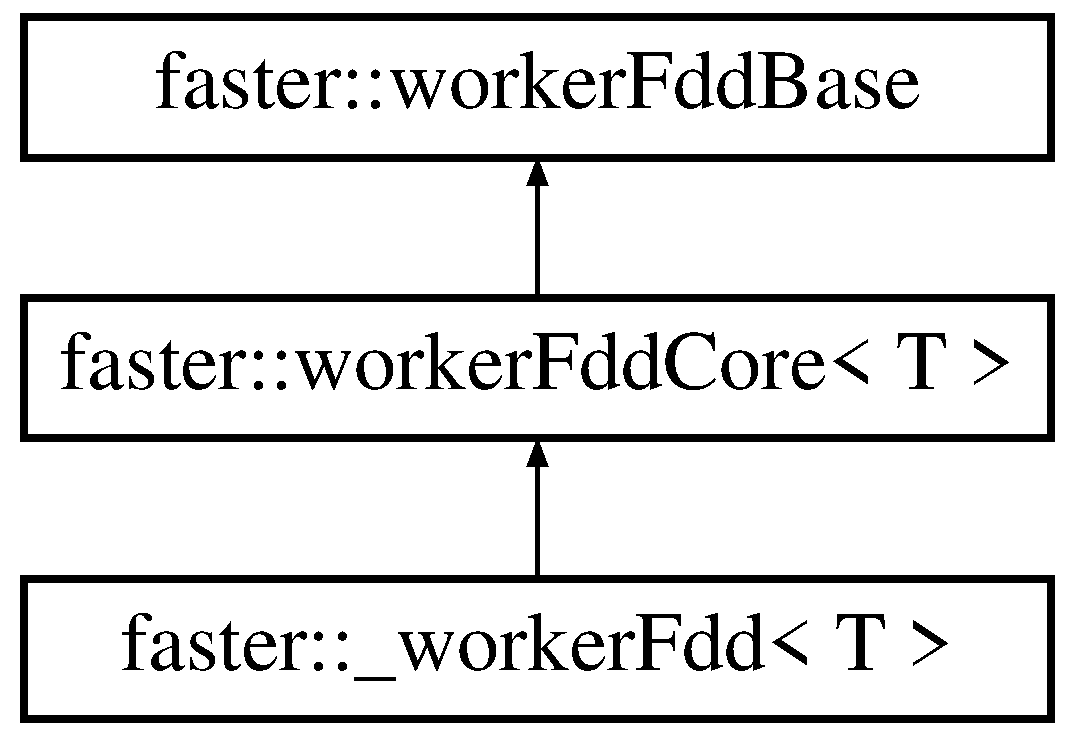
\includegraphics[height=3.000000cm]{classfaster_1_1workerFddCore}
\end{center}
\end{figure}
\subsection*{Public Member Functions}
\begin{DoxyCompactItemize}
\item 
\hypertarget{classfaster_1_1workerFddCore_a83405d10b12b6a2c52e05ce6aa154a58}{}\label{classfaster_1_1workerFddCore_a83405d10b12b6a2c52e05ce6aa154a58} 
{\bfseries worker\+Fdd\+Core} (unsigned int ident, \hyperlink{namespacefaster_aa8898687bc64536b60a3d5f365060cd6}{fdd\+Type} t)
\item 
\hypertarget{classfaster_1_1workerFddCore_a916e1e6320f5d65f876ea8a13b8e4962}{}\label{classfaster_1_1workerFddCore_a916e1e6320f5d65f876ea8a13b8e4962} 
{\bfseries worker\+Fdd\+Core} (unsigned int ident, \hyperlink{namespacefaster_aa8898687bc64536b60a3d5f365060cd6}{fdd\+Type} t, size\+\_\+t size)
\item 
\hypertarget{classfaster_1_1workerFddCore_aadc1b6c29965af371b2c6b3f246108f6}{}\label{classfaster_1_1workerFddCore_aadc1b6c29965af371b2c6b3f246108f6} 
void {\bfseries set\+Data} (void $\ast$k U\+N\+U\+S\+ED, void $\ast$d U\+N\+U\+S\+ED, size\+\_\+t size U\+N\+U\+S\+ED)
\item 
\hypertarget{classfaster_1_1workerFddCore_ad18325128eb5c84bf1ce2c14dd885ec8}{}\label{classfaster_1_1workerFddCore_ad18325128eb5c84bf1ce2c14dd885ec8} 
void {\bfseries set\+Data\+Raw} (void $\ast$keys U\+N\+U\+S\+ED, void $\ast$data U\+N\+U\+S\+ED, size\+\_\+t size U\+N\+U\+S\+ED) override
\item 
\hypertarget{classfaster_1_1workerFddCore_ac41afe052888d211137a09702ab19ac8}{}\label{classfaster_1_1workerFddCore_ac41afe052888d211137a09702ab19ac8} 
void {\bfseries set\+Data\+Raw} (void $\ast$keys U\+N\+U\+S\+ED, void $\ast$data U\+N\+U\+S\+ED, size\+\_\+t $\ast$line\+Sizes U\+N\+U\+S\+ED, size\+\_\+t size U\+N\+U\+S\+ED) override
\item 
\hypertarget{classfaster_1_1workerFddCore_a76c12aa66cb7baebdb63688f7599dd41}{}\label{classfaster_1_1workerFddCore_a76c12aa66cb7baebdb63688f7599dd41} 
\hyperlink{namespacefaster_aa8898687bc64536b60a3d5f365060cd6}{fdd\+Type} {\bfseries get\+Type} () override
\item 
\hypertarget{classfaster_1_1workerFddCore_a2782ab77ddb4a72cf4f84af84072efba}{}\label{classfaster_1_1workerFddCore_a2782ab77ddb4a72cf4f84af84072efba} 
\hyperlink{namespacefaster_aa8898687bc64536b60a3d5f365060cd6}{fdd\+Type} {\bfseries get\+Key\+Type} () override
\item 
\hypertarget{classfaster_1_1workerFddCore_ad93c9c3c5836ab3bf5a8bc425d976211}{}\label{classfaster_1_1workerFddCore_ad93c9c3c5836ab3bf5a8bc425d976211} 
T \& {\bfseries operator\mbox{[}$\,$\mbox{]}} (size\+\_\+t address)
\item 
\hypertarget{classfaster_1_1workerFddCore_a7753b4b41fa7c87676f7a6ef75a125cb}{}\label{classfaster_1_1workerFddCore_a7753b4b41fa7c87676f7a6ef75a125cb} 
void $\ast$ {\bfseries get\+Item} (size\+\_\+t address)
\item 
\hypertarget{classfaster_1_1workerFddCore_ae3768cc9c330c25c669611b5df3c5454}{}\label{classfaster_1_1workerFddCore_ae3768cc9c330c25c669611b5df3c5454} 
void $\ast$ {\bfseries get\+Keys} () override
\item 
\hypertarget{classfaster_1_1workerFddCore_a77172c15f3409bbe233be13aabfe8071}{}\label{classfaster_1_1workerFddCore_a77172c15f3409bbe233be13aabfe8071} 
void $\ast$ {\bfseries get\+Data} () override
\item 
\hypertarget{classfaster_1_1workerFddCore_a32bd4aca33e352d018a3bde34e7104d2}{}\label{classfaster_1_1workerFddCore_a32bd4aca33e352d018a3bde34e7104d2} 
size\+\_\+t {\bfseries get\+Size} () override
\item 
\hypertarget{classfaster_1_1workerFddCore_a68f16ce63e3bda36270a9f096e7bf007}{}\label{classfaster_1_1workerFddCore_a68f16ce63e3bda36270a9f096e7bf007} 
size\+\_\+t {\bfseries item\+Size} () override
\item 
\hypertarget{classfaster_1_1workerFddCore_aa56e4f3c789781c5e5745cb1a9f55032}{}\label{classfaster_1_1workerFddCore_aa56e4f3c789781c5e5745cb1a9f55032} 
size\+\_\+t {\bfseries base\+Size} () override
\item 
\hypertarget{classfaster_1_1workerFddCore_ae6834075d00c10b68b4ed8dc56a43ff1}{}\label{classfaster_1_1workerFddCore_ae6834075d00c10b68b4ed8dc56a43ff1} 
void {\bfseries set\+Size} (size\+\_\+t s)
\item 
\hypertarget{classfaster_1_1workerFddCore_aece15833d979a1315018b17426f9f943}{}\label{classfaster_1_1workerFddCore_aece15833d979a1315018b17426f9f943} 
void {\bfseries delete\+Item} (void $\ast$item) override
\item 
\hypertarget{classfaster_1_1workerFddCore_a9e9247a366e0a1e1b60c759ff9badb5c}{}\label{classfaster_1_1workerFddCore_a9e9247a366e0a1e1b60c759ff9badb5c} 
void {\bfseries shrink} ()
\item 
\hypertarget{classfaster_1_1workerFddCore_aba13e77488bcc84daaed00c0fb899eae}{}\label{classfaster_1_1workerFddCore_aba13e77488bcc84daaed00c0fb899eae} 
void {\bfseries write\+To\+File} (void $\ast$path, size\+\_\+t proc\+Id, void $\ast$sufix)
\item 
\hypertarget{classfaster_1_1workerFddCore_a4533454652b609e0cedb026ad1d3e881}{}\label{classfaster_1_1workerFddCore_a4533454652b609e0cedb026ad1d3e881} 
void {\bfseries preapply} (unsigned long int id, void $\ast$func, \hyperlink{namespacefaster_a64379512d12d41c6e58f176939abfd80}{fdd\+Op\+Type} op, \hyperlink{classfaster_1_1workerFddBase}{worker\+Fdd\+Base} $\ast$dest, \hyperlink{classfaster_1_1fastComm}{fast\+Comm} $\ast$comm)
\end{DoxyCompactItemize}
\subsection*{Protected Member Functions}
\begin{DoxyCompactItemize}
\item 
\hypertarget{classfaster_1_1workerFddCore_a970f3471f714c359c0b9d7f50711726a}{}\label{classfaster_1_1workerFddCore_a970f3471f714c359c0b9d7f50711726a} 
void {\bfseries exchange\+Data\+By\+Key} (\hyperlink{classfaster_1_1fastComm}{fast\+Comm} $\ast$comm U\+N\+U\+S\+ED)
\item 
\hypertarget{classfaster_1_1workerFddCore_a680e4cf4f9702680b2c2d510798a3166}{}\label{classfaster_1_1workerFddCore_a680e4cf4f9702680b2c2d510798a3166} 
void $\ast$ {\bfseries get\+U\+Keys} ()
\item 
\hypertarget{classfaster_1_1workerFddCore_a79f382d37ac47873306241217b51e1e6}{}\label{classfaster_1_1workerFddCore_a79f382d37ac47873306241217b51e1e6} 
void {\bfseries set\+U\+Keys} (void $\ast$uk U\+N\+U\+S\+ED)
\item 
\hypertarget{classfaster_1_1workerFddCore_acb4598d5ac4ae60c646ab72f26d05db8}{}\label{classfaster_1_1workerFddCore_acb4598d5ac4ae60c646ab72f26d05db8} 
void $\ast$ {\bfseries get\+Key\+Map} ()
\item 
\hypertarget{classfaster_1_1workerFddCore_a27bcb7913c94c74f0b6254456db0265a}{}\label{classfaster_1_1workerFddCore_a27bcb7913c94c74f0b6254456db0265a} 
void {\bfseries set\+Key\+Map} (void $\ast$km U\+N\+U\+S\+ED)
\item 
\hypertarget{classfaster_1_1workerFddCore_a8b82124f0cf058974f73df7521a1aa80}{}\label{classfaster_1_1workerFddCore_a8b82124f0cf058974f73df7521a1aa80} 
std\+::vector$<$ std\+::vector$<$ void $\ast$ $>$ $>$ $\ast$ {\bfseries get\+Key\+Locations} ()
\end{DoxyCompactItemize}
\subsection*{Protected Attributes}
\begin{DoxyCompactItemize}
\item 
\hypertarget{classfaster_1_1workerFddCore_aba24c5db034dd1b8235b9ad4483c5e0e}{}\label{classfaster_1_1workerFddCore_aba24c5db034dd1b8235b9ad4483c5e0e} 
\hyperlink{classfaster_1_1fddStorage}{fdd\+Storage}$<$ T $>$ $\ast$ {\bfseries local\+Data}
\end{DoxyCompactItemize}


The documentation for this class was generated from the following files\+:\begin{DoxyCompactItemize}
\item 
/home/mtcs/pesquisa/faster/faster.\+git/src/include/\+\_\+worker\+Fdd.\+h\item 
/home/mtcs/pesquisa/faster/faster.\+git/src/libfaster/worker\+Fdd\+Core.\+cpp\end{DoxyCompactItemize}

\hypertarget{classfaster_1_1workerFddGroup}{}\section{faster\+:\+:worker\+Fdd\+Group$<$ K $>$ Class Template Reference}
\label{classfaster_1_1workerFddGroup}\index{faster\+::worker\+Fdd\+Group$<$ K $>$@{faster\+::worker\+Fdd\+Group$<$ K $>$}}
Inheritance diagram for faster\+:\+:worker\+Fdd\+Group$<$ K $>$\+:\begin{figure}[H]
\begin{center}
\leavevmode
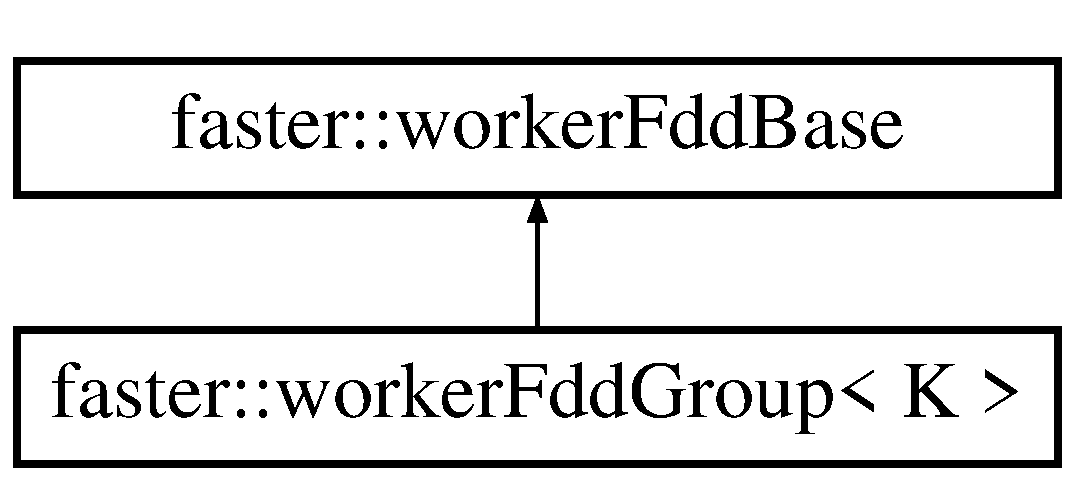
\includegraphics[height=2.000000cm]{classfaster_1_1workerFddGroup}
\end{center}
\end{figure}


\subsection{Description}
\subsubsection*{template$<$typename K$>$\newline
class faster\+::worker\+Fdd\+Group$<$ K $>$}



Definition at line 14 of file worker\+Fdd\+Group.\+h.

\subsection*{Public Member Functions}
\begin{DoxyCompactItemize}
\item 
\hypertarget{classfaster_1_1workerFddGroup_ad925b72158482f9cdf8d84159fc4ed53}{}\label{classfaster_1_1workerFddGroup_ad925b72158482f9cdf8d84159fc4ed53} 
{\bfseries worker\+Fdd\+Group} (unsigned long int id, \hyperlink{namespacefaster_aa8898687bc64536b60a3d5f365060cd6}{fdd\+Type} keyT, std\+::vector$<$ \hyperlink{classfaster_1_1workerFddBase}{worker\+Fdd\+Base} $\ast$$>$ \&members)
\item 
\hypertarget{classfaster_1_1workerFddGroup_ae63a674f1aa32f94ad52c364923694b1}{}\label{classfaster_1_1workerFddGroup_ae63a674f1aa32f94ad52c364923694b1} 
\hyperlink{namespacefaster_aa8898687bc64536b60a3d5f365060cd6}{fdd\+Type} {\bfseries get\+Type} ()
\item 
\hypertarget{classfaster_1_1workerFddGroup_abc818de0a5d3dee42a947318171101e3}{}\label{classfaster_1_1workerFddGroup_abc818de0a5d3dee42a947318171101e3} 
\hyperlink{namespacefaster_aa8898687bc64536b60a3d5f365060cd6}{fdd\+Type} {\bfseries get\+Key\+Type} ()
\item 
\hypertarget{classfaster_1_1workerFddGroup_a6dbf3389af39d6a3bdf172a8cf38a476}{}\label{classfaster_1_1workerFddGroup_a6dbf3389af39d6a3bdf172a8cf38a476} 
void {\bfseries set\+Data} (void $\ast$d U\+N\+U\+S\+ED, size\+\_\+t s U\+N\+U\+S\+ED)
\item 
\hypertarget{classfaster_1_1workerFddGroup_ab2e537d9dd20658236084d1d97ded324}{}\label{classfaster_1_1workerFddGroup_ab2e537d9dd20658236084d1d97ded324} 
void {\bfseries set\+Data} (void $\ast$d U\+N\+U\+S\+ED, size\+\_\+t $\ast$ds U\+N\+U\+S\+ED, size\+\_\+t s U\+N\+U\+S\+ED)
\item 
\hypertarget{classfaster_1_1workerFddGroup_a40b698ad7823ceb2ffab2fd7dca1f7bd}{}\label{classfaster_1_1workerFddGroup_a40b698ad7823ceb2ffab2fd7dca1f7bd} 
void {\bfseries set\+Data} (void $\ast$k U\+N\+U\+S\+ED, void $\ast$d U\+N\+U\+S\+ED, size\+\_\+t s U\+N\+U\+S\+ED)
\item 
\hypertarget{classfaster_1_1workerFddGroup_abadd56f253ffbdaf46b38f6e3c2e708a}{}\label{classfaster_1_1workerFddGroup_abadd56f253ffbdaf46b38f6e3c2e708a} 
void {\bfseries set\+Data} (void $\ast$k U\+N\+U\+S\+ED, void $\ast$d U\+N\+U\+S\+ED, size\+\_\+t $\ast$ds U\+N\+U\+S\+ED, size\+\_\+t s U\+N\+U\+S\+ED)
\item 
\hypertarget{classfaster_1_1workerFddGroup_add1d3823a8740b3b19fd223255e82193}{}\label{classfaster_1_1workerFddGroup_add1d3823a8740b3b19fd223255e82193} 
void {\bfseries set\+Data\+Raw} (void $\ast$d U\+N\+U\+S\+ED, size\+\_\+t s U\+N\+U\+S\+ED)
\item 
\hypertarget{classfaster_1_1workerFddGroup_af6caca6f3f898b13eb6d215d263f9ffd}{}\label{classfaster_1_1workerFddGroup_af6caca6f3f898b13eb6d215d263f9ffd} 
void {\bfseries set\+Data\+Raw} (void $\ast$d U\+N\+U\+S\+ED, size\+\_\+t $\ast$ds U\+N\+U\+S\+ED, size\+\_\+t s U\+N\+U\+S\+ED)
\item 
\hypertarget{classfaster_1_1workerFddGroup_aedb268724ef26a2b2983e4bea3888e86}{}\label{classfaster_1_1workerFddGroup_aedb268724ef26a2b2983e4bea3888e86} 
void {\bfseries set\+Data\+Raw} (void $\ast$k U\+N\+U\+S\+ED, void $\ast$d U\+N\+U\+S\+ED, size\+\_\+t s U\+N\+U\+S\+ED)
\item 
\hypertarget{classfaster_1_1workerFddGroup_ad4a8247e1a94473a93967b7e7f86e8d1}{}\label{classfaster_1_1workerFddGroup_ad4a8247e1a94473a93967b7e7f86e8d1} 
void {\bfseries set\+Data\+Raw} (void $\ast$k U\+N\+U\+S\+ED, void $\ast$d U\+N\+U\+S\+ED, size\+\_\+t $\ast$ds U\+N\+U\+S\+ED, size\+\_\+t s U\+N\+U\+S\+ED)
\item 
\hypertarget{classfaster_1_1workerFddGroup_a1bce4be21f1897e9646aa986fb58e644}{}\label{classfaster_1_1workerFddGroup_a1bce4be21f1897e9646aa986fb58e644} 
void $\ast$ {\bfseries get\+Item} (size\+\_\+t U\+N\+U\+S\+ED p)
\item 
\hypertarget{classfaster_1_1workerFddGroup_ade2366aef3d5772b81d6e9f9db9e05f2}{}\label{classfaster_1_1workerFddGroup_ade2366aef3d5772b81d6e9f9db9e05f2} 
void $\ast$ {\bfseries get\+Keys} ()
\item 
\hypertarget{classfaster_1_1workerFddGroup_a53c9d527b6488cb4fb649cbcade8ff92}{}\label{classfaster_1_1workerFddGroup_a53c9d527b6488cb4fb649cbcade8ff92} 
void $\ast$ {\bfseries get\+Data} ()
\item 
\hypertarget{classfaster_1_1workerFddGroup_a0337630f440733b964f5983195ba2d68}{}\label{classfaster_1_1workerFddGroup_a0337630f440733b964f5983195ba2d68} 
size\+\_\+t {\bfseries get\+Size} ()
\item 
\hypertarget{classfaster_1_1workerFddGroup_a65f2c1921dada1e313b6526f1eb01699}{}\label{classfaster_1_1workerFddGroup_a65f2c1921dada1e313b6526f1eb01699} 
size\+\_\+t $\ast$ {\bfseries get\+Line\+Sizes} ()
\item 
\hypertarget{classfaster_1_1workerFddGroup_af1c4980540ba874a02ccc4e428ffd7ff}{}\label{classfaster_1_1workerFddGroup_af1c4980540ba874a02ccc4e428ffd7ff} 
void {\bfseries set\+Size} (size\+\_\+t s U\+N\+U\+S\+ED)
\item 
\hypertarget{classfaster_1_1workerFddGroup_a41306315961dccb544e727bfea4ca84b}{}\label{classfaster_1_1workerFddGroup_a41306315961dccb544e727bfea4ca84b} 
size\+\_\+t {\bfseries item\+Size} ()
\item 
\hypertarget{classfaster_1_1workerFddGroup_a1299273f1bd2d218a67c9be41c2bafb8}{}\label{classfaster_1_1workerFddGroup_a1299273f1bd2d218a67c9be41c2bafb8} 
size\+\_\+t {\bfseries base\+Size} ()
\item 
\hypertarget{classfaster_1_1workerFddGroup_a7f786e4807bd56a4c04281756c417493}{}\label{classfaster_1_1workerFddGroup_a7f786e4807bd56a4c04281756c417493} 
void {\bfseries delete\+Item} (void $\ast$item U\+N\+U\+S\+ED)
\item 
\hypertarget{classfaster_1_1workerFddGroup_aeef69d9a639fa7ce6b5e73fd53ef5925}{}\label{classfaster_1_1workerFddGroup_aeef69d9a639fa7ce6b5e73fd53ef5925} 
void {\bfseries shrink} ()
\item 
\hypertarget{classfaster_1_1workerFddGroup_afb2c67bef3b890a826b653b0f1b4ef07}{}\label{classfaster_1_1workerFddGroup_afb2c67bef3b890a826b653b0f1b4ef07} 
void {\bfseries insertl} (void $\ast$v U\+N\+U\+S\+ED)
\item 
\hypertarget{classfaster_1_1workerFddGroup_ada223bb71375688bf9887b7a5b4e6492}{}\label{classfaster_1_1workerFddGroup_ada223bb71375688bf9887b7a5b4e6492} 
void {\bfseries insert} (void $\ast$k U\+N\+U\+S\+ED, void $\ast$v U\+N\+U\+S\+ED, size\+\_\+t s U\+N\+U\+S\+ED)
\item 
\hypertarget{classfaster_1_1workerFddGroup_ad0f63411c4b4049587af0d9262f830b4}{}\label{classfaster_1_1workerFddGroup_ad0f63411c4b4049587af0d9262f830b4} 
void {\bfseries apply} (void $\ast$func, \hyperlink{namespacefaster_a64379512d12d41c6e58f176939abfd80}{fdd\+Op\+Type} op, \hyperlink{classfaster_1_1workerFddBase}{worker\+Fdd\+Base} $\ast$dest, \hyperlink{classfaster_1_1fastCommBuffer}{fast\+Comm\+Buffer} \&buffer)
\item 
\hypertarget{classfaster_1_1workerFddGroup_a40ff7dd73c6fef3a6c6496ea22e30f0f}{}\label{classfaster_1_1workerFddGroup_a40ff7dd73c6fef3a6c6496ea22e30f0f} 
void {\bfseries preapply} (unsigned long int id, void $\ast$func, \hyperlink{namespacefaster_a64379512d12d41c6e58f176939abfd80}{fdd\+Op\+Type} op, \hyperlink{classfaster_1_1workerFddBase}{worker\+Fdd\+Base} $\ast$dest, \hyperlink{classfaster_1_1fastComm}{fast\+Comm} $\ast$comm)
\item 
\hypertarget{classfaster_1_1workerFddGroup_a59914c39f0345e48932a1ae682efd107}{}\label{classfaster_1_1workerFddGroup_a59914c39f0345e48932a1ae682efd107} 
void {\bfseries collect} (\hyperlink{classfaster_1_1fastComm}{fast\+Comm} $\ast$comm U\+N\+U\+S\+ED)
\item 
\hypertarget{classfaster_1_1workerFddGroup_a24f3c71d6186a9ca5a42e8cdeeed7f26}{}\label{classfaster_1_1workerFddGroup_a24f3c71d6186a9ca5a42e8cdeeed7f26} 
void $\ast$ {\bfseries get\+U\+Keys} ()
\item 
\hypertarget{classfaster_1_1workerFddGroup_a042b175d231c2d2b587f64e465b878ce}{}\label{classfaster_1_1workerFddGroup_a042b175d231c2d2b587f64e465b878ce} 
void {\bfseries set\+U\+Keys} (void $\ast$uk)
\item 
\hypertarget{classfaster_1_1workerFddGroup_a2ce3a2b99ee115a07229b3525fcdcc74}{}\label{classfaster_1_1workerFddGroup_a2ce3a2b99ee115a07229b3525fcdcc74} 
void $\ast$ {\bfseries get\+Key\+Map} ()
\item 
\hypertarget{classfaster_1_1workerFddGroup_a2544ed4f2f38b4c37bd62c13a64dda32}{}\label{classfaster_1_1workerFddGroup_a2544ed4f2f38b4c37bd62c13a64dda32} 
void {\bfseries set\+Key\+Map} (void $\ast$km)
\item 
\hypertarget{classfaster_1_1workerFddGroup_a8d8c92f867c9855b8e7c9721e857e7ed}{}\label{classfaster_1_1workerFddGroup_a8d8c92f867c9855b8e7c9721e857e7ed} 
void {\bfseries write\+To\+File} (void $\ast$path U\+N\+U\+S\+ED, size\+\_\+t proc\+Id U\+N\+U\+S\+ED, void $\ast$sufix U\+N\+U\+S\+ED)
\end{DoxyCompactItemize}
\subsection*{Additional Inherited Members}


The documentation for this class was generated from the following files\+:\begin{DoxyCompactItemize}
\item 
/home/mtcs/pesquisa/faster/faster.\+git/src/include/worker\+Fdd\+Group.\+h\item 
/home/mtcs/pesquisa/faster/faster.\+git/src/libfaster/worker\+Fdd\+Group.\+cpp\end{DoxyCompactItemize}

\hypertarget{classfaster_1_1workerIFdd}{}\section{faster\+:\+:worker\+I\+Fdd$<$ K, T $>$ Class Template Reference}
\label{classfaster_1_1workerIFdd}\index{faster\+::worker\+I\+Fdd$<$ K, T $>$@{faster\+::worker\+I\+Fdd$<$ K, T $>$}}


\subsection{Description}
\subsubsection*{template$<$class K, class T$>$\newline
class faster\+::worker\+I\+Fdd$<$ K, T $>$}



The documentation for this class was generated from the following file\+:\begin{DoxyCompactItemize}
\item 
/home/mtcs/pesquisa/faster/faster.\+git/src/include/\+\_\+worker\+Fdd.\+h\end{DoxyCompactItemize}

\hypertarget{classfaster_1_1workerIFddCore}{}\section{faster\+:\+:worker\+I\+Fdd\+Core$<$ K, T $>$ Class Template Reference}
\label{classfaster_1_1workerIFddCore}\index{faster\+::worker\+I\+Fdd\+Core$<$ K, T $>$@{faster\+::worker\+I\+Fdd\+Core$<$ K, T $>$}}
Inheritance diagram for faster\+:\+:worker\+I\+Fdd\+Core$<$ K, T $>$\+:\begin{figure}[H]
\begin{center}
\leavevmode
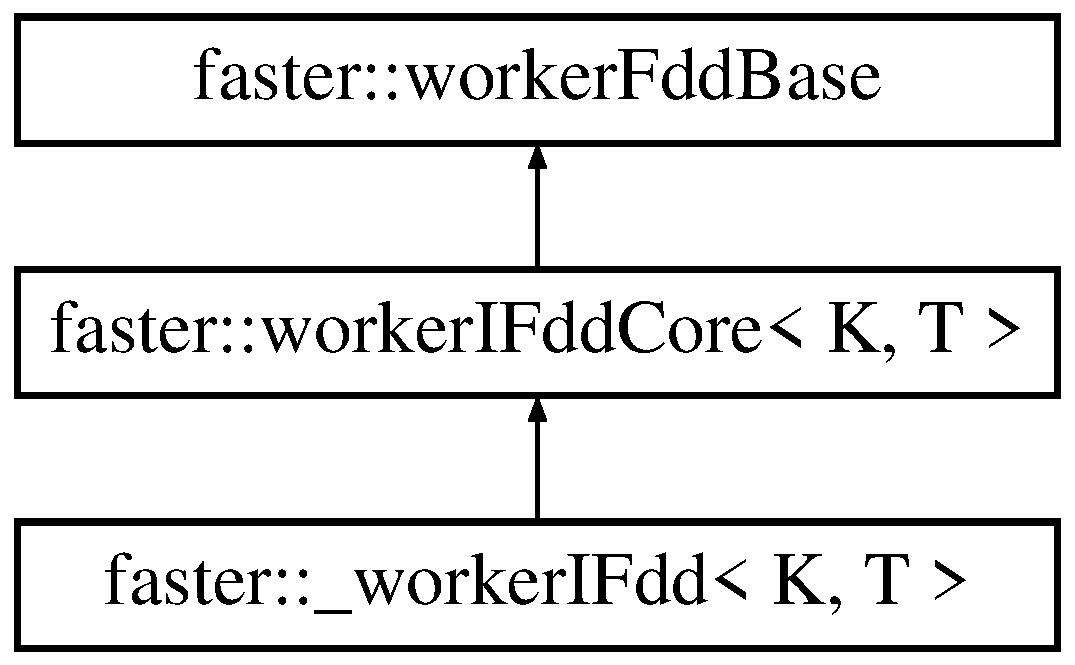
\includegraphics[height=3.000000cm]{classfaster_1_1workerIFddCore}
\end{center}
\end{figure}
\subsection*{Public Member Functions}
\begin{DoxyCompactItemize}
\item 
\hypertarget{classfaster_1_1workerIFddCore_a4870d516ed4bef37adc17746b74ec267}{}{\bfseries worker\+I\+Fdd\+Core} (unsigned int ident, fdd\+Type kt, fdd\+Type t)\label{classfaster_1_1workerIFddCore_a4870d516ed4bef37adc17746b74ec267}

\item 
\hypertarget{classfaster_1_1workerIFddCore_a5e7e471ccfa11ee3e3b5a287d6512f2f}{}{\bfseries worker\+I\+Fdd\+Core} (unsigned int ident, fdd\+Type kt, fdd\+Type t, size\+\_\+t size)\label{classfaster_1_1workerIFddCore_a5e7e471ccfa11ee3e3b5a287d6512f2f}

\item 
\hypertarget{classfaster_1_1workerIFddCore_af389368c2a1761b958c8e08336864b92}{}fdd\+Type {\bfseries get\+Type} () override\label{classfaster_1_1workerIFddCore_af389368c2a1761b958c8e08336864b92}

\item 
\hypertarget{classfaster_1_1workerIFddCore_a5db1be64cd268995e0ca456b5407510d}{}fdd\+Type {\bfseries get\+Key\+Type} () override\label{classfaster_1_1workerIFddCore_a5db1be64cd268995e0ca456b5407510d}

\item 
\hypertarget{classfaster_1_1workerIFddCore_a3effbc1108e2778555e63f655cdac4d9}{}void {\bfseries set\+Data} (void $\ast$data U\+N\+U\+S\+E\+D, size\+\_\+t size U\+N\+U\+S\+E\+D)\label{classfaster_1_1workerIFddCore_a3effbc1108e2778555e63f655cdac4d9}

\item 
\hypertarget{classfaster_1_1workerIFddCore_a1fda790a0244ace7fbf02f5d291eae1c}{}void {\bfseries set\+Data} (void $\ast$data U\+N\+U\+S\+E\+D, size\+\_\+t $\ast$ls U\+N\+U\+S\+E\+D, size\+\_\+t size U\+N\+U\+S\+E\+D)\label{classfaster_1_1workerIFddCore_a1fda790a0244ace7fbf02f5d291eae1c}

\item 
\hypertarget{classfaster_1_1workerIFddCore_ae8c350a472d39e564e1b5a9ebfdf0500}{}void {\bfseries set\+Data\+Raw} (void $\ast$data U\+N\+U\+S\+E\+D, size\+\_\+t size U\+N\+U\+S\+E\+D) override\label{classfaster_1_1workerIFddCore_ae8c350a472d39e564e1b5a9ebfdf0500}

\item 
\hypertarget{classfaster_1_1workerIFddCore_a4ef9b26a6d008c213b8fb0447aaed235}{}void {\bfseries set\+Data\+Raw} (void $\ast$data U\+N\+U\+S\+E\+D, size\+\_\+t $\ast$line\+Sizes U\+N\+U\+S\+E\+D, size\+\_\+t size U\+N\+U\+S\+E\+D) override\label{classfaster_1_1workerIFddCore_a4ef9b26a6d008c213b8fb0447aaed235}

\item 
\hypertarget{classfaster_1_1workerIFddCore_a335e2a0b88c46266ef7b92c51579fda1}{}T \& {\bfseries operator\mbox{[}$\,$\mbox{]}} (size\+\_\+t address)\label{classfaster_1_1workerIFddCore_a335e2a0b88c46266ef7b92c51579fda1}

\item 
\hypertarget{classfaster_1_1workerIFddCore_a500739e77cf51a8d4d1f33b3d0539979}{}void $\ast$ {\bfseries get\+Item} (size\+\_\+t address)\label{classfaster_1_1workerIFddCore_a500739e77cf51a8d4d1f33b3d0539979}

\item 
\hypertarget{classfaster_1_1workerIFddCore_a676cc1b789ba5f644d89cabcc55b0128}{}void $\ast$ {\bfseries get\+Data} () override\label{classfaster_1_1workerIFddCore_a676cc1b789ba5f644d89cabcc55b0128}

\item 
\hypertarget{classfaster_1_1workerIFddCore_a821f5ceafb320292d865cbdef0102baa}{}void $\ast$ {\bfseries get\+Keys} ()\label{classfaster_1_1workerIFddCore_a821f5ceafb320292d865cbdef0102baa}

\item 
\hypertarget{classfaster_1_1workerIFddCore_ad3d44ae7744b105c96f6edbc2c0246b4}{}size\+\_\+t {\bfseries get\+Size} () override\label{classfaster_1_1workerIFddCore_ad3d44ae7744b105c96f6edbc2c0246b4}

\item 
\hypertarget{classfaster_1_1workerIFddCore_a20f1bc0ed1ea0a2f63626d19d56ffb4c}{}size\+\_\+t {\bfseries item\+Size} () override\label{classfaster_1_1workerIFddCore_a20f1bc0ed1ea0a2f63626d19d56ffb4c}

\item 
\hypertarget{classfaster_1_1workerIFddCore_a6c73991bfdc0e93c08a79640e00e39b5}{}size\+\_\+t {\bfseries base\+Size} () override\label{classfaster_1_1workerIFddCore_a6c73991bfdc0e93c08a79640e00e39b5}

\item 
\hypertarget{classfaster_1_1workerIFddCore_af9fd709018ea26ff162843b4b3f2f9b1}{}void {\bfseries set\+Size} (size\+\_\+t s)\label{classfaster_1_1workerIFddCore_af9fd709018ea26ff162843b4b3f2f9b1}

\item 
\hypertarget{classfaster_1_1workerIFddCore_a1fa9b2111ed7dc167dad448d68397dcf}{}void {\bfseries delete\+Item} (void $\ast$item) override\label{classfaster_1_1workerIFddCore_a1fa9b2111ed7dc167dad448d68397dcf}

\item 
\hypertarget{classfaster_1_1workerIFddCore_a28293a19e96e13b46cbdbe58ece0df45}{}void {\bfseries shrink} ()\label{classfaster_1_1workerIFddCore_a28293a19e96e13b46cbdbe58ece0df45}

\item 
\hypertarget{classfaster_1_1workerIFddCore_a9a20510374fc95015a5c95301a3d7ee7}{}void {\bfseries preapply} (unsigned long int id, void $\ast$func, fdd\+Op\+Type op, \hyperlink{classfaster_1_1workerFddBase}{worker\+Fdd\+Base} $\ast$dest, \hyperlink{classfaster_1_1fastComm}{fast\+Comm} $\ast$comm)\label{classfaster_1_1workerIFddCore_a9a20510374fc95015a5c95301a3d7ee7}

\item 
\hypertarget{classfaster_1_1workerIFddCore_a24fcf2970ad4871bee0ccc1f0ecfca71}{}void {\bfseries group\+By\+Key} (\hyperlink{classfaster_1_1fastComm}{fast\+Comm} $\ast$comm)\label{classfaster_1_1workerIFddCore_a24fcf2970ad4871bee0ccc1f0ecfca71}

\item 
\hypertarget{classfaster_1_1workerIFddCore_a61548cbc82deeee27391b14017498bc9}{}void {\bfseries count\+By\+Key} (\hyperlink{classfaster_1_1fastComm}{fast\+Comm} $\ast$comm)\label{classfaster_1_1workerIFddCore_a61548cbc82deeee27391b14017498bc9}

\item 
\hypertarget{classfaster_1_1workerIFddCore_af9f7f09c8e1a001c676f958f2f353519}{}void {\bfseries exchange\+Data\+By\+Key} (\hyperlink{classfaster_1_1fastComm}{fast\+Comm} $\ast$comm, void $\ast$key\+Map)\label{classfaster_1_1workerIFddCore_af9f7f09c8e1a001c676f958f2f353519}

\item 
\hypertarget{classfaster_1_1workerIFddCore_a9184015edf3f3f8a74a8f4fdd2e27960}{}std\+::vector$<$ std\+::vector$<$ void $\ast$ $>$ $>$ $\ast$ {\bfseries get\+Key\+Locations} ()\label{classfaster_1_1workerIFddCore_a9184015edf3f3f8a74a8f4fdd2e27960}

\end{DoxyCompactItemize}
\subsection*{Protected Member Functions}
\begin{DoxyCompactItemize}
\item 
\hypertarget{classfaster_1_1workerIFddCore_a26fb895202e4047b8e82794719bb0eaa}{}K $\ast$ {\bfseries distribute\+Ownership} (\hyperlink{classfaster_1_1fastComm}{fast\+Comm} $\ast$comm, K $\ast$u\+Keys, size\+\_\+t c\+Size)\label{classfaster_1_1workerIFddCore_a26fb895202e4047b8e82794719bb0eaa}

\item 
\hypertarget{classfaster_1_1workerIFddCore_a160215ff486742aa4795e90e71cd8f0e}{}void {\bfseries send\+Part\+Key\+Count} (\hyperlink{classfaster_1_1fastComm}{fast\+Comm} $\ast$comm)\label{classfaster_1_1workerIFddCore_a160215ff486742aa4795e90e71cd8f0e}

\item 
\hypertarget{classfaster_1_1workerIFddCore_af5fdb0b95a8029bbe6b588fb7be45c07}{}std\+::unordered\+\_\+map$<$ K, size\+\_\+t $>$ {\bfseries recv\+Part\+Key\+Max\+Count} (\hyperlink{classfaster_1_1fastComm}{fast\+Comm} $\ast$comm, std\+::unordered\+\_\+map$<$ K, std\+::pair$<$ size\+\_\+t, std\+::deque$<$ int $>$$>$ $>$ \&key\+P\+P\+Max\+Count)\label{classfaster_1_1workerIFddCore_af5fdb0b95a8029bbe6b588fb7be45c07}

\item 
\hypertarget{classfaster_1_1workerIFddCore_a5b87c56a369a077ad1b194359f8a73bc}{}std\+::unordered\+\_\+map$<$ K, size\+\_\+t $>$ {\bfseries recv\+Part\+Key\+Count} (\hyperlink{classfaster_1_1fastComm}{fast\+Comm} $\ast$comm)\label{classfaster_1_1workerIFddCore_a5b87c56a369a077ad1b194359f8a73bc}

\item 
\hypertarget{classfaster_1_1workerIFddCore_ac15047cf51618a15489993fe3a263837}{}std\+::unordered\+\_\+map$<$ K, size\+\_\+t $>$ {\bfseries distributed\+Max\+Key\+Count} (\hyperlink{classfaster_1_1fastComm}{fast\+Comm} $\ast$comm, std\+::unordered\+\_\+map$<$ K, std\+::pair$<$ size\+\_\+t, std\+::deque$<$ int $>$$>$ $>$ \&key\+P\+P\+Max\+Count)\label{classfaster_1_1workerIFddCore_ac15047cf51618a15489993fe3a263837}

\end{DoxyCompactItemize}
\subsection*{Protected Attributes}
\begin{DoxyCompactItemize}
\item 
\hypertarget{classfaster_1_1workerIFddCore_a6bd0d4cb57e817b78276c1442bc74441}{}\hyperlink{classfaster_1_1indexedFddStorage}{indexed\+Fdd\+Storage}$<$ K, T $>$ $\ast$ {\bfseries local\+Data}\label{classfaster_1_1workerIFddCore_a6bd0d4cb57e817b78276c1442bc74441}

\item 
\hypertarget{classfaster_1_1workerIFddCore_a2b45bf1e4561a0622ad33cc8ddab6618}{}std\+::vector$<$ K $>$ {\bfseries u\+Keys}\label{classfaster_1_1workerIFddCore_a2b45bf1e4561a0622ad33cc8ddab6618}

\item 
\hypertarget{classfaster_1_1workerIFddCore_a0aae335b6c84d8927e04a486f9957ad1}{}std\+::vector$<$ std\+::vector$<$ void $\ast$ $>$ $>$ {\bfseries key\+Locations}\label{classfaster_1_1workerIFddCore_a0aae335b6c84d8927e04a486f9957ad1}

\item 
\hypertarget{classfaster_1_1workerIFddCore_a6545ef59d553976a05da0c7790264fd1}{}bool {\bfseries grouped\+By\+Key}\label{classfaster_1_1workerIFddCore_a6545ef59d553976a05da0c7790264fd1}

\end{DoxyCompactItemize}


The documentation for this class was generated from the following file\+:\begin{DoxyCompactItemize}
\item 
/home/mtcs/pesquisa/faster/faster.\+git/src/include/\+\_\+worker\+I\+Fdd.\+h\end{DoxyCompactItemize}

%--- End generated contents ---

% Index
\backmatter
\newpage
\phantomsection
\clearemptydoublepage
\addcontentsline{toc}{chapter}{Index}
\printindex

\end{document}
